%
%
%
%
%
%
%
%
\documentclass[12pt,]{article}

%% Package geometry
\usepackage[left = 2cm,right = 2cm,top = 2cm,bottom =
2cm,textheight=\paperheight]{geometry}
\usepackage{pdflscape}

% Control spacing before and after titles
\usepackage{titlesec}
% Reduce spacing before and after the Chapter title
\titleformat{\chapter}[display]
{\normalfont\huge\bfseries}{\chaptertitlename~\thechapter}{25pt}{\Huge}
\titlespacing*{\chapter}{0pt}{-50pt}{20pt}
\titlespacing*{name=\chapter,numberless}{0pt}{-50pt}{25pt}

%% Package polyglossia
\usepackage{polyglossia}
\setmainlanguage[]{french}

% Change caption name for table env
\gappto\captionsfrench{\renewcommand{\tablename}{Tableau}}
\gappto\captionsfrench{\renewcommand{\figurename}{Figure}}

%% Package fontspec
\usepackage{fontspec}
\setmainfont{STIX2Text-Regular}[
  Path           = ./fonts/,
  Extension      = .otf,
  BoldFont       = STIX2Text-Bold,
  ItalicFont     = STIX2Text-Italic,
  BoldItalicFont = STIX2Text-BoldItalic]


\usepackage{unicode-math}
\setmathfont{STIX Two Math}

\usepackage{parskip}
\setlength{\parindent}{0pt} % Remove indentation
\setlength{\parskip}{6pt plus 2pt minus 1pt}

\pagestyle{plain}
% The default `plain` pagestyle just numbers the pages,
% whereas  
% \pagestyle{empty} 
% would give you no numbering.
% After one-million man-years of macro-composition, 
% there are also fancy pagestyles with much wilder options 
% for headers and footers, of course.

% Lists formatting: 
% note sure what 'fancy enums' are; something to do with lists, 
% as the further comment suggests: 

\providecommand{\tightlist}{%
  \setlength{\itemsep}{0pt}\setlength{\parskip}{0pt}}

\usepackage{array}
\newcommand{\PreserveBackslash}[1]{\let\temp=\\#1\let\\=\temp}
\let\PBS=\PreserveBackslash

% Create new command to deal with with pandoc's super/sub script.

% Web-style links:

% markdown inclines us to use links, since our texts can be made into html. 
% Why not have clickable blue links even in 
% learned, scientific, religious, juridical, poetical and other suchlike texts? 
% Never mind that they have been proven to destroy the nervous system!

% First, what about the fact that links like http://example.com are 
% technically code and thus must not be broken across lines? 
% [breaklinks=true] to the rescue!

% Nowadays LaTeX can handle all of this with another half million macros:

\usepackage[breaklinks=true]{hyperref}
\hypersetup{colorlinks,%
citecolor=black,%
filecolor=black,%
linkcolor=black,%
urlcolor=black}
\usepackage{url}

%% Graphics
\usepackage{graphicx}
\makeatletter
\def\maxwidth{\ifdim\Gin@nat@width>\linewidth\linewidth
\else\Gin@nat@width\fi}
\makeatother
\let\Oldincludegraphics\includegraphics
\renewcommand{\includegraphics}[1]{\Oldincludegraphics[width=\maxwidth]{#1}}

\usepackage{eso-pic} % Add picture in background

% Title page
\newcommand\BackgroundPic{%
	\put(0,0){%
		\parbox[b][\paperheight]{\paperwidth}{%
			\Oldincludegraphics[height=\paperheight, width=0.25\paperwidth]{../.assets/templates/pictures/polychaeta-4.jpg}%
			\vfill
		}
	}
	% Manually positionning the picture
	\put(150,-720){
		\parbox[b][\paperheight]{\paperwidth}{%
			\Oldincludegraphics[]{../.assets/templates/pictures/logo_memoire.png}
			\vfill
		}
	}
}


\usepackage{float}
\floatplacement{figure}{H}

\usepackage{placeins}

%% linestreching
\usepackage{setspace}
\setstretch{1.241}

% Section numbering.  
% Here again is a variable you can specify on the commandline
% `markdown2pdf my.txt --number-sections --xetex --template=/wherever/this/is -o my.pdf`

\setcounter{secnumdepth}{-\maxdimen} % remove section numbering

\usepackage{caption}
\usepackage[capitalise]{cleveref}
\makeatletter
\if@cref@capitalise
\crefname{figure}{Figure}{Figure}
\crefname{table}{Tableau}{Tableau}
\else
\crefname{figure}{figure}{figure}
\crefname{table}{tableau}{tableau}
\fi
\makeatother

%% Table
\usepackage{longtable}
\usepackage{booktabs}

%% Verbatim
\usepackage{color}
\usepackage{fancyvrb}
\newcommand{\VerbBar}{|}
\newcommand{\VERB}{\Verb[commandchars=\\\{\}]}
\DefineVerbatimEnvironment{Highlighting}{Verbatim}{commandchars=\\\{\}}
% Add ',fontsize=\small' for more characters per line
\usepackage{framed}
\definecolor{shadecolor}{RGB}{248,248,248}
\newenvironment{Shaded}{\begin{snugshade}}{\end{snugshade}}
\newcommand{\KeywordTok}[1]{\textcolor[rgb]{0.13,0.29,0.53}{\textbf{#1}}}
\newcommand{\DataTypeTok}[1]{\textcolor[rgb]{0.13,0.29,0.53}{#1}}
\newcommand{\DecValTok}[1]{\textcolor[rgb]{0.00,0.00,0.81}{#1}}
\newcommand{\BaseNTok}[1]{\textcolor[rgb]{0.00,0.00,0.81}{#1}}
\newcommand{\FloatTok}[1]{\textcolor[rgb]{0.00,0.00,0.81}{#1}}
\newcommand{\ConstantTok}[1]{\textcolor[rgb]{0.00,0.00,0.00}{#1}}
\newcommand{\CharTok}[1]{\textcolor[rgb]{0.31,0.60,0.02}{#1}}
\newcommand{\SpecialCharTok}[1]{\textcolor[rgb]{0.00,0.00,0.00}{#1}}
\newcommand{\StringTok}[1]{\textcolor[rgb]{0.31,0.60,0.02}{#1}}
\newcommand{\VerbatimStringTok}[1]{\textcolor[rgb]{0.31,0.60,0.02}{#1}}
\newcommand{\SpecialStringTok}[1]{\textcolor[rgb]{0.31,0.60,0.02}{#1}}
\newcommand{\ImportTok}[1]{#1}
\newcommand{\CommentTok}[1]{\textcolor[rgb]{0.56,0.35,0.01}{\textit{#1}}}
\newcommand{\DocumentationTok}[1]{\textcolor[rgb]{0.56,0.35,0.01}{\textbf{\textit{#1}}}}
\newcommand{\AnnotationTok}[1]{\textcolor[rgb]{0.56,0.35,0.01}{\textbf{\textit{#1}}}}
\newcommand{\CommentVarTok}[1]{\textcolor[rgb]{0.56,0.35,0.01}{\textbf{\textit{#1}}}}
\newcommand{\OtherTok}[1]{\textcolor[rgb]{0.56,0.35,0.01}{#1}}
\newcommand{\FunctionTok}[1]{\textcolor[rgb]{0.00,0.00,0.00}{#1}}
\newcommand{\VariableTok}[1]{\textcolor[rgb]{0.00,0.00,0.00}{#1}}
\newcommand{\ControlFlowTok}[1]{\textcolor[rgb]{0.13,0.29,0.53}{\textbf{#1}}}
\newcommand{\OperatorTok}[1]{\textcolor[rgb]{0.81,0.36,0.00}{\textbf{#1}}}
\newcommand{\BuiltInTok}[1]{#1}
\newcommand{\ExtensionTok}[1]{#1}
\newcommand{\PreprocessorTok}[1]{\textcolor[rgb]{0.56,0.35,0.01}{\textit{#1}}}
\newcommand{\AttributeTok}[1]{\textcolor[rgb]{0.77,0.63,0.00}{#1}}
\newcommand{\RegionMarkerTok}[1]{#1}
\newcommand{\InformationTok}[1]{\textcolor[rgb]{0.56,0.35,0.01}{\textbf{\textit{#1}}}}
\newcommand{\WarningTok}[1]{\textcolor[rgb]{0.56,0.35,0.01}{\textbf{\textit{#1}}}}
\newcommand{\AlertTok}[1]{\textcolor[rgb]{0.94,0.16,0.16}{#1}}
\newcommand{\ErrorTok}[1]{\textcolor[rgb]{0.64,0.00,0.00}{\textbf{#1}}}
\newcommand{\NormalTok}[1]{#1}

\newlength{\cslhangindent}
\setlength{\cslhangindent}{1.5em}
\newenvironment{cslreferences}%
  {\setlength{\parindent}{0pt}%
  \everypar{\setlength{\hangindent}{\cslhangindent}}\ignorespaces}%
  {\par}



%% pandoc-fignos: required package


%% pandoc-fignos: change cref names
\crefname{figure}{Figure}{figs.}

%% pandoc-fignos: change Cref names
\Crefname{figure}{figure}{Figs.}

%% pandoc-eqnos: disable brackets around cleveref numbers
\creflabelformat{equation}{#2#1#3}

%% pandoc-tablenos: change cref names
\crefname{table}{Tableau}{tables}

% pandoc-tablenos: change the caption name
\renewcommand{\tablename}{Tableau}

\title{Caractériser la contribution des facteurs environnementaux et des
interactions biotiques à la variabilité des assemblages benthiques}

\author{Clément \textsc{Violet}\\}

% At last: 
% The document itself!:

% After filling in all these blanks above, or erasing them 
% where they are not needed, Pandoc has finished writing the 
% famous LaTeX *preamble* for your document.
% Now comes the all-important command \begin{document}
% which as you can see, will be paired with an \end{document} at the end.
% Pandoc knows whether you have a title, and has already
% specified what it is; if so, it demands that the title be rendered.  
% Pandoc knows whether you want a table of contents, you
% specify this on the command line.
% Then, after fiddling with alignments, there comes the real
% business: pandoc slaps its rendering of your text in the place of
% the variable `body`
% It then concludes the document it has been writing. 

\begin{document}


%\maketitle

\begin{titlepage}
	\newgeometry{top=4cm, bottom=4cm, left=5.5cm, right=1cm}
	
	\AddToShipoutPicture*{\BackgroundPic}
	\centering
	{\LARGE Université de Rennes 1 \par}
	\vspace{1cm}
	{\Large Master 2 : Modélisation en Ecologie\par}
	\vspace{1.5cm}
	{\scshape\large\bfseries Caractériser la contribution des facteurs
environnementaux et des interactions biotiques à la variabilité des
assemblages benthiques\par}
	\vspace{2cm}
	{\scshape\Large\itshape Clément Violet\par}
	\vfill
  \large \emph{Laboratoire d'Ecologie Benthique Côtière}, Centre IFREMER Brest
	\vfill
	\large Encadrants :\par
	\vspace{0.5cm}
	% \begin{tabular}{l}
	% \large \textbf{Dr Martin Marzloff}, \emph{IFREMER}, LEBCO Brest \\
	% \large Dr. Aurélien \textsc{Boyé}, \emph{IFREMER} , LEBCO, Brest \\
	% \large Dr. Olivier \textsc{Gauthier}, \emph{IUEM}, LEMAR, Brest\\
	% \large Dr. Jacques \textsc{Grall}, \emph{IUEM}, Observatoire Marin, Brest\\
	% \end{tabular}
	%
	\begin{tabular}{l}
		\large Dr Martin, \emph{IFREMER}, LEBCO, Brest\\
		\large Dr Aurélien, \emph{IFREMER}, LEBCO, Brest\\
		\large Dr Gauthier, \emph{IUEM}, LEMAR, Brest\\
		\large Dr Jacques, \emph{IUEM}, Observatoire Marin, Brest\\
		\end{tabular}

	\vfill

% Bottom of the page
	{\large\textbf{Année 2019 --- 2020}}
	
\end{titlepage}

\restoregeometry

% Roman numbering for content before toc and toc itself
\cleardoublepage 
\pagenumbering{roman}



\hypertarget{remerciements}{%
\section{Remerciements}\label{remerciements}}

Je souhaiterai remercier en premier lieu mon encadrant principal, Martin
Marzloff pour avoir eu la gentillesse de m'accepter en stage à ses
côtés. Je souhaite le remercier chaleureusement, lui et Aurélien Boyé
pour avoir patiemment répondu à mes trop nombreuses questions tout au
long de stage et pour les abondants commentaires qui ont grandement
amélioré la qualité de ce manuscrit. Je remercie également Olivier
Gauthier pour les heures de discussion passées à décortiquer les modèles
dont il est question dans ce manuscrit, ces discussions m'ont permis
d'encore approfondir mes connaissances en statistiques. Enfin Jacques
Grall pour avoir répondu à mes questions sur la biologie et les
interactions que peuvent entretenir ces animaux. Pour finir, je
souhaiterai remercier tous les experts des polychètes que j'ai
interrogés, sans qui une grande partie de ce travail n'aurait été
possible.

\hypertarget{notations-mathuxe9matiques}{%
\section{Notations mathématiques}\label{notations-mathuxe9matiques}}

\textbf{Indices}

{\small
\begin{longtable}[l]{@{}ll@{}}
\toprule
\begin{minipage}[b]{0.39\columnwidth}\raggedright
Indice \& plage de valeurs\strut
\end{minipage} & \begin{minipage}[b]{0.39\columnwidth}\raggedright
Description\strut
\end{minipage}\tabularnewline
\midrule
\endhead
\begin{minipage}[t]{0.39\columnwidth}\raggedright
\(i = 1, \dots, n\)\strut
\end{minipage} & \begin{minipage}[t]{0.39\columnwidth}\raggedright
Unité d'échantillonnage\strut
\end{minipage}\tabularnewline
\begin{minipage}[t]{0.39\columnwidth}\raggedright
\(j = 1, \dots, n_s\)\strut
\end{minipage} & \begin{minipage}[t]{0.39\columnwidth}\raggedright
Espèce\strut
\end{minipage}\tabularnewline
\begin{minipage}[t]{0.39\columnwidth}\raggedright
\(r = 1, \dots, n_r\)\strut
\end{minipage} & \begin{minipage}[t]{0.39\columnwidth}\raggedright
Effet aléatoire\strut
\end{minipage}\tabularnewline
\begin{minipage}[t]{0.39\columnwidth}\raggedright
\(l = 1, \dots, n_l\)\strut
\end{minipage} & \begin{minipage}[t]{0.39\columnwidth}\raggedright
Variable latente\strut
\end{minipage}\tabularnewline
\bottomrule
\end{longtable}}\FloatBarrier


\textbf{Vecteurs et matrices}

{\small
\begin{longtable}[l]{@{}ll@{}}
\toprule
\begin{minipage}[b]{0.34\columnwidth}\raggedright
Matrice\strut
\end{minipage} & \begin{minipage}[b]{0.60\columnwidth}\raggedright
Description\strut
\end{minipage}\tabularnewline
\midrule
\endhead
\begin{minipage}[t]{0.34\columnwidth}\raggedright
\(Y, y_{ij}\)\strut
\end{minipage} & \begin{minipage}[t]{0.60\columnwidth}\raggedright
Abondances observées\strut
\end{minipage}\tabularnewline
\begin{minipage}[t]{0.34\columnwidth}\raggedright
\(\hat{Y}, \hat{y}_{ij}\)\strut
\end{minipage} & \begin{minipage}[t]{0.60\columnwidth}\raggedright
Abondances estimées\strut
\end{minipage}\tabularnewline
\begin{minipage}[t]{0.34\columnwidth}\raggedright
\(m\)\strut
\end{minipage} & \begin{minipage}[t]{0.60\columnwidth}\raggedright
Abondances moyennes\strut
\end{minipage}\tabularnewline
\begin{minipage}[t]{0.34\columnwidth}\raggedright
\(X, x_{ij}\)\strut
\end{minipage} & \begin{minipage}[t]{0.60\columnwidth}\raggedright
Données environnementales\strut
\end{minipage}\tabularnewline
\begin{minipage}[t]{0.34\columnwidth}\raggedright
\(B, \beta_{ij}\)\strut
\end{minipage} & \begin{minipage}[t]{0.60\columnwidth}\raggedright
Coefficients associés à la niche environnementale\strut
\end{minipage}\tabularnewline
\begin{minipage}[t]{0.34\columnwidth}\raggedright
~\(Z, z_{ij}\)\strut
\end{minipage} & \begin{minipage}[t]{0.60\columnwidth}\raggedright
Variables latentes (coordonnés de sites)\strut
\end{minipage}\tabularnewline
\begin{minipage}[t]{0.34\columnwidth}\raggedright
\(\Lambda, \lambda_{ij}\)\strut
\end{minipage} & \begin{minipage}[t]{0.60\columnwidth}\raggedright
Facteurs latents (coordonnés d'espèces)\strut
\end{minipage}\tabularnewline
\begin{minipage}[t]{0.34\columnwidth}\raggedright
\(\Omega, \omega_{ij}\)\strut
\end{minipage} & \begin{minipage}[t]{0.60\columnwidth}\raggedright
Corrélations résiduelles interspécifiques\strut
\end{minipage}\tabularnewline
\bottomrule
\end{longtable}}\FloatBarrier


\textbf{Fonction et distribution statistique}

{\small
\begin{longtable}[l]{@{}ll@{}}
\toprule
\begin{minipage}[b]{0.41\columnwidth}\raggedright
Fonction / Distribution statistique\strut
\end{minipage} & \begin{minipage}[b]{0.53\columnwidth}\raggedright
Description\strut
\end{minipage}\tabularnewline
\midrule
\endhead
\begin{minipage}[t]{0.41\columnwidth}\raggedright
\(g(.)\)\strut
\end{minipage} & \begin{minipage}[t]{0.53\columnwidth}\raggedright
Fonction de lien d'un modèle linéaire généralisé\strut
\end{minipage}\tabularnewline
\begin{minipage}[t]{0.41\columnwidth}\raggedright
\(\mathcal L\)\strut
\end{minipage} & \begin{minipage}[t]{0.53\columnwidth}\raggedright
Fonction de log-vraisemblance\strut
\end{minipage}\tabularnewline
\begin{minipage}[t]{0.41\columnwidth}\raggedright
\(sgn(.)\)\strut
\end{minipage} & \begin{minipage}[t]{0.53\columnwidth}\raggedright
Fonction signe\strut
\end{minipage}\tabularnewline
\begin{minipage}[t]{0.41\columnwidth}\raggedright
\(\mathcal P(.)\)\strut
\end{minipage} & \begin{minipage}[t]{0.53\columnwidth}\raggedright
Distribution de Poisson log-normale\strut
\end{minipage}\tabularnewline
\begin{minipage}[t]{0.41\columnwidth}\raggedright
\(\mathcal N(.)\)\strut
\end{minipage} & \begin{minipage}[t]{0.53\columnwidth}\raggedright
Distribution normale\strut
\end{minipage}\tabularnewline
\bottomrule
\end{longtable}}\FloatBarrier


\textbf{Divers}

{\small
\begin{longtable}[l]{@{}ll@{}}
\toprule
\begin{minipage}[b]{0.19\columnwidth}\raggedright
Divers\strut
\end{minipage} & \begin{minipage}[b]{0.75\columnwidth}\raggedright
Description\strut
\end{minipage}\tabularnewline
\midrule
\endhead
\begin{minipage}[t]{0.19\columnwidth}\raggedright
\(y_{.j}\)\strut
\end{minipage} & \begin{minipage}[t]{0.75\columnwidth}\raggedright
~Vecteur de l'abondance de l'espèce \(j\) à travers tous les sites\strut
\end{minipage}\tabularnewline
\begin{minipage}[t]{0.19\columnwidth}\raggedright
\(r_s\)\strut
\end{minipage} & \begin{minipage}[t]{0.75\columnwidth}\raggedright
Corrélation de Spearman\strut
\end{minipage}\tabularnewline
\bottomrule
\end{longtable}}\FloatBarrier



\setcounter{table}{0}

\tableofcontents

\cleardoublepage 
\pagenumbering{arabic}


\hypertarget{introduction}{%
\section{Introduction}\label{introduction}}

L'écologie moderne s'intéresse particulièrement à la répartition des
espèces sur la surface du globe (Worm \& Tittensor
\protect\hyperlink{ref-Worm_2018}{2018}) et à la réorganisation de la
biodiversité face aux changements environnementaux en cours (Blowes
\emph{et al.} \protect\hyperlink{ref-Blowes_2019}{2019}; Magurran
\emph{et al.} \protect\hyperlink{ref-Magurran_2019}{2019}). Une
multitude d'approches théoriques et empiriques a ainsi été développée
pour comprendre les facteurs qui gouvernent la biogéographie des espèces
et prédire les patrons spatiaux et temporels de biodiversités.

La capacité de persistance d'une espèce peut être définie grâce au
concept de niche écologique tel que proposé par Hutchinson (Hutchinson
\protect\hyperlink{ref-Hutchinson_1957}{1957}). Ainsi, la niche d'une
espèce est représentée selon un hypervolume à n-dimemensions où chaque
dimension correspond à une ressource ou une condition environnementale
(Blonder \protect\hyperlink{ref-Blonder_2017}{2017}) et permet de
décrire les besoins ou la gamme de tolérance physiologique des
organismes (Sunday \emph{et al.}
\protect\hyperlink{ref-Sunday_2012}{2012}). Cette niche de Hutchinson
peut être divisée en deux niches : (1) la niche de Grinnell qui
s'intéresse plus particulièrement aux contraintes liées aux conditions
abiotiques et caractérise la niche fondamentale de l'espèce (Grinnell
\protect\hyperlink{ref-Grinnell_1917}{1917}); (2) La niche d'Elton qui
se focalise, principalement sur les interactions biotiques entre les
individus (Elton \protect\hyperlink{ref-Elton_2001}{2001}). En
considérant le rôle des interactions biotiques en complément des
contraintes environnementales, la niche d'Elton permet de décrire la
niche réalisée des espèces, qui est en réalité celle observée \emph{in
situ}.

Une des manières d'avoir accès à la niche environnementale d'une espèce
passe par l'expérimentation afin de délimiter des gammes et seuils de
tolérances physiologiques des organismes (Bates \& Morley
\protect\hyperlink{ref-Bates_2020}{2020}). Néanmoins, pour des
contraintes pratiques, ces expériences peuvent difficilement prendre en
compte les effets combinés de plusieurs facteurs abiotiques, et se
concentrent souvent sur une seule voire deux variables environnementales
(par exemple la température et la disponibilité en nourriture, ou encore
le pH pour les études marines ciblées sur les changements en cours dans
l'océan (Boyd \emph{et al.} \protect\hyperlink{ref-Boyd_2000}{2000};
Witman \emph{et al.} \protect\hyperlink{ref-Witman_2015}{2015})). Par
ailleurs, ces expérimentations en mésocosme concernent principalement
des fines échelles spatiales, temporelles et écologiques (\emph{i.e}
échelle de l'individu plutôt que de la population ou de la communauté
(Witman \emph{et al.} \protect\hyperlink{ref-Witman_2015}{2015})).
Ainsi, l'échelle de ces études expérimentales ne permet pas
d'appréhender pleinement l'ensemble des phénomènes écologiques
structurant à l'échelle de tout un écosystème (Leibold \& Chase
\protect\hyperlink{ref-Leibold_2018}{2018}). Dans un contexte de
changements globaux rapides induits par l'Homme, il est nécessaire
d'accéder à des échelles spatiales, temporelles et écologiques plus
larges (Witman \emph{et al.} \protect\hyperlink{ref-Witman_2015}{2015};
Estes \emph{et al.} \protect\hyperlink{ref-Estes_2018}{2018}), qui soit
plus en lien avec les échelles auxquelles la société bénéficie, gère et
affecte les écosystèmes (Isbell \emph{et al.}
\protect\hyperlink{ref-Isbell_2017}{2017}). La modélisation écologique
et notamment les modèles de distribution d'espèces, fournissent un outil
privilégié pour cela (Edgar \emph{et al.}
\protect\hyperlink{ref-Edgar_2016}{2016}).

\hypertarget{pruxe9dire-la-distribution-dune-espuxe8ce}{%
\subsection{Prédire la distribution d'une
espèce}\label{pruxe9dire-la-distribution-dune-espuxe8ce}}

Parmi les approches permettant d'étudier la répartition spatiale
d'espèces, les modèles de distributions d'espèces (\emph{Species
Distribution Models} ; \emph{SDM}) constituent sans conteste l'un des
outils les plus utilisés sur ces vingt dernières années (Guisan \emph{et
al.} \protect\hyperlink{ref-Guisan_2017}{2017}; Melo-Merino \emph{et
al.} \protect\hyperlink{ref-Melo_Merino_2020}{2020}). Les \emph{SDM}
reposent sur l'utilisation de variables environnementales pour expliquer
et prédire la répartition des espèces, la niche de Grinnel constituant
``la colonne vertébrale des modèles de distribution d'espèce'' (Gravel
\emph{et al.} \protect\hyperlink{ref-Gravel_2018}{2018}).

La première implémentation de \emph{SDM} est apparue à la fin des années
80 avec la méthode \emph{BIOCLIM} (Busby
\protect\hyperlink{ref-Busby_1991}{1991}). Le développement de ce type
d'approche de modélisation a notamment été favorisé par les progrès
informatiques qui les rendent faciles à mettre en oeuvre (Araújo
\emph{et al.} \protect\hyperlink{ref-Araujo_2019}{2019}; Ovaskainen \&
Abrego \protect\hyperlink{ref-Ovaskainen_2020}{2020}). Ainsi, des
\emph{SDM} ont utilisé des modèles linéaires généralisés (Hastie \&
Pregibon \protect\hyperlink{ref-Hastie_1992}{1992}), des modèles
linéaires additifs (Wood \protect\hyperlink{ref-Wood_2011}{2011}), ou
bien encore plus récemment des modèles de machine learning basée sur des
arbres (Elith \emph{et al.}
\protect\hyperlink{ref-Elith_2008}{2008})\footnote{Un tableau listant
  quelques une des méthodes de \emph{SDM} actuellement utilisées sont
  disponible dans le \cref{tbl:sdm} en annexe.}. Ces modèles permettent
uniquement de modéliser la distribution d'une seule espèce à la fois,
ils sont qualifiés de \emph{Single-species Distribution Model}.

De plus, si ces méthodes permettent de caractériser la niche potentielle
des espèces, la niche réalisée et notamment l'aspect eltonien de la
niche des espèces reste plus difficile à appréhender (Hortal \emph{et
al.} \protect\hyperlink{ref-Hortal_2015}{2015}; Dehling \& Stouffer
\protect\hyperlink{ref-Dehling_2018}{2018}). Comprendre le rôle des
interactions biotiques dans la distribution des espèces est souvent un
facteur limitant nos capacités à prédire les patrons spatiaux de
biodiversité.

\hypertarget{pruxe9dire-la-distribution-et-les-dynamiques-des-assemblages-despuxe8ces}{%
\subsection{Prédire la distribution et les dynamiques des assemblages
d'espèces}\label{pruxe9dire-la-distribution-et-les-dynamiques-des-assemblages-despuxe8ces}}

Si la question de recherche s'intéresse à la communauté dans son
entièreté, il existe deux stratégies différentes pour modéliser la
distribution de multiples espèces. Il est possible de prédire la
distribution des espèces indépendamment et de les assembler en
communauté ensuite (\emph{Stack Species Distribution Model} ou
\emph{SSDM}), ou bien de prédire la distribution des espèces
conjointement (\emph{Joint Species Distribution Model}) (Ferrier \&
Guisan \protect\hyperlink{ref-Ferrier_2006}{2006}).

A l'inverse de l'approche climatologique largement appliquée dans le cas
des \emph{SDM} ou des \emph{SSDM} qui vise à caractériser la répartition
biogéographique des espèces, en ne considérant que très rarement les
dynamiques temporelles de manières explicites, les \emph{JSDM} ont pour
objectif de caractériser et de prédire la variabilité spatio-temporelle
des communautés. Ils permettent par ailleurs d'intégrer des informations
spécifiques additionnelles afin de tirer profit des similitudes entre
espèces à l'échelle de la communauté, notamment via les traits
fonctionnels ou encore la phylogénie (\cref{tbl:jsdm}).

De plus, les \emph{SSDM}, en combinant des modèles faits indépendamment
pour chaque espèce, ne tiennent pas compte du filtre biotique que les
espèces exercent les unes sur les autres et négligent donc l'aspect
eltonien de leur niche (Zurell \emph{et al.}
\protect\hyperlink{ref-Zurell_2019}{2019}). Au contraire, les
\emph{JSDM} ont été développés en prenant en compte les patrons de
co-occurrence à l'échelle d'une communauté afin de modéliser
conjointement la distribution de chaque espèce au sein de toute la
communauté en tenant compte des filtres abiotiques (Warton \emph{et al.}
\protect\hyperlink{ref-warton2015}{2015}). Cette structure de
co-occurrence fournit alors des informations potentielles sur les
interactions entre espèces (Ovaskainen \emph{et al.}
\protect\hyperlink{ref-Ovaskainen_2017b}{2017}\protect\hyperlink{ref-Ovaskainen_2017b}{a}).

{\small
\begin{longtable}[]{@{}llllll@{}}
\caption{Quelques uns des modèles de \emph{JSDM} et leurs
fonctionnalités (adapté de Ovaskainen \& Abrego
(\protect\hyperlink{ref-Ovaskainen_2020}{2020})). Les colonnes ``traits
fonctionnels'' et ``phylogénie'' indiquent si les modèles prennent en
compte ces données de façon explicite. \label{tbl:jsdm}}\tabularnewline
\toprule
\begin{minipage}[b]{0.35\columnwidth}\raggedright
\emph{Joint species distribution model}\strut
\end{minipage} & \begin{minipage}[b]{0.10\columnwidth}\raggedright
Effets spatiaux\strut
\end{minipage} & \begin{minipage}[b]{0.10\columnwidth}\raggedright
Effets temporels\strut
\end{minipage} & \begin{minipage}[b]{0.12\columnwidth}\raggedright
Traits fonctionnels\strut
\end{minipage} & \begin{minipage}[b]{0.07\columnwidth}\raggedright
Phylogénie\strut
\end{minipage} & \begin{minipage}[b]{0.10\columnwidth}\raggedright
Référence\strut
\end{minipage}\tabularnewline
\midrule
\endfirsthead
\toprule
\begin{minipage}[b]{0.35\columnwidth}\raggedright
\emph{Joint species distribution model}\strut
\end{minipage} & \begin{minipage}[b]{0.10\columnwidth}\raggedright
Effets spatiaux\strut
\end{minipage} & \begin{minipage}[b]{0.10\columnwidth}\raggedright
Effets temporels\strut
\end{minipage} & \begin{minipage}[b]{0.12\columnwidth}\raggedright
Traits fonctionnels\strut
\end{minipage} & \begin{minipage}[b]{0.07\columnwidth}\raggedright
Phylogénie\strut
\end{minipage} & \begin{minipage}[b]{0.10\columnwidth}\raggedright
Référence\strut
\end{minipage}\tabularnewline
\midrule
\endhead
\begin{minipage}[t]{0.35\columnwidth}\raggedright
\emph{Bayesian ordination and regression analysis} (\emph{BORAL})\strut
\end{minipage} & \begin{minipage}[t]{0.10\columnwidth}\raggedright
Implicite\strut
\end{minipage} & \begin{minipage}[t]{0.10\columnwidth}\raggedright
Implicite\strut
\end{minipage} & \begin{minipage}[t]{0.12\columnwidth}\raggedright
Oui\strut
\end{minipage} & \begin{minipage}[t]{0.07\columnwidth}\raggedright
Non\strut
\end{minipage} & \begin{minipage}[t]{0.10\columnwidth}\raggedright
Hui (\protect\hyperlink{ref-Hui_2016}{2016})\strut
\end{minipage}\tabularnewline
\begin{minipage}[t]{0.35\columnwidth}\raggedright
\emph{Hierachical modelling of Species Communities} (\emph{HMSC})\strut
\end{minipage} & \begin{minipage}[t]{0.10\columnwidth}\raggedright
Explicite\strut
\end{minipage} & \begin{minipage}[t]{0.10\columnwidth}\raggedright
Explicite\strut
\end{minipage} & \begin{minipage}[t]{0.12\columnwidth}\raggedright
Oui\strut
\end{minipage} & \begin{minipage}[t]{0.07\columnwidth}\raggedright
Oui\strut
\end{minipage} & \begin{minipage}[t]{0.10\columnwidth}\raggedright
Ovaskainen \emph{et al.}
(\protect\hyperlink{ref-Ovaskainen_2017a}{2017}\protect\hyperlink{ref-Ovaskainen_2017a}{b})\strut
\end{minipage}\tabularnewline
\begin{minipage}[t]{0.35\columnwidth}\raggedright
\emph{Generalized linear latent variable models} (\emph{GLLVM})\strut
\end{minipage} & \begin{minipage}[t]{0.10\columnwidth}\raggedright
Implicite\strut
\end{minipage} & \begin{minipage}[t]{0.10\columnwidth}\raggedright
Implicite\strut
\end{minipage} & \begin{minipage}[t]{0.12\columnwidth}\raggedright
Oui\strut
\end{minipage} & \begin{minipage}[t]{0.07\columnwidth}\raggedright
Non\strut
\end{minipage} & \begin{minipage}[t]{0.10\columnwidth}\raggedright
Niku \emph{et al.}
(\protect\hyperlink{ref-Niku_2019}{2019}\protect\hyperlink{ref-Niku_2019}{b})\strut
\end{minipage}\tabularnewline
\begin{minipage}[t]{0.35\columnwidth}\raggedright
\emph{Poisson lognormal model} (\emph{PLN})\strut
\end{minipage} & \begin{minipage}[t]{0.10\columnwidth}\raggedright
Implicite\strut
\end{minipage} & \begin{minipage}[t]{0.10\columnwidth}\raggedright
Implicite\strut
\end{minipage} & \begin{minipage}[t]{0.12\columnwidth}\raggedright
Non\strut
\end{minipage} & \begin{minipage}[t]{0.07\columnwidth}\raggedright
Non\strut
\end{minipage} & \begin{minipage}[t]{0.10\columnwidth}\raggedright
Chiquet \emph{et al.} (\protect\hyperlink{ref-Chiquet_2019}{2019})\strut
\end{minipage}\tabularnewline
\bottomrule
\end{longtable}}\FloatBarrier


\hypertarget{comprendre-le-ruxf4le-des-interactions-biotiques}{%
\subsection{Comprendre le rôle des interactions
biotiques}\label{comprendre-le-ruxf4le-des-interactions-biotiques}}

Bien que le rôle des interactions biotiques dans la structure des
communautés et la coexistence des espèces est depuis longtemps reconnu
(Hardin \protect\hyperlink{ref-Hardin_1960}{1960}; Paine
\protect\hyperlink{ref-Paine_1966}{1966}), leur influence à larges
échelles a pendant longtemps été négligée. Ainsi, l'explication des
patrons biogéographique de diversité s'est concentrée sur le rôle des
filtres abiotiques (Tittensor \emph{et al.}
\protect\hyperlink{ref-Tittensor_2010}{2010}; Soininen
\protect\hyperlink{ref-Soininen_2014}{2014}).La contribution des
interactions biotiques aux patrons de biodiversité à larges échelles est
à ce jour mal appréhendée (Wisz \emph{et al.}
\protect\hyperlink{ref-Wisz_2012}{2012}). Leur importance est néanmoins
variable dans le temps, dans l'espace et selon les systèmes biologiques
(Leibold \& Chase \protect\hyperlink{ref-Leibold_2018}{2018}). Par
exemple, la compétition pour l'espace et la prédation sont localement
des facteurs extrêmement structurants pour les communautés benthiques
des estrans rocheux. La compétition entre les balanes et les moules est
un exemple classique en écologie intertidale de compétition pour le
substrat (Hawkins \emph{et al.}
\protect\hyperlink{ref-Hawkins_2019}{2019}). De même, le rôle de la
prédation des étoiles de mer sur les balanes et sur les moules est à
l'origine du concept d'espèce «~clé de voute~» (Paine
\protect\hyperlink{ref-Paine_1966}{1966}). A contrario, les plages de
sable sont moins structurées par les interactions que les estrans
rocheux et sont généralement plus structurées par les forces
hydrodynamiques et autres facteurs abiotiques (Defeo \& McLachlan
\protect\hyperlink{ref-Defeo_2005}{2005}; Woodin \emph{et al.}
\protect\hyperlink{ref-Woodin_2019}{2019}). Clarifier le rôle relatif
des interactions biotiques par rapport aux filtres environnementaux dans
différents systèmes et à différentes échelles paraît alors primordial.

Observer et quantifier les interactions dans les écosystèmes marins est
une tâche difficile. Pour les écosystèmes pélagiques, il est possible
d'utiliser différentes techniques comme l'observation directe, l'étude
des contenus stomacaux ou bien l'analyse isotopique d'acides gras (Majdi
\emph{et al.} \protect\hyperlink{ref-Majdi_2018}{2018}). Lorsque ces
méthodes sont difficiles à mettre en place, comme c'est le cas pour les
écosystèmes benthiques aux larges échelles qui nous intéressent ici,
Majdi \emph{et al.} (\protect\hyperlink{ref-Majdi_2018}{2018}) proposent
d'utiliser des méthodes d'inférences statistiques. Ainsi, les
\emph{JSDM} peuvent être des outils intéressants pour mieux comprendre
les interactions biotiques des écosystèmes intertidaux benthiques.

\hypertarget{objectifs-scientifiques}{%
\subsection{Objectifs scientifiques}\label{objectifs-scientifiques}}

Différentes implémentations de ces modèles conjoints de distribution
d'espèces (\cref{tbl:jsdm}) ont vu le jour ces dernières années sous
l'influence forte de théorie issue de l'écologie végétale concernant le
rôle des interactions dans la structuration des communautés de plantes à
larges échelles spatiales et temporelles (Warton \emph{et al.}
\protect\hyperlink{ref-warton2015}{2015}). De récents travaux se sont
intéressés à comparer certaines de ces méthodes. Norberg \emph{et al.}
(\protect\hyperlink{ref-Norberg_2020}{2019}) ont comparé trente-trois
modèles de distributions d'espèces sur des jeux de données de
présence/absence de communautés végétales. Momal \emph{et al.}
(\protect\hyperlink{ref-Momal_2020}{2020}) quant à eux ont comparé la
capacité de reconstruction de réseaux d'interaction à partir de
résultats de modèles \emph{JSDM} entrainés sur des données d'abondance
d'une communauté de poissons et sur des données de métabarcoding issu
d'une communauté fongique. Niku \emph{et al.}
(\protect\hyperlink{ref-Niku_2019}{2019}\protect\hyperlink{ref-Niku_2019}{b})
quant à eux présentaient le \emph{JSDM} qu'ils ont développé, et son
application à une commutée de fourmis.

Le but global de ce travail est d'explorer le potentiel de différentes
méthodes de \emph{JSDM} pour expliquer et prédire la diversité
benthique. Ainsi, ce travail vise à exploiter 8 ans de données de suivi
côtier (programme \emph{REBENT};
\href{http://www.sb-roscoff.fr/fr/observation/programmes/rebent-suivi-stationnel-des-sables-sublittoraux}{www.rebent.fr})
afin de caractériser l'influence des processus biotiques et abiotiques
dans la variabilité des communautés de macrofaune benthique. En effet,
la structure des \emph{JSDM} nous permet de quantifier l'influence des
facteurs abiotiques sur les patrons spatiotemporels de biodiversité
benthique et d'appréhender les interactions biotiques à l'échelle de la
communauté. Pour ce faire, nous allons nous concentrer sur trois
implémentations différentes des JSDM : l'un des meilleurs cadres de
modélisation décrits par Norberg \emph{et al.}
(\protect\hyperlink{ref-Norberg_2020}{2019}) (\emph{HMSC} pour
\emph{Hierarchical Modelling of Species Community}), celui utilisé par
Momal \emph{et al.} (\protect\hyperlink{ref-Momal_2020}{2020})
(\emph{PLN} pour \emph{Poisson Lognormal Model}) ) et celui développé
par Niku \emph{et al.}
(\protect\hyperlink{ref-Niku_2019}{2019}\protect\hyperlink{ref-Niku_2019}{b})
(\emph{GLLVM} pour \emph{Generalised Linear Latent Variable Model}).
L'application de ces trois méthodes sur les mêmes données d'abondance
faunistiques permettra par la même occasion de comparer la performance
de ces modèles, puisqu'à notre connaissance aucune étude n'a comparé ces
trois méthodes lorsqu'elles sont appliquées aux écosystèmes benthiques.
L'innovation de cette étude est donc double~: effectuer la première
comparaison simultanée de ces trois modèles, et effectuer une des
premières approches de \emph{JSDM} sur de la faune benthique inféodée
aux habitats meubles.

\hypertarget{matuxe9riel-et-muxe9thode}{%
\section{Matériel et méthode}\label{matuxe9riel-et-muxe9thode}}

\hypertarget{cas-duxe9tude}{%
\subsection{Cas d'étude}\label{cas-duxe9tude}}

\hypertarget{jeu-de-donnuxe9es}{%
\subsubsection{Jeu de données}\label{jeu-de-donnuxe9es}}

Le jeu de donnée utilisé dans ce travail est issu du \emph{REseau de
surveillance BENthique}. Ce réseau de surveillance a été créé en 1999 à
la suite du naufrage du pétrolier Erika. Le but de ce réseau est
d'acquérir des connaissances sur les habitats benthiques côtiers et de
détecter des changements de la diversité biologique de ces habitats
(Derrien-Courtel \emph{et al.}
\protect\hyperlink{ref-Rebent2016}{2017}). Le protocole de suivis se
concentre sur la macrofaune (\textgreater{} 1mm) et la méthodologie
détaillée est présentée dans Boyé \emph{et al.}
(\protect\hyperlink{ref-Boye_2019a}{2019}). Seulement deux de ces
habitats ont été retenus pour comparer les trois méthodes de
modélisations : les herbiers de zostères et les sédiments meubles nus.

Les zostères sont des phanérogames marines qui lorsque leur densité est
forte, créent des ``herbiers''. En Bretagne, il existe deux espèces de
zostères : la zostère marine (\emph{Zostera marina}) et la zostère naine
(\emph{Zostera noltii}). Ces herbiers forment des habitats pour de
nombreuses espèces. Ils ont un rôle fonctionnel important pour beaucoup
d'espèces en tant que zone de nurserie, de reproduction et de
nourrissage (McDevitt-Irwin \emph{et al.}
\protect\hyperlink{ref-McDevitt_Irwin_2016}{2016}; Lefcheck \emph{et
al.} \protect\hyperlink{ref-Lefcheck_2019}{2019}). Cet habitat est connu
pour sa plus grande richesse spécifique par rapport à d'autres habitats
comme les sédiments meublent nus~(Hily \& Bouteille
\protect\hyperlink{ref-Hily_1999}{1999}; Sunday \emph{et al.}
\protect\hyperlink{ref-Sunday_2016}{2016}; Boyé \emph{et al.}
\protect\hyperlink{ref-Boye_2017}{2017}). Le suivi du \emph{REBENT} se
concentre sur les herbiers de \emph{Z. marina}, car cette espèce fait
déjà partie du livre rouge des espèces menacées (Waycott \emph{et al.}
\protect\hyperlink{ref-Waycott_2009}{2009}; Derrien-Courtel \emph{et
al.} \protect\hyperlink{ref-Rebent2016}{2017}). Toutefois, les mesures
de protections mises en place vis-vis de cet habitat semblent porter
leurs fruits en Europe (Santos \emph{et al.}
\protect\hyperlink{ref-de_los_Santos_2019}{2019}).

Les plages de sable abritent des communautés dominées par les crustacés
les mollusques et les polychètes (Defeo \& McLachlan
\protect\hyperlink{ref-Defeo_2005}{2005}). Cet habitat est contraint
principalement par trois facteurs abiotiques : les marées, la houle et
le sédiment. L'interaction entre ces trois facteurs crée un grand
éventail de plages différentes : de la plage où la mer ne se retire que
très peu à marée basse aux plages dont de vastes étendues de sable sont
découvertes lors des grandes marées (Defeo \& McLachlan
\protect\hyperlink{ref-Defeo_2005}{2005}). La richesse spécifique sur
ces plages est fortement influée par la hauteur des marées et dans une
moindre mesure par la température de l'eau et la taille des sédiments
(Defeo \& McLachlan \protect\hyperlink{ref-Defeo_2013}{2013}; Defeo
\emph{et al.} \protect\hyperlink{ref-Defeo_2017}{2017}). Ces plages de
sable fin ont aussi un rôle écologique important de nurserie pour de
nombreuses espèces de poissons plats (Quillien \emph{et al.}
\protect\hyperlink{ref-Quillien_2017}{2017}). Toutefois, les plages de
sable sont des biocénoses menacées. Ce sont des habitats à la fois
menacés par les changements globaux (hausse du niveau des mers,
érosion\ldots) et par les activités anthropiques telles que l'urbanisme
ou bien les activités récréatives (Defeo \emph{et al.}
\protect\hyperlink{ref-Defeo_2009}{2009}).

\hypertarget{communautuxe9-faunistique}{%
\subsubsection{Communauté faunistique}\label{communautuxe9-faunistique}}

Ce travail se concentre sur les assemblages de polychètes,du phylum des
annélides (Lecointre \& Le Guyader
\protect\hyperlink{ref-Lecointre_2001}{2001}). Cette classe a été
choisie, car composée de taxons aux modes de vie très divers, dont
l'écologie a déjà fait l'objet d'un travail approfondi (Boyé \emph{et
al.} \protect\hyperlink{ref-Boye_2019a}{2019}). Il est classique de
catégoriser les polychètes en plusieurs groupes en fonction de leurs
modes de vie : certains sont nageurs, ou tubicoles, ou bien encore
benthiques fouisseurs. Leurs régimes alimentaires sont aussi très
variés, il existe des polychètes prédateurs, mais également des
brouteurs, des suspensivores ou psamivores (Jumars \emph{et al.}
\protect\hyperlink{ref-Jumars_2015}{2015}). Toutefois, la taxonomie et
l'écologie de ces animaux restent assez mal connues par la communauté
scientifique (Troudet \emph{et al.}
\protect\hyperlink{ref-Troudet_2017}{2017}). En particulier, les
interactions écologiques (compétition pour l'espace ou la nourriture,
voire prédation) au sein de ces communautés de polychètes laissent
largement méconnues.

\hypertarget{emprise-spatiale-et-temporelle-de-luxe9tude}{%
\subsection{Emprise spatiale et temporelle de
l'étude}\label{emprise-spatiale-et-temporelle-de-luxe9tude}}

Vingt-trois sites le long de la façade bretonne ont été retenus,
représentant 215 échantillons collectés sur une période s'étalant entre
2006 et 2014. . Les données considérées contiennent 96 taxa différents
de polychètes (et le jeu de données d'apprentissage ne contient
toutefois que 92 taxa en raison de l'exclusion des 3 sites de
validation). Il est important de noter que certains sites présentent
deux habitats (\emph{i.e.} herbiers, sédiments nus) associés aux mêmes
conditions environnementales (étant donné la faible résolution spatiale
des variables environnementales). Afin de tester la performance des
modèles, vingt sites ont été retenus pour l'entraînement des différents
modèles et trois pour la validation croisée (fig.~\ref{fig:sitemap}).

\begin{figure}
\hypertarget{fig:sitemap}{%
\centering
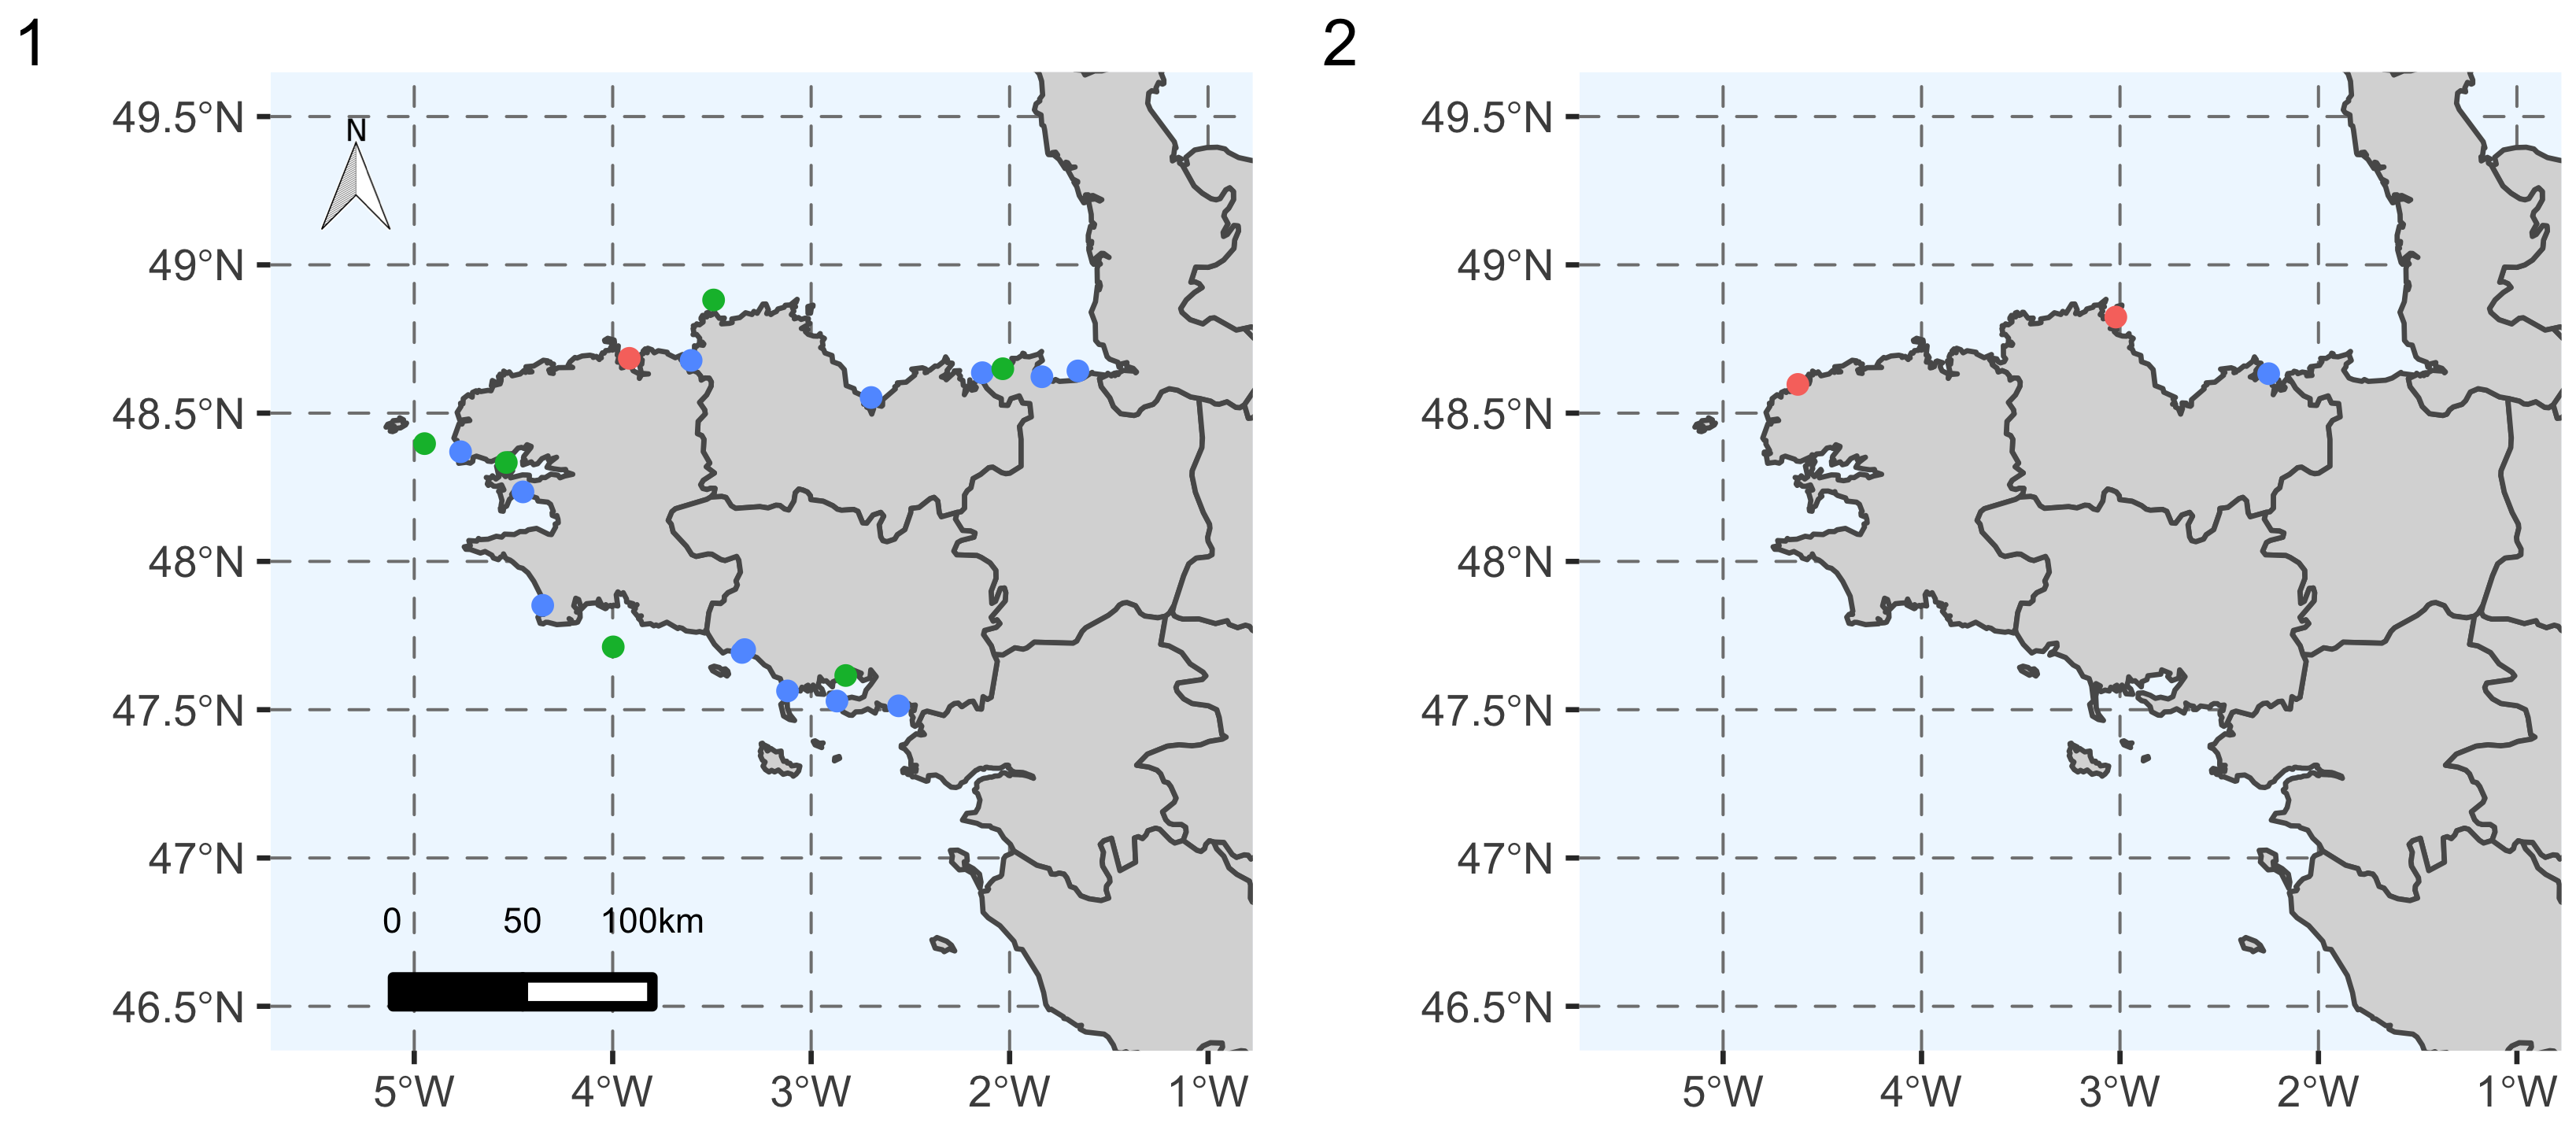
\includegraphics{figures/site_map.png}
\caption{Carte des sites échantillonnés. Les points bleus et verts
représentent respectivement les sites à sédiments meubles et les
herbiers. Les points rouges représentent les sites ayant les deux
habitats. 1. Sites utilisés pour entrainer les modèles. 2. Sites
utilisés pour valider les modèles}\label{fig:sitemap}
}
\end{figure}

\hypertarget{donnuxe9es-environnementales}{%
\subsubsection{Données
environnementales}\label{donnuxe9es-environnementales}}

Six variables environnementales, collectées lors de travaux précédents
sur ces communautés (Boyé \emph{et al.}
\protect\hyperlink{ref-Boye_2019a}{2019}) ont été sélectionnées pour
expliquer la variabilité de ces communautés (tableau : \ref{tbl:env}).
La salinité, la température et la vitesse des courants proviennent de la
base de données publique \emph{PREVIMER} basée sur les résultats des
modèles de \emph{MARS3D}. Le fetch a été calculé à partir des polygones
terrestres disponibles dans \emph{OpenStreetMap}. Les variables
granulométriques ont été échantillonnées \emph{in situ} (protocole
détaillé dans Boyé \emph{et al.}
(\protect\hyperlink{ref-Boye_2017}{2017})). Il est important de noter
que, dans le but d'utiliser des polynômes pour modéliser des relations
non linéaires, l'ensemble des variables explicatives ont été centrées et
transformées via la fonction poly. Cependant, étant donné le grand
nombre d'échantillons, nous avons été contraints d'utiliser des
polynômes de degré un, ce qui revient à modéliser une simple relation
linéaire, afin de réduire le temps de calcul.

{\small
\begin{longtable}[]{@{}lll@{}}
\caption{Variables environnementales utilisées dans l'ensemble des
modèles. \label{tbl:env}}\tabularnewline
\toprule
Abréviation & Définition & Unité\tabularnewline
\midrule
\endfirsthead
\toprule
Abréviation & Définition & Unité\tabularnewline
\midrule
\endhead
Fetch & Fetch moyen & Km\tabularnewline
MO & Concentration en Matière organique & \%\tabularnewline
SAL\_sd & Ecart-type de la salinité de l'eau & PSS-78\tabularnewline
TEMP\_sd & Ecart-type de la température de l'eau & °C~\tabularnewline
CURR\_mean & Force moyenne des courants &
~m.s\textsuperscript{-1}\tabularnewline
Mud & Concentration de boue dans les sédiments & \%\tabularnewline
Trask\_So & ~Indice de Trask - Homogénéité du sédiment &
Aucune\tabularnewline
\bottomrule
\end{longtable}}\FloatBarrier


\hypertarget{moduxe8le-de-distribution-despuxe8ces-conjointes-jsdm}{%
\subsection{\texorpdfstring{Modèle de distribution d'espèces conjointes
(\emph{JSDM})}{Modèle de distribution d'espèces conjointes (JSDM)}}\label{moduxe8le-de-distribution-despuxe8ces-conjointes-jsdm}}

Bien que chaque implémentation des \emph{JSDM} soit différente et
permettent de prendre en compte différents types de données
(\cref{tbl:jsdm}), ces modèles sont tous des extensions multivariées à
variables latentes des modèles linéaires généralisés classiques (Hui
\protect\hyperlink{ref-Hui_2016}{2016} ; Ovaskainen \emph{et al.}
\protect\hyperlink{ref-Ovaskainen_2017a}{2017}\protect\hyperlink{ref-Ovaskainen_2017a}{b};
Chiquet \emph{et al.} \protect\hyperlink{ref-Chiquet_2019}{2019}; Niku
\emph{et al.}
\protect\hyperlink{ref-Niku_2019}{2019}\protect\hyperlink{ref-Niku_2019}{b}).
Un modèle à variables latentes (\emph{LVM}) avec une variable
explicative peut être écrit comme suit\footnote{L'ensemble des notations
  mathématiques sont présentées dans le glossaire.} :

\begin{equation} y_{ij} = g\left(x_{i} \times \beta_j + Z_{i.} \times \lambda_{j.}\right) \label{eq:lvm}\end{equation}

Avec \(y_{ij}\) représentant l'abondance prédite de l'espèce \(j\) au
site \(i\). \(g(.)\) une fonction de lien ; \(x_i\) le vecteur de la
variable environnementale au site \(i\), \(\beta_j\) le coefficient de
l'effet environnemental associé pour l'espèce \(j\). Enfin, avec
\(Z_i.\) est la matrice de variable latente associée aux sites et et qui
joue le rôle des prédicteurs manquants et \(\lambda_j\) la matrice de
poids associés à l'espèce \(j\) qui donnent une estimation des
corrélations résiduelles entre espèces \(\Omega\), avec (Warton \emph{et
al.} \protect\hyperlink{ref-warton2015}{2015}) :

\begin{equation}\left(Z_i \times \lambda_j\right) \sim \mathcal{N}\left(0, \Omega\right)\label{eq:lvmconst}\end{equation}

Outre la prise en compte via les variables latentes d'éventuelles
variables explicatives manquantes et des corrélations résiduelles entre
espèces. L'avantage majeur des \emph{LVM} est que l'estimation de
matrice de corrélation entre espèces est plus simple que par rapport à
un modèle linéaire à effets mixtes généralisés. La matrice de coordonnés
des espèces (\(\lambda\)) dans le cas d'un \emph{LVM} a au plus autant
de colonnes que de variables latentes (\cref{eq:lvmconst}). Dans le cas
d'un modèle linéaire à effets mixte généralisé celle-ci à autant de
colonnes que d'espèces (Warton \emph{et al.}
\protect\hyperlink{ref-warton2015}{2015}). Ainsi, le nombre de variables
latentes utilisées par le modèle est donc un paramètre crucial,
puisqu'il permet de faire un compromis entre précisions de la matrice de
corrélation résiduelle et la réduction du temps de calcul et des degrés
de liberté utilisés (Warton \emph{et al.}
\protect\hyperlink{ref-warton2015}{2015}). Trois cadres de modélisations
ont été sélectionnés : \emph{HMSC}, \emph{GLLVM} et \emph{PLN} et
exploré cinq variantes de modèles ces modèles. L'ensemble des
caractéristiques de ces variantes de modèles sont présentées dans le
\cref{tbl:summarymod} .

\hypertarget{hierachical-modelling-of-species-communities}{%
\subsubsection{\texorpdfstring{\emph{Hierachical modelling of Species
Communities}}{Hierachical modelling of Species Communities}}\label{hierachical-modelling-of-species-communities}}

\emph{HMSC} est un modèle mixte linéaire généralisé, hiérarchique et
multivarié, ajusté par inférence bayésienne (Ovaskainen \& Abrego
\protect\hyperlink{ref-Ovaskainen_2020}{2020}). La particularité de ce
modèle est qu'il est hiérarchique, ainsi chaque effet aléatoire donne
lieu à sa propre matrice de corrélation résiduelle (Ovaskainen \emph{et
al.}
\protect\hyperlink{ref-Ovaskainen_2017a}{2017}\protect\hyperlink{ref-Ovaskainen_2017a}{b})
et qu'il peut s'implémenter avec une vaste gamme de distribution
(Tikhonov \emph{et al.}
\protect\hyperlink{ref-Tikhonov_2019b}{2019}\protect\hyperlink{ref-Tikhonov_2019b}{a}).
L'\cref{eq:hmsc} présente la formulation mathématique d'un modèle
n'utilisant que des variables environnementales et un nombre \(n_r\)
d'effets aléatoires (il serait aussi possible d'ajouter des données de
traits et de phylogénie pour mieux caractériser les niches abiotiques
des taxa similaires).

\begin{equation} y_{ij} = g\left(x_i \times \beta_j + \sum_{r = 1}^{n_r} Z_{ir} \times \lambda_{rj}\right) \label{eq:hmsc}\end{equation}

Etant un modèle bayésien, la distribution a posteriori est
échantillonnée grâce à la méthode MCMC (Ovaskainen \emph{et al.}
\protect\hyperlink{ref-Ovaskainen_2017b}{2017}\protect\hyperlink{ref-Ovaskainen_2017b}{a}).
L'utilisation de l'inférence bayésienne permet à l'utilisateur de ne pas
spécifier le nombre de variables latentes à utiliser pour chaque effet
aléatoire. Le modèle ajuste le nombre de variables latentes pour que
celles non significatives soient tronquées (Ovaskainen \& Abrego
\protect\hyperlink{ref-Ovaskainen_2020}{2020}).

Trois modèles \emph{HMSC} ont été créés : un premier sans l'inclusion
d'effets aléatoires (\emph{HMSC\_reg}) qui ne prend donc pas en compte
les corrélations résiduelles entre espèces et l'aspect eltonien de leur
niche ; un second avec un seul effet aléatoire lié à l'échantillon
(\emph{HMSC\_samp}) et un dernier avec trois facteurs aléatoires liés
respectivement à l'année, au site et à l'habitat. Ce dernier modèle
permet ainsi de partitionner les associations résiduelles entre
association temporelle, spatiale ou liée à l'habitat (sédiment nu ou
herbiers). Les calculs ont été réalisés avec le package \emph{Hmsc}
(Tikhonov \emph{et al.}
\protect\hyperlink{ref-Tikhonov_2019b}{2019}\protect\hyperlink{ref-Tikhonov_2019b}{a},
\protect\hyperlink{ref-Hmsc_2019}{b}). Chaque modèle dispose de quatre
chaînes de Markov et chaque chaîne effectue 1,5 million d'itérations
avant de se stopper. L'étape de \emph{burn-in} supprime les 500 000
premières itérations de chaque chaîne. Les chaînes sont échantillonnées
toutes les mille itérations. Les priors par défaut ont été utilisés.
Avant de regarder les résultats des différents modèles du framework
\emph{HMSC}, la validité de ces modèles a été inspectée. La bonne
convergence des chaînes a été vérifiée à l'aide de l'outil de diagnostic
de Gelman-Rubin (Gelman \& Rubin
\protect\hyperlink{ref-Gelman_1992}{1992}). Enfin, le nombre
d'échantillons indépendants pour chaque paramètre a été jugé
satisfaisant (supérieur à 1000 échantillons indépendants pour l'ensemble
des paramètres).

\hypertarget{moduxe8le-de-poisson-lognormal}{%
\subsubsection{Modèle de Poisson
Lognormal}\label{moduxe8le-de-poisson-lognormal}}

Le modèle de Poisson lognormal est linéaire mixte et multivarié. Son
implémentation ne permet de modéliser qu'une seule sorte de distribution
: la distribution (conditionnelle) de Poisson lognormale \cref{eq:pln}.
Un modèle simple avec uniquement des variables environnementales peut
être écrit de cette façon :

\begin{equation}y_{ij}|Z_{ij} \sim \mathcal P\left(exp\left\{x_i \times \beta_j + Z_{ij}\right\}\right)\label{eq:pln}\end{equation}

Le vecteur latent \(Z_i\) prend en compte les variations d'abondance non
expliquées par les variables environnementales incluses dans le modèle
(Momal \emph{et al.} \protect\hyperlink{ref-Momal_2020}{2020}). Cette
variable latente agit comme un effet aléatoire lié à l'échantillon
(Momal \emph{et al.} \protect\hyperlink{ref-Momal_2020}{2020}). Dans ce
cadre de modélisation, il y a autant de variables latentes différentes
qu'il y a d'espèces \(n_s\) et chaque variable latente suit une loi
normale de moyenne 0 et de variance \(\Omega^{-1}\), où \(\Omega\) est
la matrice de corrélations résiduelles entre espèces :

\begin{equation}Z_i \sim N\left(0_{n_s}, \Omega^{-1}\right) \label{eq:constpln}\end{equation}

Le modèle a été créé avec le package R \emph{PLNmodels} (Chiquet
\emph{et al.} \protect\hyperlink{ref-Chiquet_2019}{2019}). Pour comparer
avec les autres implémentations des JSDM testées ici, aucun terme
d'offset n'a été ajouté au modèle. Les paramètres par défaut ont
également été utilisés pour ajuster le modèle.

\hypertarget{generalized-linear-latent-variable-models}{%
\subsubsection{\texorpdfstring{\emph{Generalized linear latent variable
models}}{Generalized linear latent variable models}}\label{generalized-linear-latent-variable-models}}

\emph{GLLVM} est un modèle mixte linéaire généralisé et multivarié
ajusté par la méthode du maximum de vraisemblance qui peut être écrit
par l'\cref{eq:lvm}. Ce modèle présente une manière innovante de
maximiser la vraisemblance en utilisant une approximation variationnelle
gaussienne de la log-vraisemblance pour le cas où la fonction de lien
serait des données de comptage surdispersé, binaires ou encore ordinales
(Niku \emph{et al.}
\protect\hyperlink{ref-Niku_2019}{2019}\protect\hyperlink{ref-Niku_2019}{b}).
Cette méthode de maximisation de la log-vraisemblance permet d'accélérer
les calculs. Par exemple, comparativement à une autre implémentation,
\emph{Boral} (Hui \protect\hyperlink{ref-Hui_2016}{2016}), d'un même
modèle, \emph{GLLVM} ne requiert que quelques minutes au lieu de
quelques heures. En revanche, et contrairement à HMSC qui l'estime ou
\emph{PLN} qui a une valeur fixe, \emph{GLLVM} demande à l'utilisateur
de choisir le nombre de variables latentes qu'utilisera le modèle (Niku
\emph{et al.}
\protect\hyperlink{ref-Gllvm_2019}{2019}\protect\hyperlink{ref-Gllvm_2019}{a}).

Le modèle a été créé avec le package R \emph{gllvm} (Niku \emph{et al.}
\protect\hyperlink{ref-Gllvm_2019}{2019}\protect\hyperlink{ref-Gllvm_2019}{a},
\protect\hyperlink{ref-Niku_2019}{b}). Le modèle utilise une
distribution négative binomiale et vingt variables latentes.

{\small
\begin{longtable}[]{@{}lllll@{}}
\caption{Descriptif des modèles utilisés. \(^*\) Lorsque des effets
aléatoires sont définis pour les modèles \emph{HMSC}, un nombre infini
de variables latentes peut être généré, seules les variables latentes
importantes sont conservées (voir Bhattacharya \& Dunson
(\protect\hyperlink{ref-Bhattacharya_2011}{2011}) pour plus
d'informations). \label{tbl:summarymod}}\tabularnewline
\toprule
\begin{minipage}[b]{0.11\columnwidth}\raggedright
Nom du modèle\strut
\end{minipage} & \begin{minipage}[b]{0.09\columnwidth}\raggedright
Framework\strut
\end{minipage} & \begin{minipage}[b]{0.19\columnwidth}\raggedright
Distribution statistique\strut
\end{minipage} & \begin{minipage}[b]{0.24\columnwidth}\raggedright
Nombre de facteur aléatoire\strut
\end{minipage} & \begin{minipage}[b]{0.22\columnwidth}\raggedright
Nombre de variables latentes\strut
\end{minipage}\tabularnewline
\midrule
\endfirsthead
\toprule
\begin{minipage}[b]{0.11\columnwidth}\raggedright
Nom du modèle\strut
\end{minipage} & \begin{minipage}[b]{0.09\columnwidth}\raggedright
Framework\strut
\end{minipage} & \begin{minipage}[b]{0.19\columnwidth}\raggedright
Distribution statistique\strut
\end{minipage} & \begin{minipage}[b]{0.24\columnwidth}\raggedright
Nombre de facteur aléatoire\strut
\end{minipage} & \begin{minipage}[b]{0.22\columnwidth}\raggedright
Nombre de variables latentes\strut
\end{minipage}\tabularnewline
\midrule
\endhead
\begin{minipage}[t]{0.11\columnwidth}\raggedright
\emph{HMSC\_reg}\strut
\end{minipage} & \begin{minipage}[t]{0.09\columnwidth}\raggedright
\emph{HMSC}\strut
\end{minipage} & \begin{minipage}[t]{0.19\columnwidth}\raggedright
Poisson lognormal\strut
\end{minipage} & \begin{minipage}[t]{0.24\columnwidth}\raggedright
0\strut
\end{minipage} & \begin{minipage}[t]{0.22\columnwidth}\raggedright
\(0\)\strut
\end{minipage}\tabularnewline
\begin{minipage}[t]{0.11\columnwidth}\raggedright
\emph{HMSC\_samp}\strut
\end{minipage} & \begin{minipage}[t]{0.09\columnwidth}\raggedright
\emph{HMSC}\strut
\end{minipage} & \begin{minipage}[t]{0.19\columnwidth}\raggedright
Poisson lognormal\strut
\end{minipage} & \begin{minipage}[t]{0.24\columnwidth}\raggedright
1\strut
\end{minipage} & \begin{minipage}[t]{0.22\columnwidth}\raggedright
\(n_l \in \mathbb{N}^*\)\strut
\end{minipage}\tabularnewline
\begin{minipage}[t]{0.11\columnwidth}\raggedright
\emph{HMSC\_hier}\strut
\end{minipage} & \begin{minipage}[t]{0.09\columnwidth}\raggedright
\emph{HMSC}\strut
\end{minipage} & \begin{minipage}[t]{0.19\columnwidth}\raggedright
Poisson lognormal\strut
\end{minipage} & \begin{minipage}[t]{0.24\columnwidth}\raggedright
3\strut
\end{minipage} & \begin{minipage}[t]{0.22\columnwidth}\raggedright
\(n_l \in \mathbb{N}^*\)\strut
\end{minipage}\tabularnewline
\begin{minipage}[t]{0.11\columnwidth}\raggedright
\emph{PLN}\strut
\end{minipage} & \begin{minipage}[t]{0.09\columnwidth}\raggedright
\emph{PLN}\strut
\end{minipage} & \begin{minipage}[t]{0.19\columnwidth}\raggedright
Poisson lognormal\strut
\end{minipage} & \begin{minipage}[t]{0.24\columnwidth}\raggedright
1\strut
\end{minipage} & \begin{minipage}[t]{0.22\columnwidth}\raggedright
\(n_l = 92\)\strut
\end{minipage}\tabularnewline
\begin{minipage}[t]{0.11\columnwidth}\raggedright
\emph{GLLVM}\strut
\end{minipage} & \begin{minipage}[t]{0.09\columnwidth}\raggedright
\emph{GLLVM}\strut
\end{minipage} & \begin{minipage}[t]{0.19\columnwidth}\raggedright
Negative binomial\strut
\end{minipage} & \begin{minipage}[t]{0.24\columnwidth}\raggedright
~0\strut
\end{minipage} & \begin{minipage}[t]{0.22\columnwidth}\raggedright
\(20\)\strut
\end{minipage}\tabularnewline
\bottomrule
\end{longtable}}\FloatBarrier


\hypertarget{reconstruction-des-ruxe9seaux-dinteractions}{%
\subsection{Reconstruction des réseaux
d'interactions}\label{reconstruction-des-ruxe9seaux-dinteractions}}

Afin d'appréhender les processus écologiques structurant les communautés
de polychètes, des réseaux d'interactions potentielles ont été
reconstruits grâce au package \emph{EMtree} à partir des matrices de
corrélations résiduelles issues de chaque modèle. Le principe de
l'algorithme contenu dans ce package est d'inférer des interactions
entre espèces en utilisant des arbres couvrants (graphes connectant tous
les noeuds sans aucune boucle). La probabilité qu'un lien fasse partie
du réseau d'intérêt est égale à la somme des probabilités
conditionnelles associées à chaque arbre couvrant (Momal \emph{et al.}
\protect\hyperlink{ref-Momal_2020}{2020}).

\hypertarget{crituxe8res-de-comparaison-des-moduxe8les-impluxe9mentuxe9s}{%
\subsection{Critères de comparaison des modèles
implémentés}\label{crituxe8res-de-comparaison-des-moduxe8les-impluxe9mentuxe9s}}

\hypertarget{pouvoir-explicatif}{%
\subsubsection{Pouvoir explicatif}\label{pouvoir-explicatif}}

Le pouvoir explicatif de chaque modèle pour chaque taxon est donné par
une mesure de pseudo-\emph{R\textsuperscript{2}}, dénommé après
\emph{SR\textsuperscript{2}}. Ainsi, pour la distribution de Poisson,
\emph{HMSC} estime le \emph{SR\textsuperscript{2}} comme la corrélation
de Spearman entre les données d'abondance observées et prédites
(Ovaskainen \& Abrego \protect\hyperlink{ref-Ovaskainen_2020}{2020}).
Cette mesure est calculée de la façon suivante pour l'espèce \(j\) :

\begin{equation} SR^2_j = sgn\left(r_s\left(y_{.j}, \hat{y}_{.j}\right)\right) \times r_s\left(y_{.j}, \hat{y}_{.j}\right)^2 \label{eq:eq2}\end{equation}

Où \(sgn\) est la fonction signe, \(\hat{y}\) est l'abondance estimée et
\(r_s\) la corrélation de Spearman. Cette même mesure a été appliquée
sur l'ensemble des autres modèles.

\hypertarget{validation-croisuxe9e}{%
\subsubsection{Validation croisée}\label{validation-croisuxe9e}}

Parmi les vingt-trois sites étudiés, trois ont été utilisés pour
effectuer de la validation croisée sur les modèles. Deux de ces trois
sites présentent les deux habitats et le dernier présente uniquement des
sédiments meubles. La performance des modèles a été comparée sur deux
critères : la prédiction de l'abondance de chaque espèce et la
prédiction de leur occurrence.

\hypertarget{pruxe9diction-de-labondance}{%
\paragraph{Prédiction de
l'abondance}\label{pruxe9diction-de-labondance}}

Chaque modèle entrainé a été utilisé pour prédire l'abondance des
espèces présentes dans les trois sites de validation. La qualité de la
prédiction a été évaluée par la racine carrée de l'erreur quadratique
moyenne (\emph{RMSE}).

\hypertarget{pruxe9diction-de-loccurrence}{%
\paragraph{Prédiction de
l'occurrence}\label{pruxe9diction-de-loccurrence}}

Pour prédire l'occurrence de chaque espèce à partir des données
d'abondance prédites par les modèles, deux approches ont été suivies.
Dans un premier temps, une espèce a été considérée présente si son
abondance prédite était supérieure à 0. Cependant, étant donné les
incertitudes existantes autour des valeurs d'abondances prédites
(cf.~partie résultat sur l'abondance), il a été décidé d'établir dans un
second temps un seuil limite, modèle et espèce spécifique, pour
convertir les données d'abondance prédites en présence/absence, de
manière analogue aux seuils définis dans les \emph{SDM} pour convertir
les cartes de probabilité de présence en carte de présence/absence
(Ashcroft \emph{et al.} \protect\hyperlink{ref-Ashcroft_2017}{2017};
Guisan \emph{et al.} \protect\hyperlink{ref-Guisan_2017}{2017}). Afin de
définir ce seuil, une première étape a consisté à créer pour chaque
espèce une courbe \emph{ROC} (de l'anglais \emph{Receiver Operating
Characteristic}) basée sur le nombre de vrais et faux positifs de
l'occurrence selon différents seuils d'abondance. Puis, pour chaque
courbe \emph{ROC}, le \emph{J} de Youden a été calculé grâce à
l'\cref{eq:youden} et la valeur maximale de cet indice a donné le seuil
que nous avons appliqué pour déterminer la présence prédite de chaque
espèce. Le \emph{J} de Youden a été sélectionné, car cette statistique
maximise le nombre de vrais positifs et de vrais négatifs, tout en
donnant le même poids aux faux positifs et faux négatifs. Sa valeur
maximale est de 1, lorsqu'il n'y a pas de faux positifs ou négatifs et
de 0 lorsque qu'il y a la même proportion de faux positifs et négatifs
que de vrais positifs et négatifs.

\begin{equation} J = \frac{\text{vrais positifs}}{\text{vrais positifs} + \text{faux négatifs}} + \frac{\text{vrais négatifs}}{\text{vrais négatifs} + \text{faux positifs}} - 1 \label{eq:youden}\end{equation}

\hypertarget{comparaison-des-ruxe9seaux-infuxe9ruxe9s}{%
\subsubsection{Comparaison des réseaux
inférés}\label{comparaison-des-ruxe9seaux-infuxe9ruxe9s}}

Les réseaux reconstruits sont comparés à l'aide de métriques issues de
la théorie des graphes appliquée aux réseaux probabilistes (Poisot
\emph{et al.} \protect\hyperlink{ref-Poisot_2015}{2015}). Ces outils
sont issus du package EcologicalNetworks.jl (Poisot \emph{et al.}
\protect\hyperlink{ref-Poisot_2019}{2019}). Quatre métriques ont été
sélectionnées : le nombre de liens, la connectance, la centralité de
Katz et l'emboitement. Le nombre de liens et la connectance sont des
propriétés fondamentales de la structure des réseaux trophiques et des
réseaux d'interactions (Martinez
\protect\hyperlink{ref-Martinez_1992}{1992}). Dans un réseau
probabiliste, le nombre de liens est calculé grâce à la somme des
probabilités sur l'ensemble du réseau (\(l = \sum A_{ij}\)), il ainsi
possible de calculer la variance du nombre de liens
(\(var(l) = \sum A_{ij} (1 - A_{ij})\)). Par exemple, la résistance d'un
réseau écologique aux perturbations est par proportionnelle à sa
connectance. La connectance est le nombre de liens \(l\) divisé par le
nombre de liens possibles \((S\times(S-1)/2)\). Cette mesure comprise
entre 0 et 1 peut être associée à la résistance globale d'un réseau
écologique aux perturbations. La centralité de Katz permet de connaître
l'importance de chaque espèce dans le réseau. L'emboitement des
interactions est un indice qui traduit à quel point les interactions
réalisées par les espèces spécialistes (celles impliquées dans peu
d'interactions) est un sous-ensemble de celles réalisées par les espèces
généralistes (impliquées dans beaucoup d'interactions). Cette mesure est
comprise entre 0 et 1. Cette mesure de l'imbrication est importante pour
comprendre la dynamique d'un réseau d'interaction, car l'hypothèse a été
faite que des réseaux fortement imbriqués promeuvent une plus grande
diversité en minimisant la compétition en particulier dans les réseaux
mutualistes (Bastolla \emph{et al.}
\protect\hyperlink{ref-Bastolla_2009}{2009}).\footnote{Pour le calcul
  des différentes métriques, se référé à Poisot \emph{et al.}
  (\protect\hyperlink{ref-Poisot_2015}{2015}) et Poisot \emph{et al.}
  (\protect\hyperlink{ref-Poisot_2019}{2019}) .}

Pour tous les modèles incluant au moins une variable latente (tous sauf
\emph{HMSC\_reg}), un réseau a été reconstruit grâce à la matrice de
corrélation résiduelle \(\Omega\) . Pour la méthode \emph{HMSC\_hier},
un réseau a été reconstruit pour chaque effet aléatoire, chacun ayant sa
propre matrice . Un méta-réseau a également été créé en moyennant les
probabilités sur l'ensemble des méthodes. L'ensemble des différents
réseaux sont représentés en annexe (\cref{fig:netgllvm} à
\ref{fig:nethmschierhab}).

\hypertarget{validation-par-experts}{%
\subsubsection{Validation par experts}\label{validation-par-experts}}

Douze paires d'interactions potentielles ont été soumises au jugement
d'un panel de cinq experts des polychètes. Les experts ont évalué la
vraisemblance de chaque interaction sur une échelle de 0 à 4 :

\begin{enumerate}
\def\labelenumi{\arabic{enumi}.}
\setcounter{enumi}{-1}
\item
  Ces deux taxa n'interagissent pas ;
\item
  Ces deux taxa ne peuvent probablement pas interagir ;
\item
  Pas d'avis sur l'interaction de ces deux taxa ;
\item
  Ces deux taxa peuvent probablement interagir ;
\item
  Ces deux taxa interagissent.
\end{enumerate}

Les experts ont effectué cette évaluation sans avoir connaissance des
probabilités d'interactions inférées par les modèles. Du fait du petit
nombre d'experts, les réponses ont été agrégées en trois catégories :
interaction possible, interaction impossible et ne se prononce pas. La
concordance de l'avis des experts a été mesurée à l'aide du \(W\) de
Kendall (Legendre \protect\hyperlink{ref-Legendre_2005}{2005}). Enfin,
les experts ont aussi été interrogés de manière plus qualitative sur la
vraisemblance des réseaux reconstruits par la méthode \emph{EMtree}.

\hypertarget{matuxe9riel-informatique-logiciels-utilisuxe9s}{%
\subsection{Matériel informatique logiciels
utilisés}\label{matuxe9riel-informatique-logiciels-utilisuxe9s}}

Les calculs pour tous les modèles ont été réalisés par le
supercalculateur de l'IFREMER DATARMOR. Le processeur de chaque noeud de
calculs du cluster HPC est un CPU Intel E5-2680 v de 14 coeurs cadencés
à 2,40 GHz. Chaque modèle n'utilisait pas plus d'un seul coeur.

Les modèles ont été mis en place à l'aide du langage de programmation R
3.6.1 (R Core Team \protect\hyperlink{ref-RCoreTeam_2019}{2019}). Les
résultats ont été analysés conjointement grâce aux langages R (R Core
Team \protect\hyperlink{ref-RCoreTeam_2019}{2019}) et Julia 1.2.0
(Bezanson \emph{et al.} \protect\hyperlink{ref-Bezanson_2017}{2017}).

\hypertarget{ruxe9sultats}{%
\section{Résultats}\label{ruxe9sultats}}

\hypertarget{comparaison-des-performances-des-moduxe8les}{%
\subsection{Comparaison des performances des
modèles}\label{comparaison-des-performances-des-moduxe8les}}

\hypertarget{pouvoir-explicatif-1}{%
\subsubsection{Pouvoir explicatif}\label{pouvoir-explicatif-1}}

Les capacités explicatives des différents modèles permettent de les
séparer en deux groupes distincts (\cref{fig:SR2}). Les modèles
\emph{PLN}, \emph{GLLVM} et \emph{HMSC\_reg} expliquent en moyenne
autour de 10\% de la variabilité des espèces contre 25\% pour les
modèles \emph{HMSC\_samp} et \emph{HMSC\_hier}. De plus,
\emph{HMSC\_samp} et \emph{HMSC\_hier} expliquent jusqu'à 60 à 80\% de
la variation des espèces les mieux expliquées alors que les modèles
\emph{PLN}, \emph{GLLVM} et \emph{HMSC\_reg} ne dépassent pas les 40\%.
Enfin, ces deux groupes de modèles diffèrent aussi dans l'identité des
espèces les mieux expliquées, alors qu'entre les modèles d'un même
groupe, les mêmes espèces ressortent de façon extrêmement consistante.
Néanmoins, les performances de l'ensemble de ces modèles en termes de
pouvoir explicatif sont à mettre en perspective du grand nombre
d'espèces ayant un \emph{SR\textsuperscript{2}} inférieur à 0,10.

\begin{figure}
\hypertarget{fig:SR2}{%
\centering
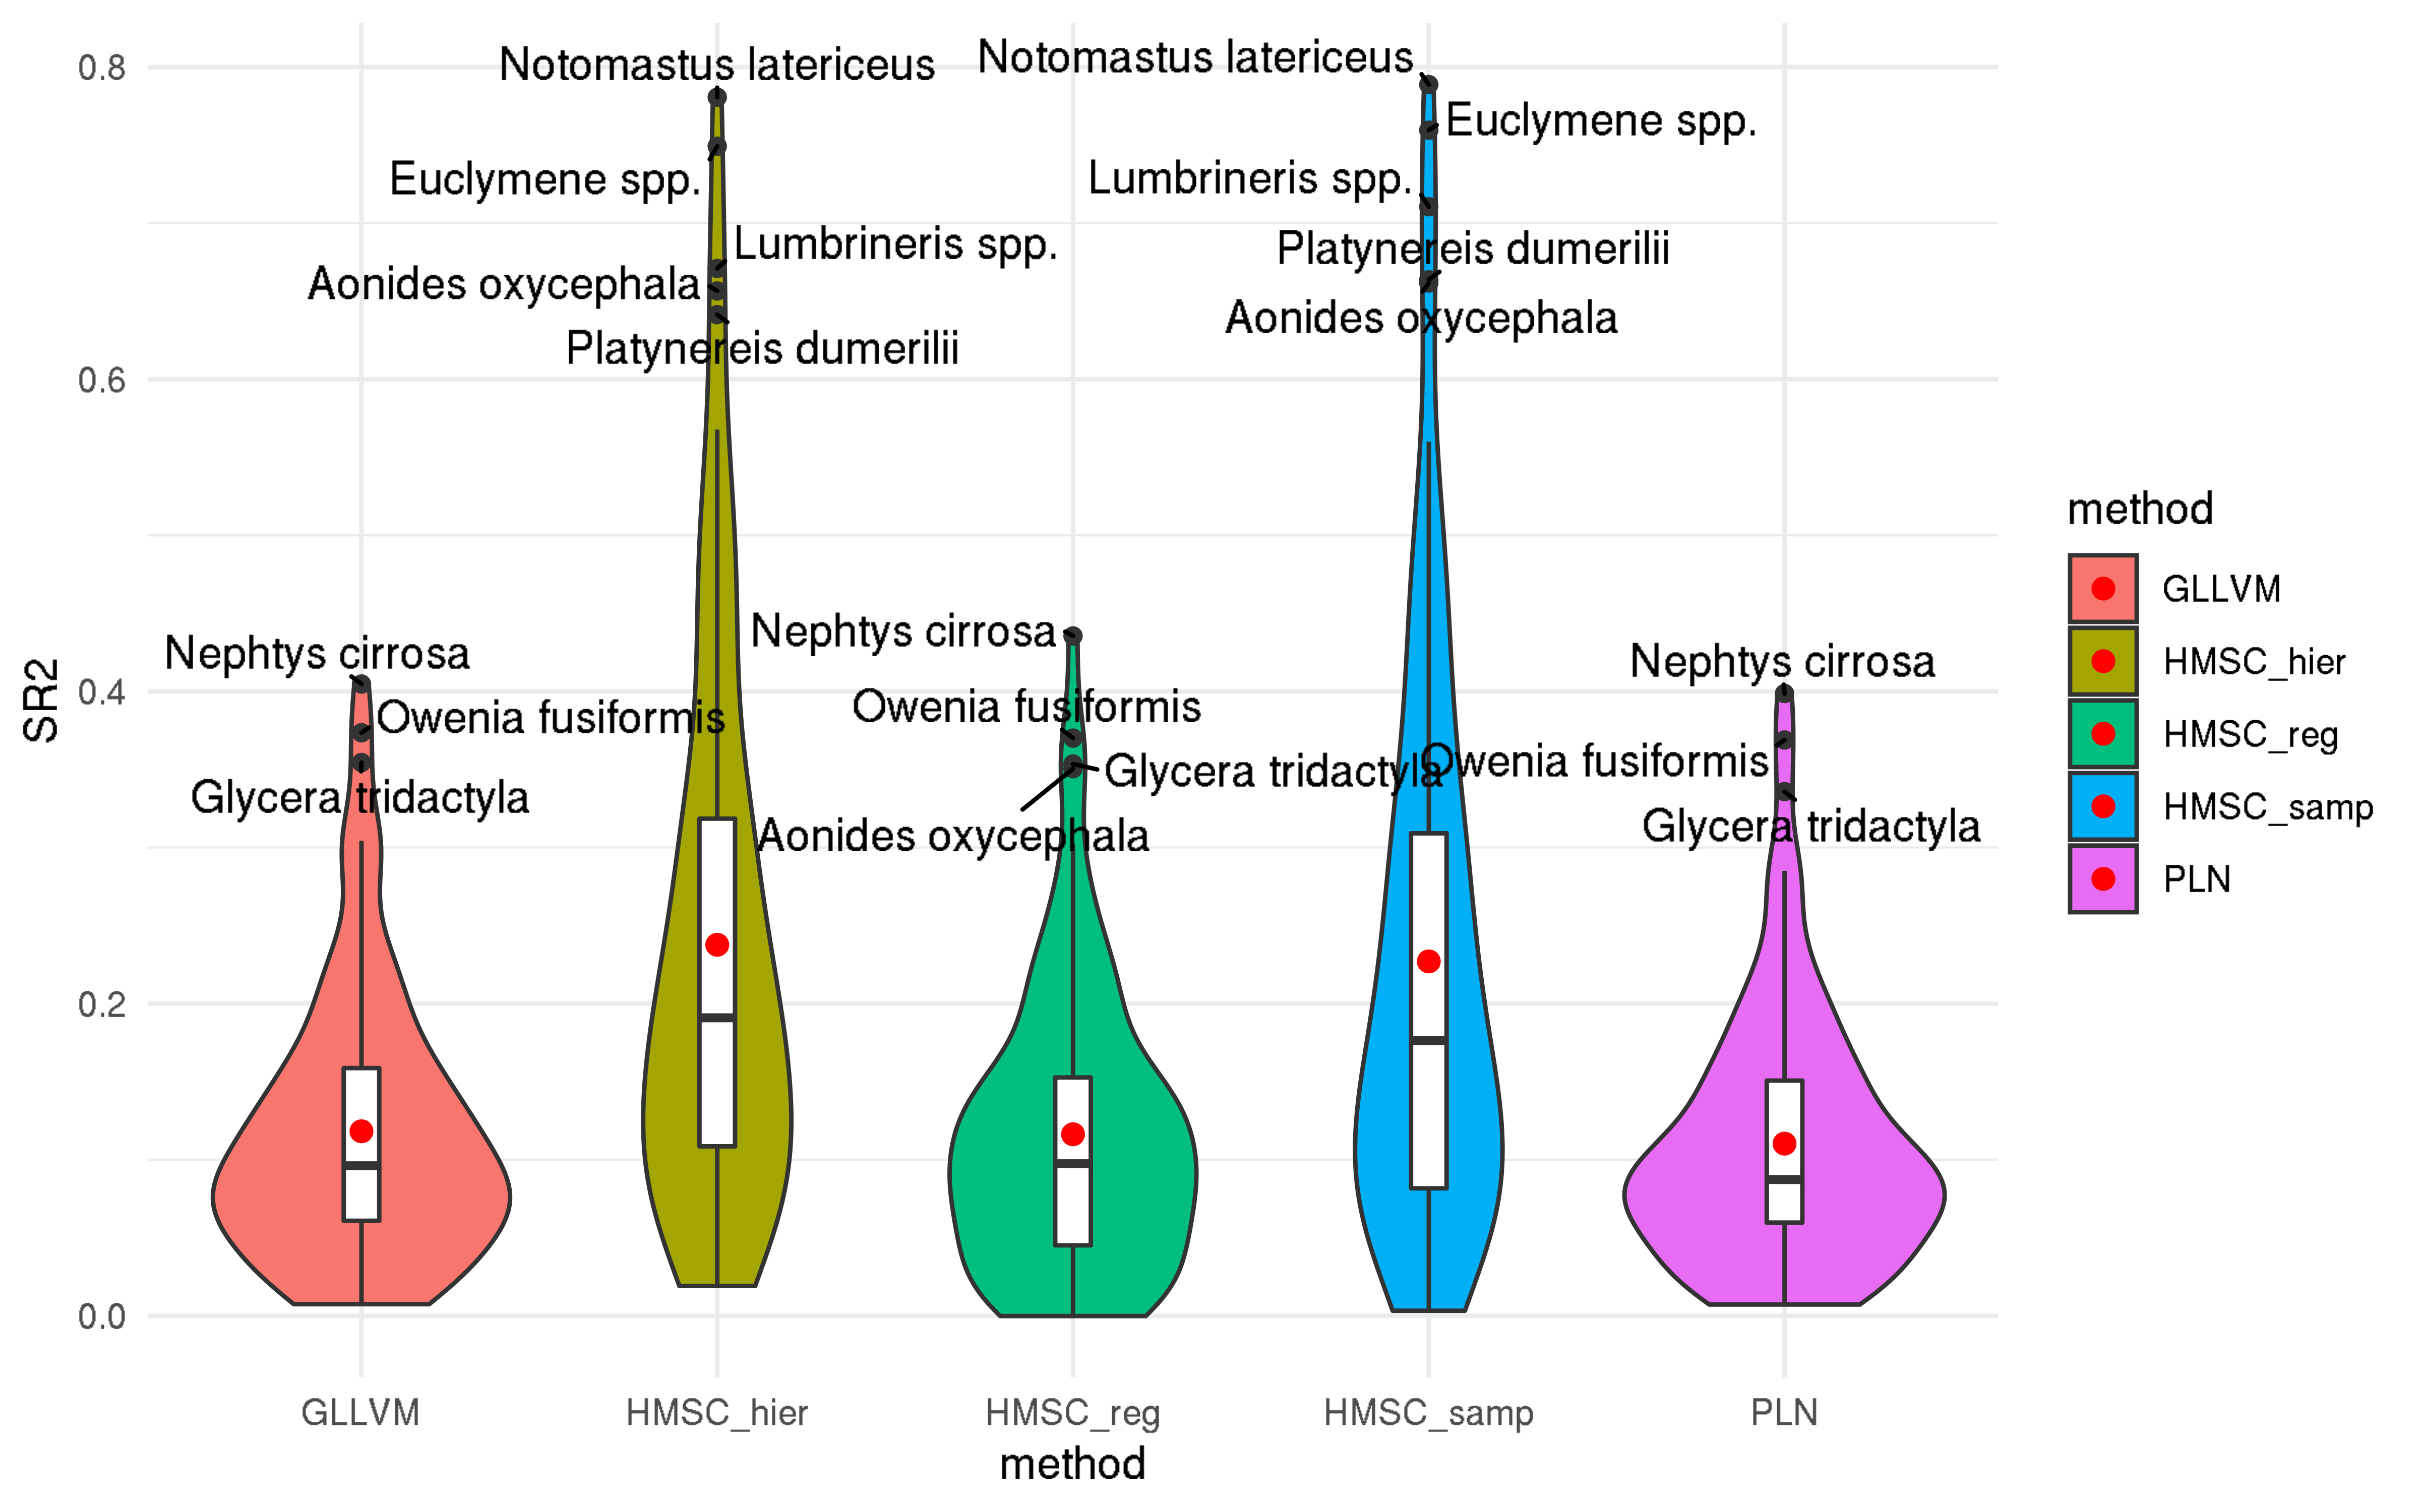
\includegraphics{figures/SR2-density-method-2.png}
\caption{Distribution du SR\textsuperscript{2} de l'abondance des 92
taxa de polychètes pour chaque modèle. Les points rouges représentent la
valeur moyenne du \emph{SR\textsuperscript{2}} pour chaque modèle. Les
points noirs représentent les espèces ayant une valeur extrême de
SR\textsuperscript{2}.}\label{fig:SR2}
}
\end{figure}

\hypertarget{pruxe9diction-de-loccurrence-et-de-labondance}{%
\subsubsection{Prédiction de l'occurrence et de
l'abondance}\label{pruxe9diction-de-loccurrence-et-de-labondance}}

La validation croisée sur trois sites tests (exclus de l'apprentissage)
permet la comparaison du pouvoir prédictif des modèles en termes de
richesse spécifique et d'abondance, et ce sur les 8 années de suivis de
ces trois sites.

\hypertarget{abondance}{%
\paragraph{Abondance}\label{abondance}}

Aucun modèle ne parvient à prédire de manière satisfaisante l'abondance
des espèces à chaque site. Le modèle le moins mauvais est le modèle
\emph{HMSC\_hier} dont la plus faible valeur de \emph{RMSE} pour une
espèce est de 24 individus et la plus forte valeur de \emph{RMSE} est de
l'ordre de \(10^4\). En moyenne ce modèle présente un \emph{RMSE} de
l'ordre de \(3,63\times 10^3\). Bien que cette erreur moyenne soit
importante, elle est plus faible que celle des autres modèles (entre
\(6,53\times 10^3\) et \(1,09\times 10^{36}\)). Le modèle GLLVM apparaît
comme le moins fiable pour estimer l'abondance, avec une erreur minimale
de prédiction de l'ordre de \(10^31\).

\hypertarget{occurrence}{%
\paragraph{Occurrence}\label{occurrence}}

Si aucun modèle n'arrive pleinement à reproduire les richesses observées
aux sites de validation et leurs dynamiques temporelles
((\cref{fig:predoccbrt}, \cref{fig:predocccorr} et
\cref{fig:occpredtemp}), les prédictions de l'occurrence des espèces
semblent bien plus réalistes que celles concernant leur abondance.

\begin{figure}
\hypertarget{fig:predoccbrt}{%
\centering
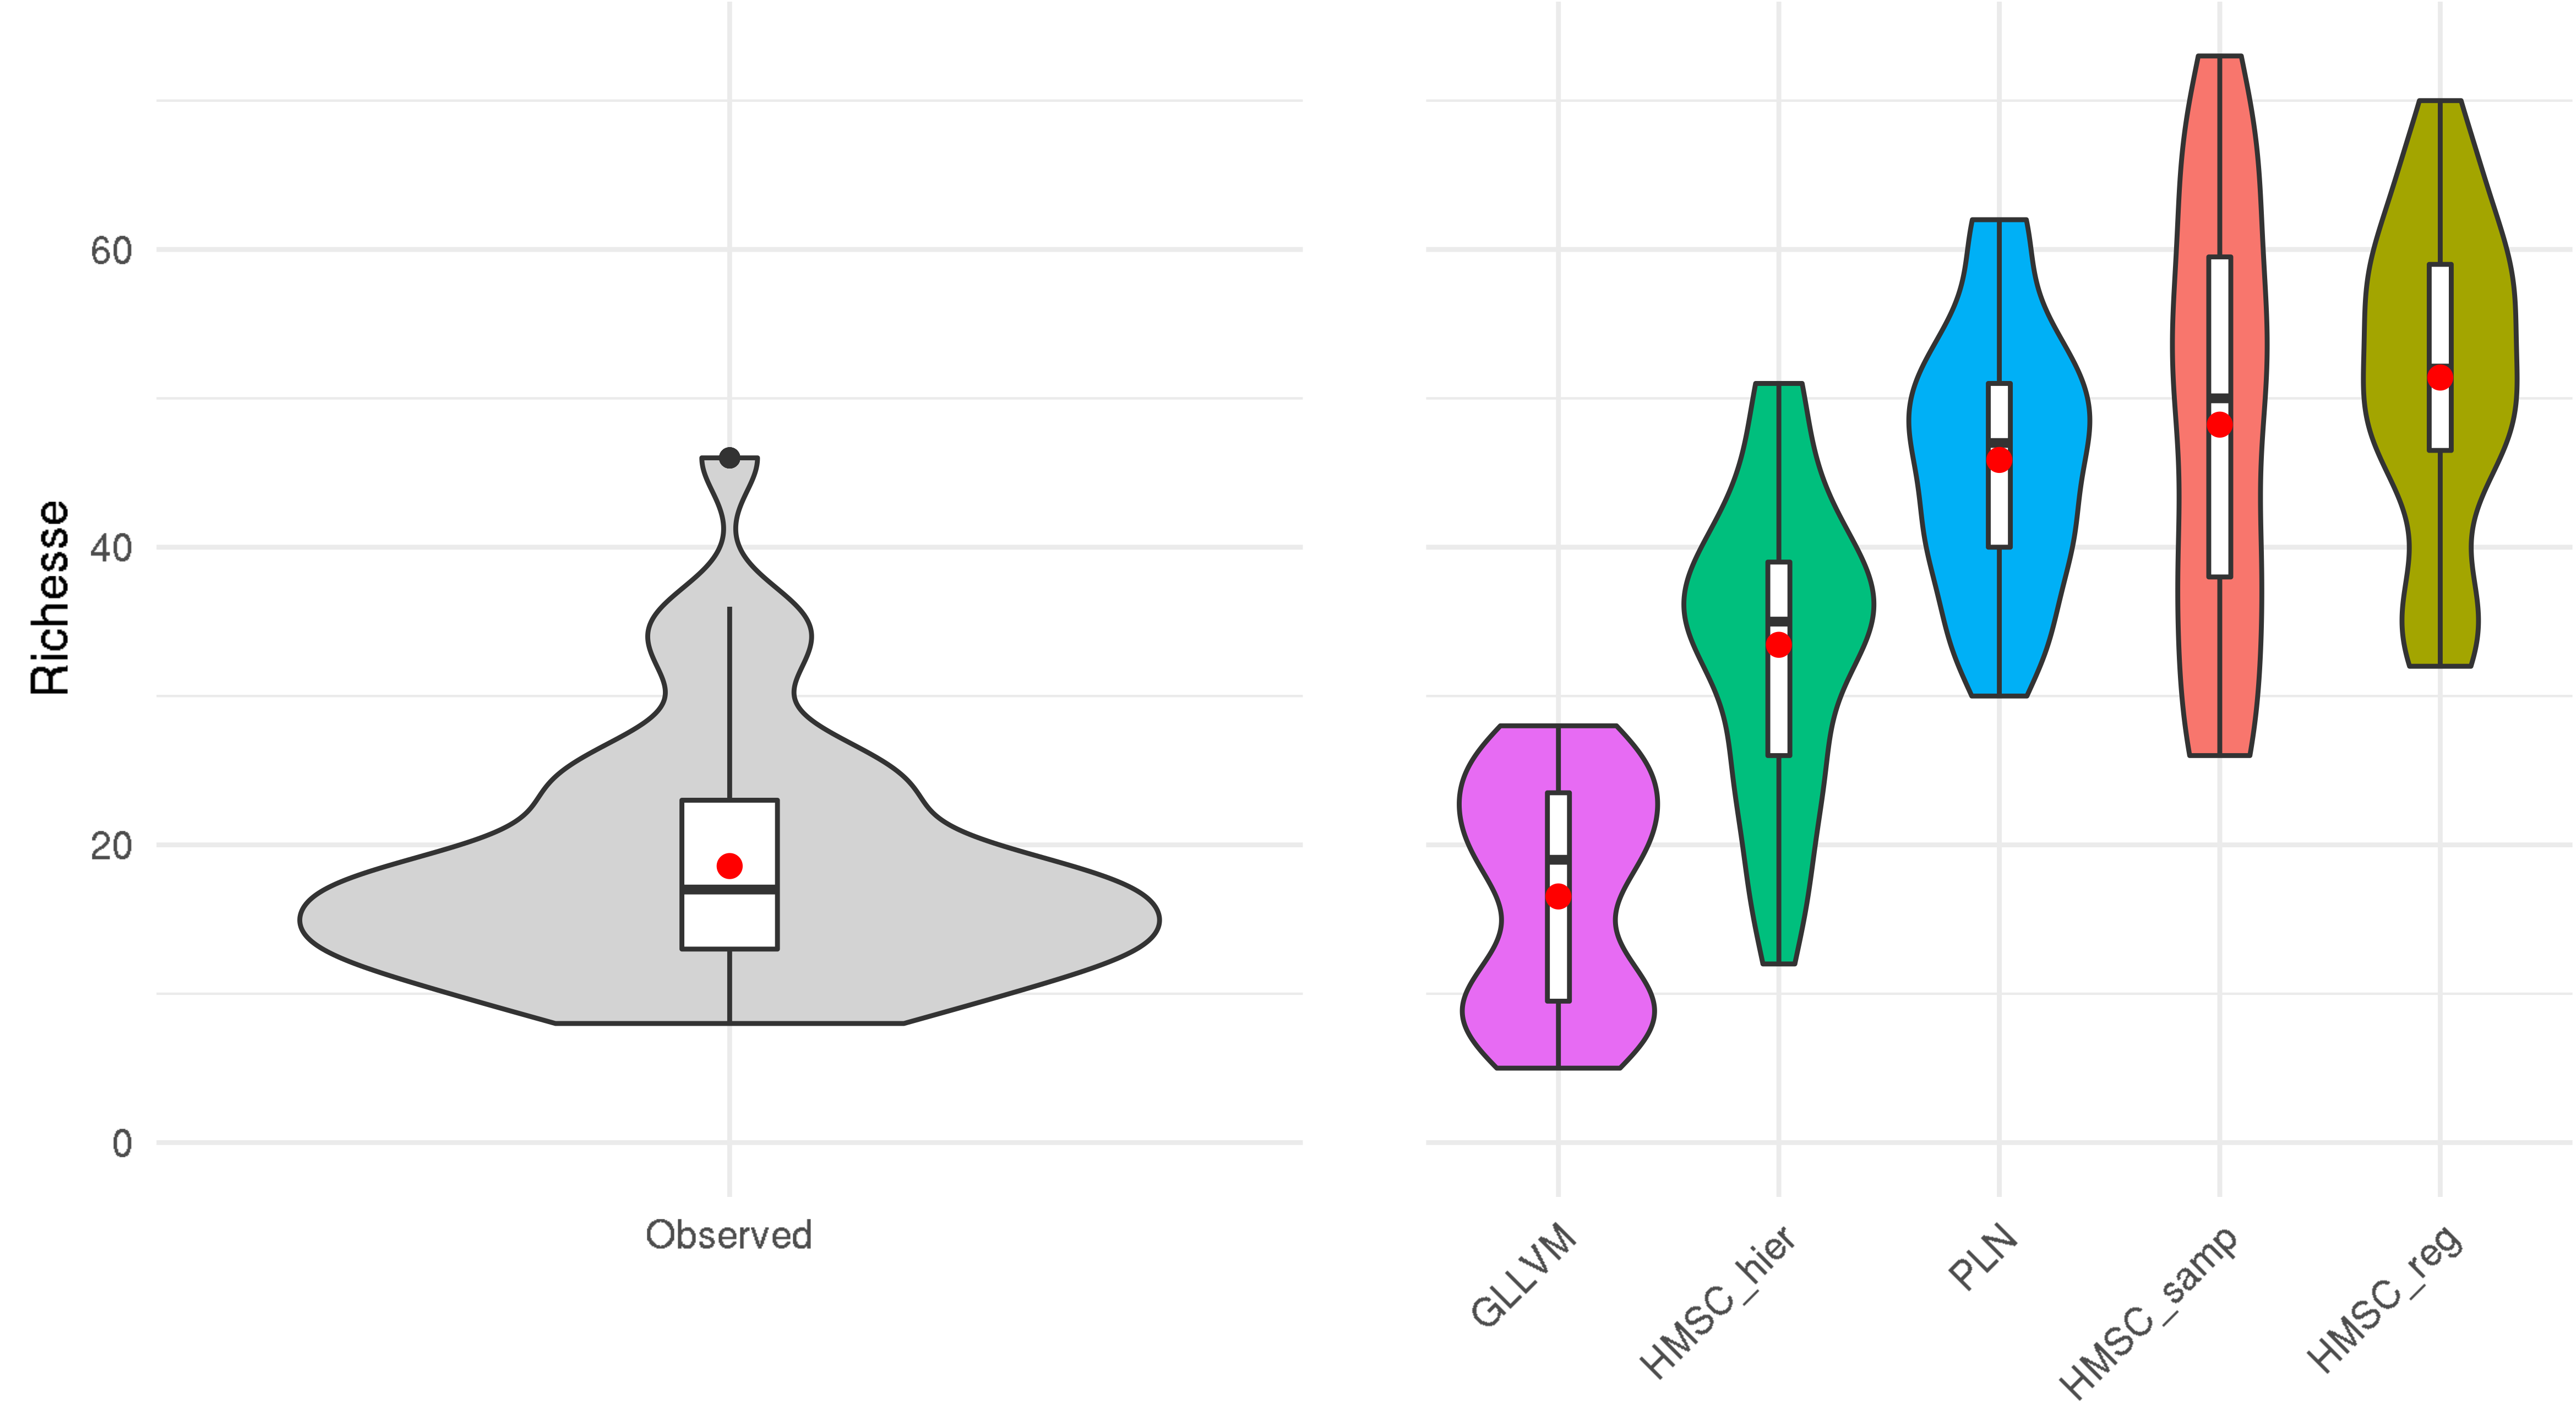
\includegraphics{figures/occurence_brt.png}
\caption{Variabilité spatiale et temporelle de la richesse spécifique
observée et prédite par les différentes méthodes de \emph{JSDM} pour les
3 sites de validation. Les points rouges correspondent à la richesse
moyenne des sites de validation.}\label{fig:predoccbrt}
}
\end{figure}

\begin{figure}
\hypertarget{fig:predocccorr}{%
\centering
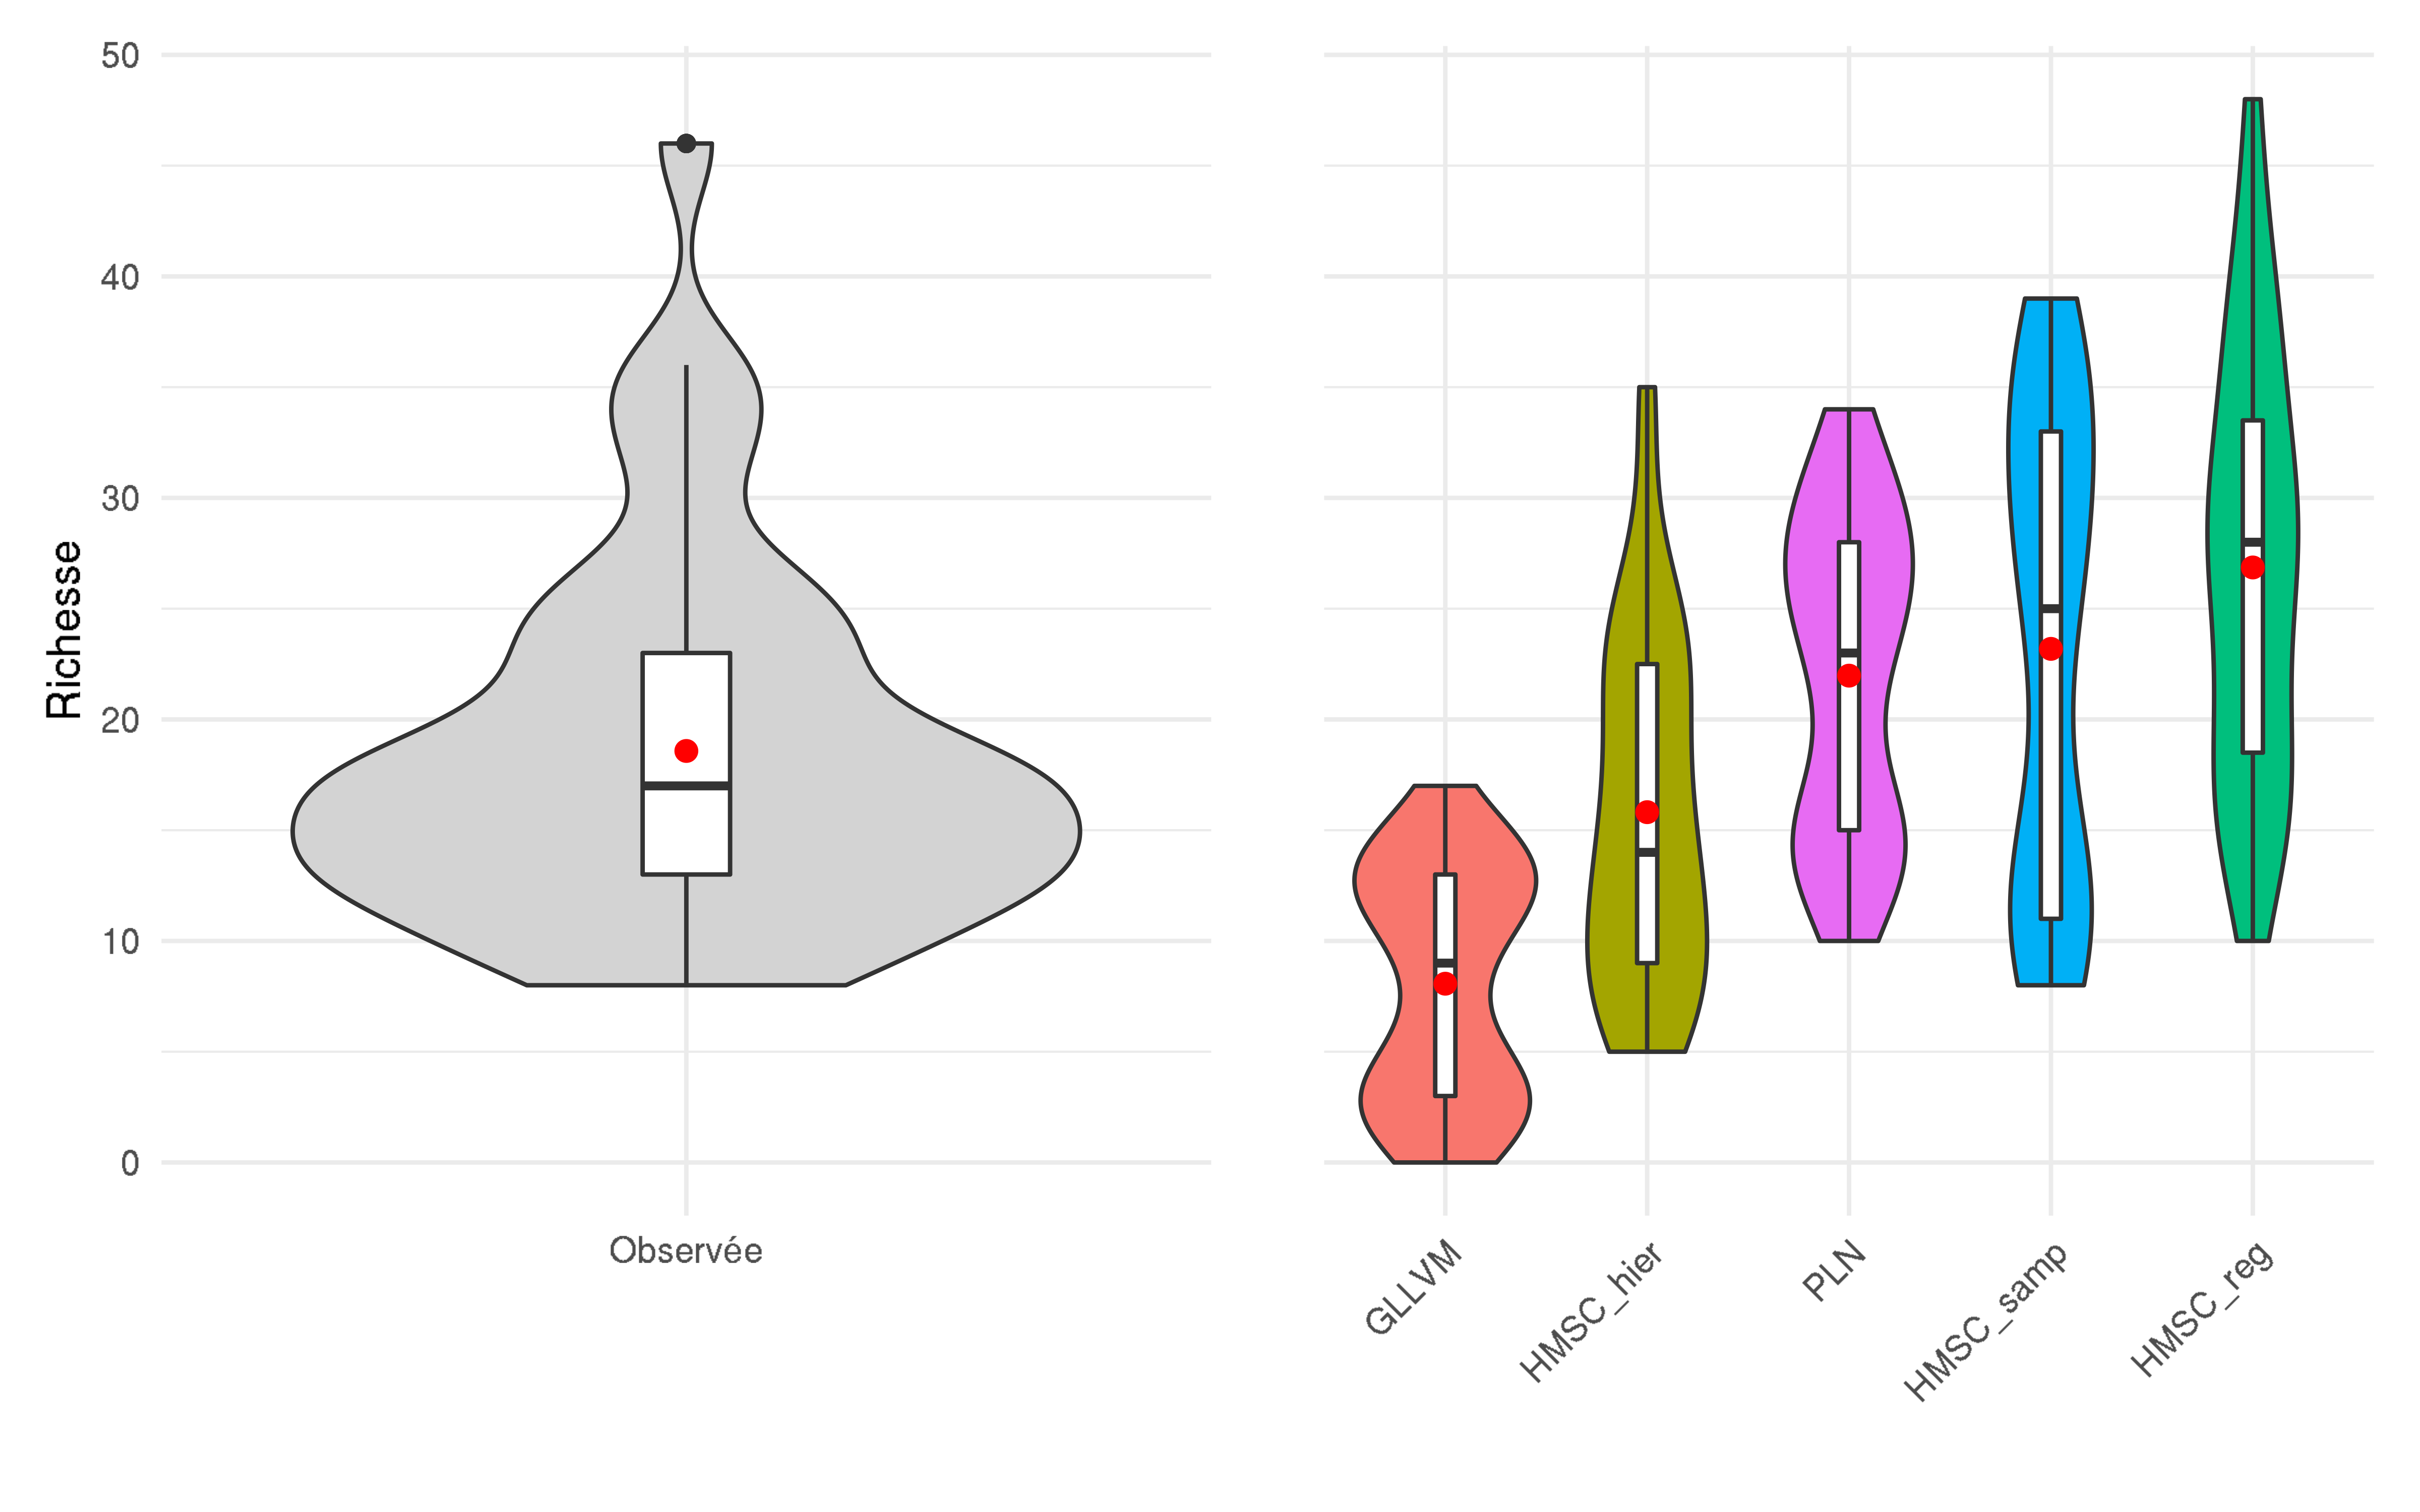
\includegraphics{figures/occurence_corr.png}
\caption{Variabilité spatiale et temporelle de la richesse spécifique
observée, corrigée par les seuils d'abondance et prédite par les
différentes méthodes de \emph{JSDM} pour les 3 sites de validation. Les
points rouges correspondent à la richesse moyenne des sites de
validation.}\label{fig:predocccorr}
}
\end{figure}

La richesse moyenne observée aux sites de validation est d'environ 20
espèces. Si l'on considère qu'une espèce est présente à partir du moment
où son abondance prédite est supérieure à 0, \emph{GLLVM} est le modèle
dont la richesse prédite est la plus proche de celle observée, en ayant
toutefois tendance à sous-estimer la richesse moyenne
(\cref{fig:predoccbrt}, \cref{fig:predocccorr} et
\cref{fig:occpredtemp}). Cette sous-estimation est encore plus prégnante
lorsqu'on utilise un seuil d'abondance adapté pour estimer l'occurrence
des espèces (\cref{fig:occpredtemp}). Au contraire, \emph{PLN},
\emph{GLLVM} et \emph{HMSC\_samp} surestiment la richesse des
communautés avec une richesse moyenne deux fois supérieure à celle
observée si l'on convertit directement l'abondance prédite des espèces
en présence/absence, mais sont dans une gamme de richesse plus cohérente
lorsque l'approche par seuil est utilisée. Dans les deux approches,
\emph{HMSC\_hier} apparaît comme la meilleure méthode pour estimer
l'occurrence des espèces et prédire la richesse des assemblages de
polychètes. Sans définir de seuil spécifique de présence effective, le
\emph{RMSE} indique que l'erreur sur la prédiction de la richesse
spécifique est finalement relativement faible pour l'ensemble des
modèles (\cref{tbl:RMSEocc}). Le \emph{RMSE} médian est de 7 pour le
modèle \emph{GLLVM} et de 16 pour le modèle \emph{HMSC\_hier}. Mais ce
\emph{RMSE} \emph{médian} est près de deux fois plus élevées pour les
modèles \emph{PLN}, \emph{HMSC\_samp} et \emph{HMSC\_reg}.

{\small
\begin{longtable}[]{@{}lllllll@{}}
\caption{Statistiques descriptives du \emph{RMSE} de la richesse
spécifique par modèle. Les modèles sont classés par ordre croissant de
\emph{RMSE} maximal. Q1 et Q3 représentent respectivement le premier et
troisième quartile du \emph{RMSE} de chaque modèle.
\label{tbl:RMSEocc}}\tabularnewline
\toprule
Method & Min & Q1 & Median & Moy & Q3 & Max\tabularnewline
\midrule
\endfirsthead
\toprule
Method & Min & Q1 & Median & Moy & Q3 & Max\tabularnewline
\midrule
\endhead
\emph{GLLVM} & \(0\) & \(3,0\) & \(7\) & \(7,63\) & \(10,0\) &
\(29\)\tabularnewline
\emph{HMSC\_hier} & \(1\) & \(11,5\) & \(16\) & \(15,37\) & \(20,0\) &
\(33\)\tabularnewline
\emph{PLN} & \(4\) & \(21,0\) & \(27\) & \(27,28\) & \(33,0\) &
\(51\)\tabularnewline
\emph{HMSC\_reg} & \(6\) & \(25,0\) & \(33\) & \(32,84\) & \(40,5\) &
\(56\)\tabularnewline
\emph{HMSC\_samp} & \(4\) & \(18,5\) & \(30\) & \(29,65\) & \(38,5\) &
\(62\)\tabularnewline
\bottomrule
\end{longtable}}\FloatBarrier


Les modèles prédisent correctement la variabilité de la richesse
inter-site en trouvant tous l'ordre de grandeur de la richesse
spécifique pour chaque site (\cref{fig:occpredtemp}). Les modèles
prédisent mieux la richesse spécifique dans les herbiers que dans les
plages de sable. \emph{HMSC\_hier} est le modèle qui prédit le mieux la
variabilité de la richesse spécifique. Ce modèle arrive à également
prédire les fluctuations temporelles, notamment la diminution de la
richesse spécifique observée pour les herbiers en 2009.

\begin{figure}
\hypertarget{fig:occpredtemp}{%
\centering
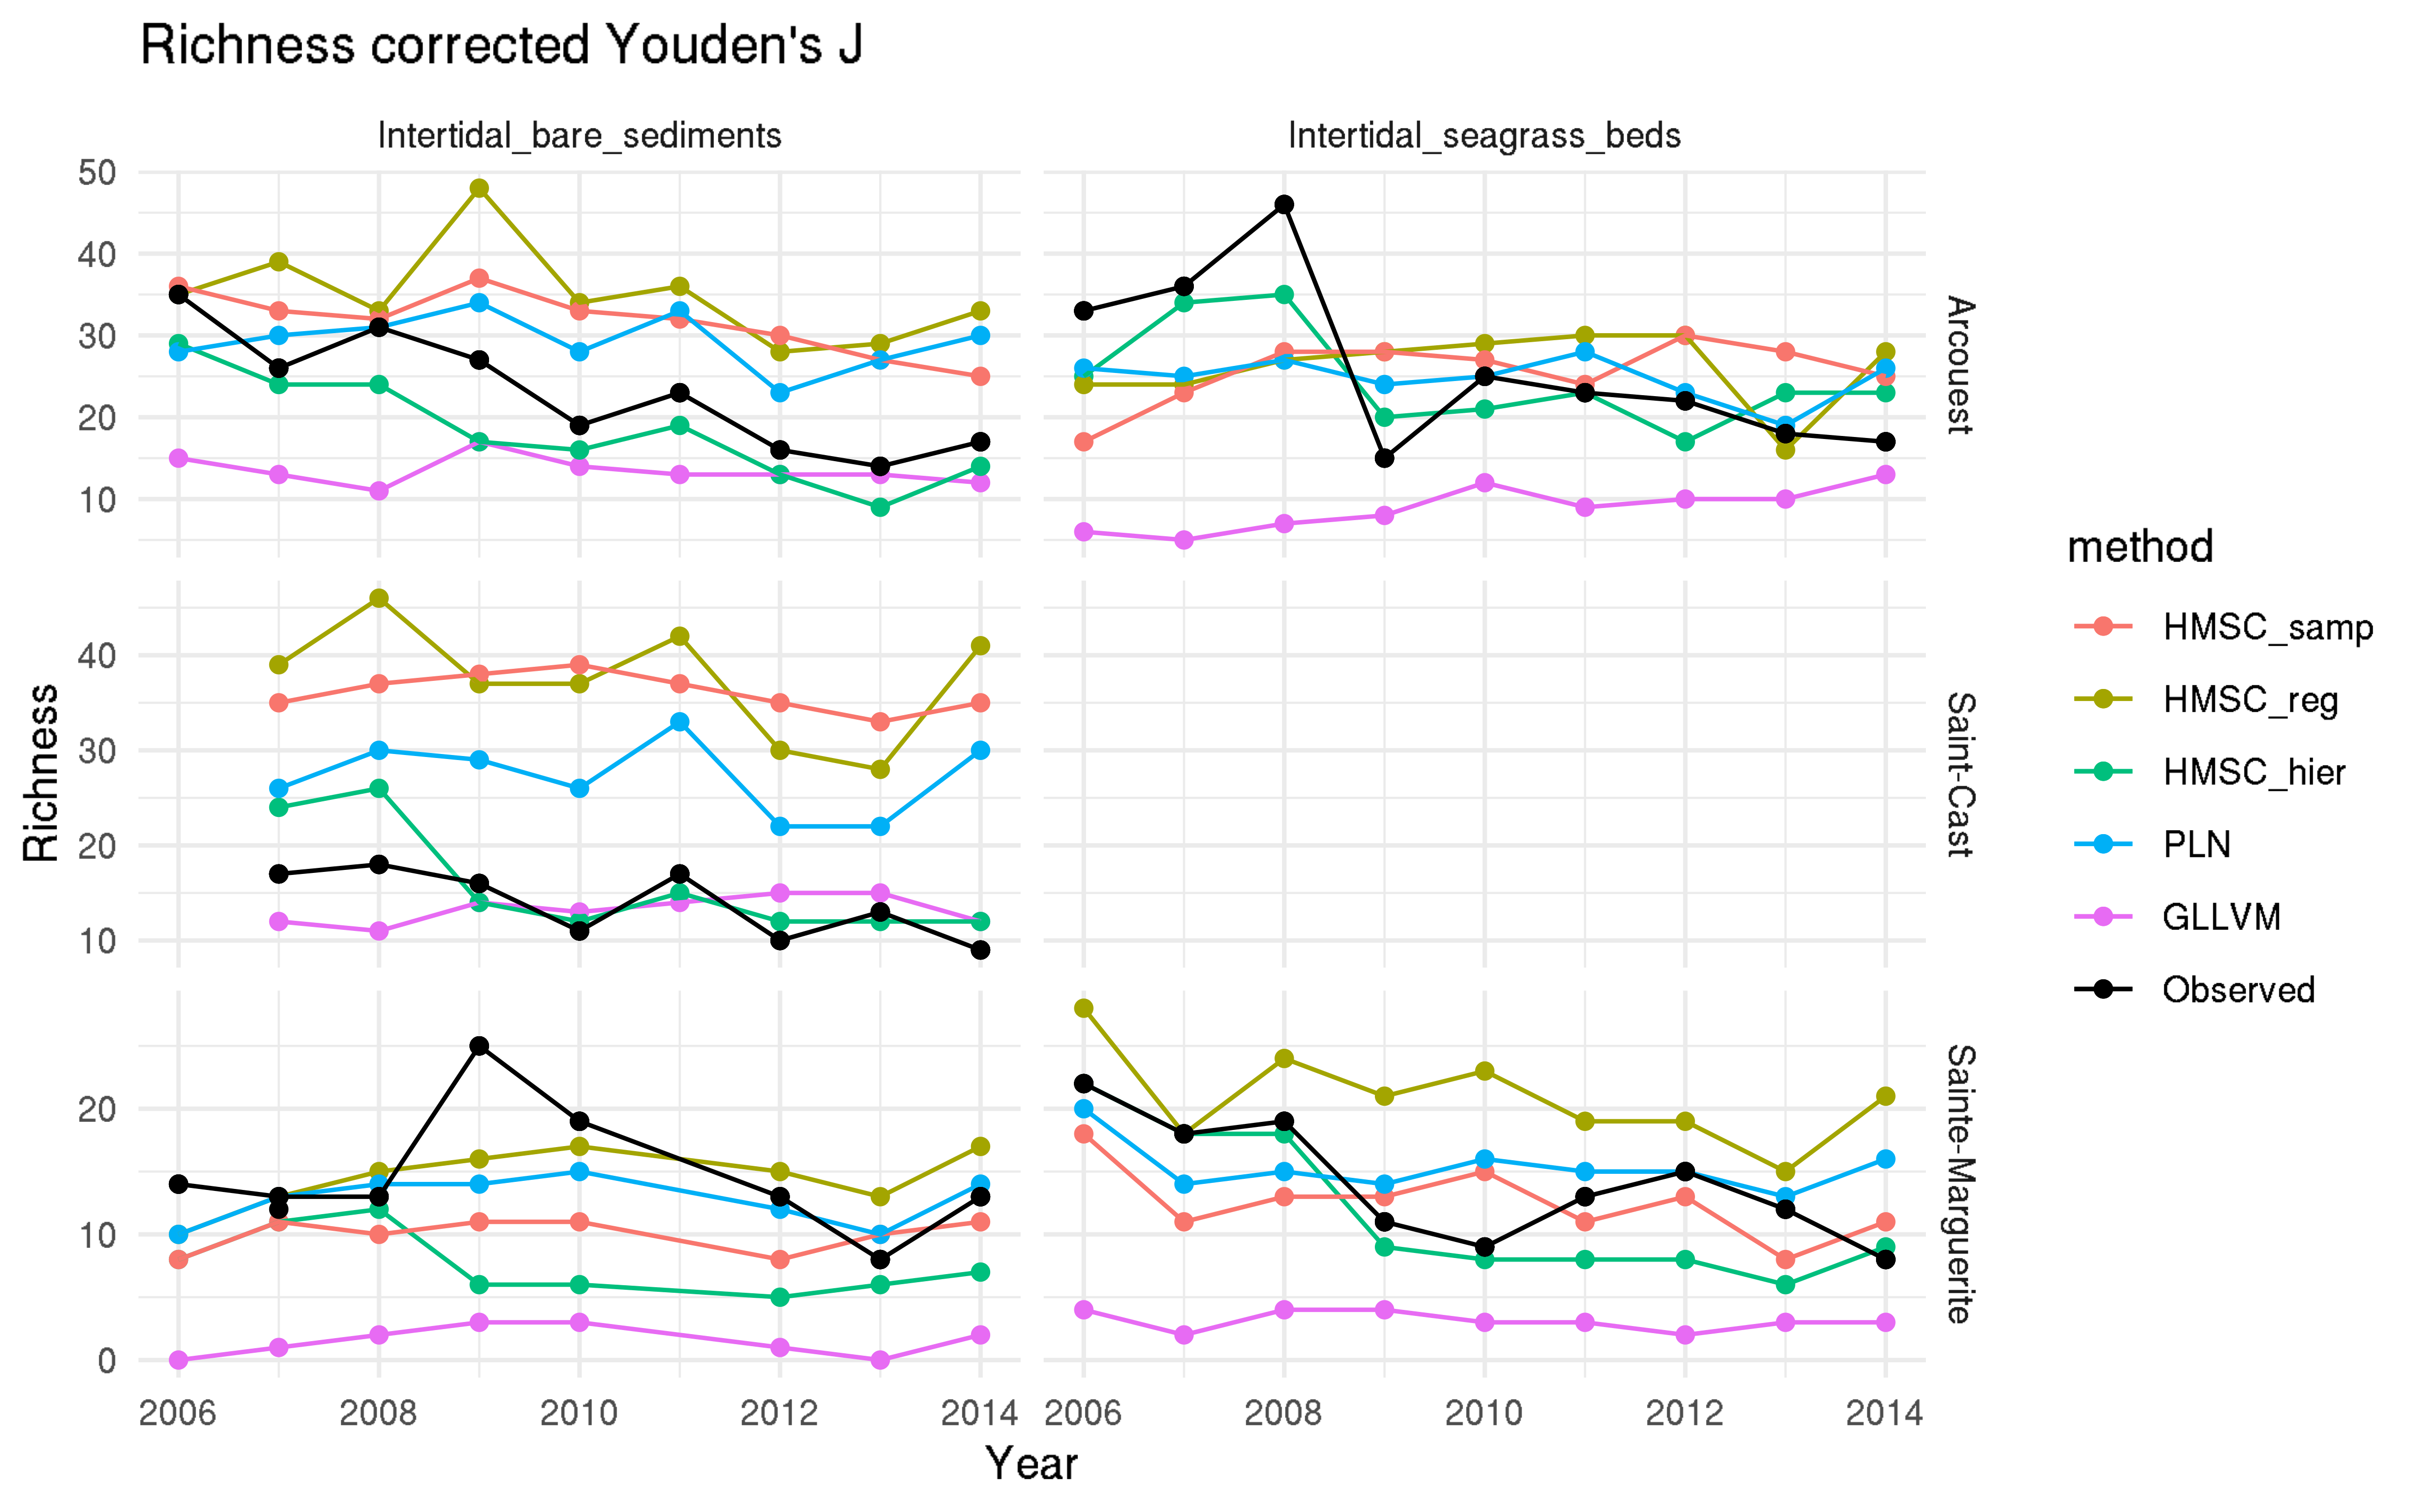
\includegraphics{figures/roc-richness-prediction-3.png}
\caption{Variabilité spatio-temporelle de la prédiction de la diversité
spécifique des communautés de polychètes selon les différentes méthodes
de \emph{JSDM}. L'occurrence prédite est basée sur des seuils de
probabilité spécifiques à chaque taxon.}\label{fig:occpredtemp}
}
\end{figure}

\hypertarget{effets-de-lenvironnement}{%
\subsection{Effets de l'environnement}\label{effets-de-lenvironnement}}

Les effets des variables environnementales sur l'abondance prédite des
différents taxa sont globalement similaires à travers les différents
modèles (\cref{fig:effectenv}). Dans la \cref{fig:effectenv} les
variables environnementales sont ordonnées par proportion décroissante
de variances expliquée. Ainsi, des variables mesurées à l'échelle du
site comme l'exposition (Fetch) ou la vitesse moyenne du courant
expliquent une plus grande part de variance dans l'abondance des espèces
que les variables sédimentologiques comme l'indice de Trask ou la
concentration en vase mesurée à une échelle plus locale
(\cref{fig:varpartreg} à \ref{fig:varparthier} en annexe). L'analyse de
cette figure par les experts benthologues a aussi mis en lumière que ces
espèces étaient toutes majoritairement inféodées à des environnements de
sables fins, ce qui tend à corroborer les effets positifs du Trask
observés dans la majorité des modèles, sauf \emph{HMSC\_hier}. Dans
l'ensemble, les facteurs aléatoires sont ceux qui expliquent le plus de
la variation des espèces, notamment pour celles les mieux expliquées
(Figure 1 à 3 en annexe). La façon d'implémenter ces effets aléatoires
apparaît donc critique, d'autant que dans HMSC ils influencent
grandement les coefficients estimés (Figure 5).

Pour tous les modèles, l'effet des variables environnementales est assez
net pour les espèces les mieux expliquées (15 premières en partant du
haut) et devient moins marqué quand il s'agit d'expliquer l'abondance
des espèces les moins bien expliquées (espèces qui se trouvent dans le
tiers inférieur de la \cref{fig:effectenv}). De plus, tous les modèles
montrent un effet positif pour la variable Trask (plus le sédiment est
bien trié plus les espèces sont abondantes), à l'exception du modèle
\emph{HMSC\_hier}. Avec l'inclusion des effets aléatoire sites, habitats
et années, le modèle \emph{HMSC\_hier} montre à l'inverse un effet
faiblement négatif, voire négatif, sur l'abondance des espèces. Le
modèle \emph{HMSC\_hier} est ainsi celui qui se différencie le plus en
termes de coefficients estimés, ce qui semble en lien avec la part de
variance importante expliquée par l'ajout des facteurs aléatoires
(\cref{fig:varpartreg} à \ref{fig:varparthier}).

\begin{figure}
\hypertarget{fig:effectenv}{%
\centering
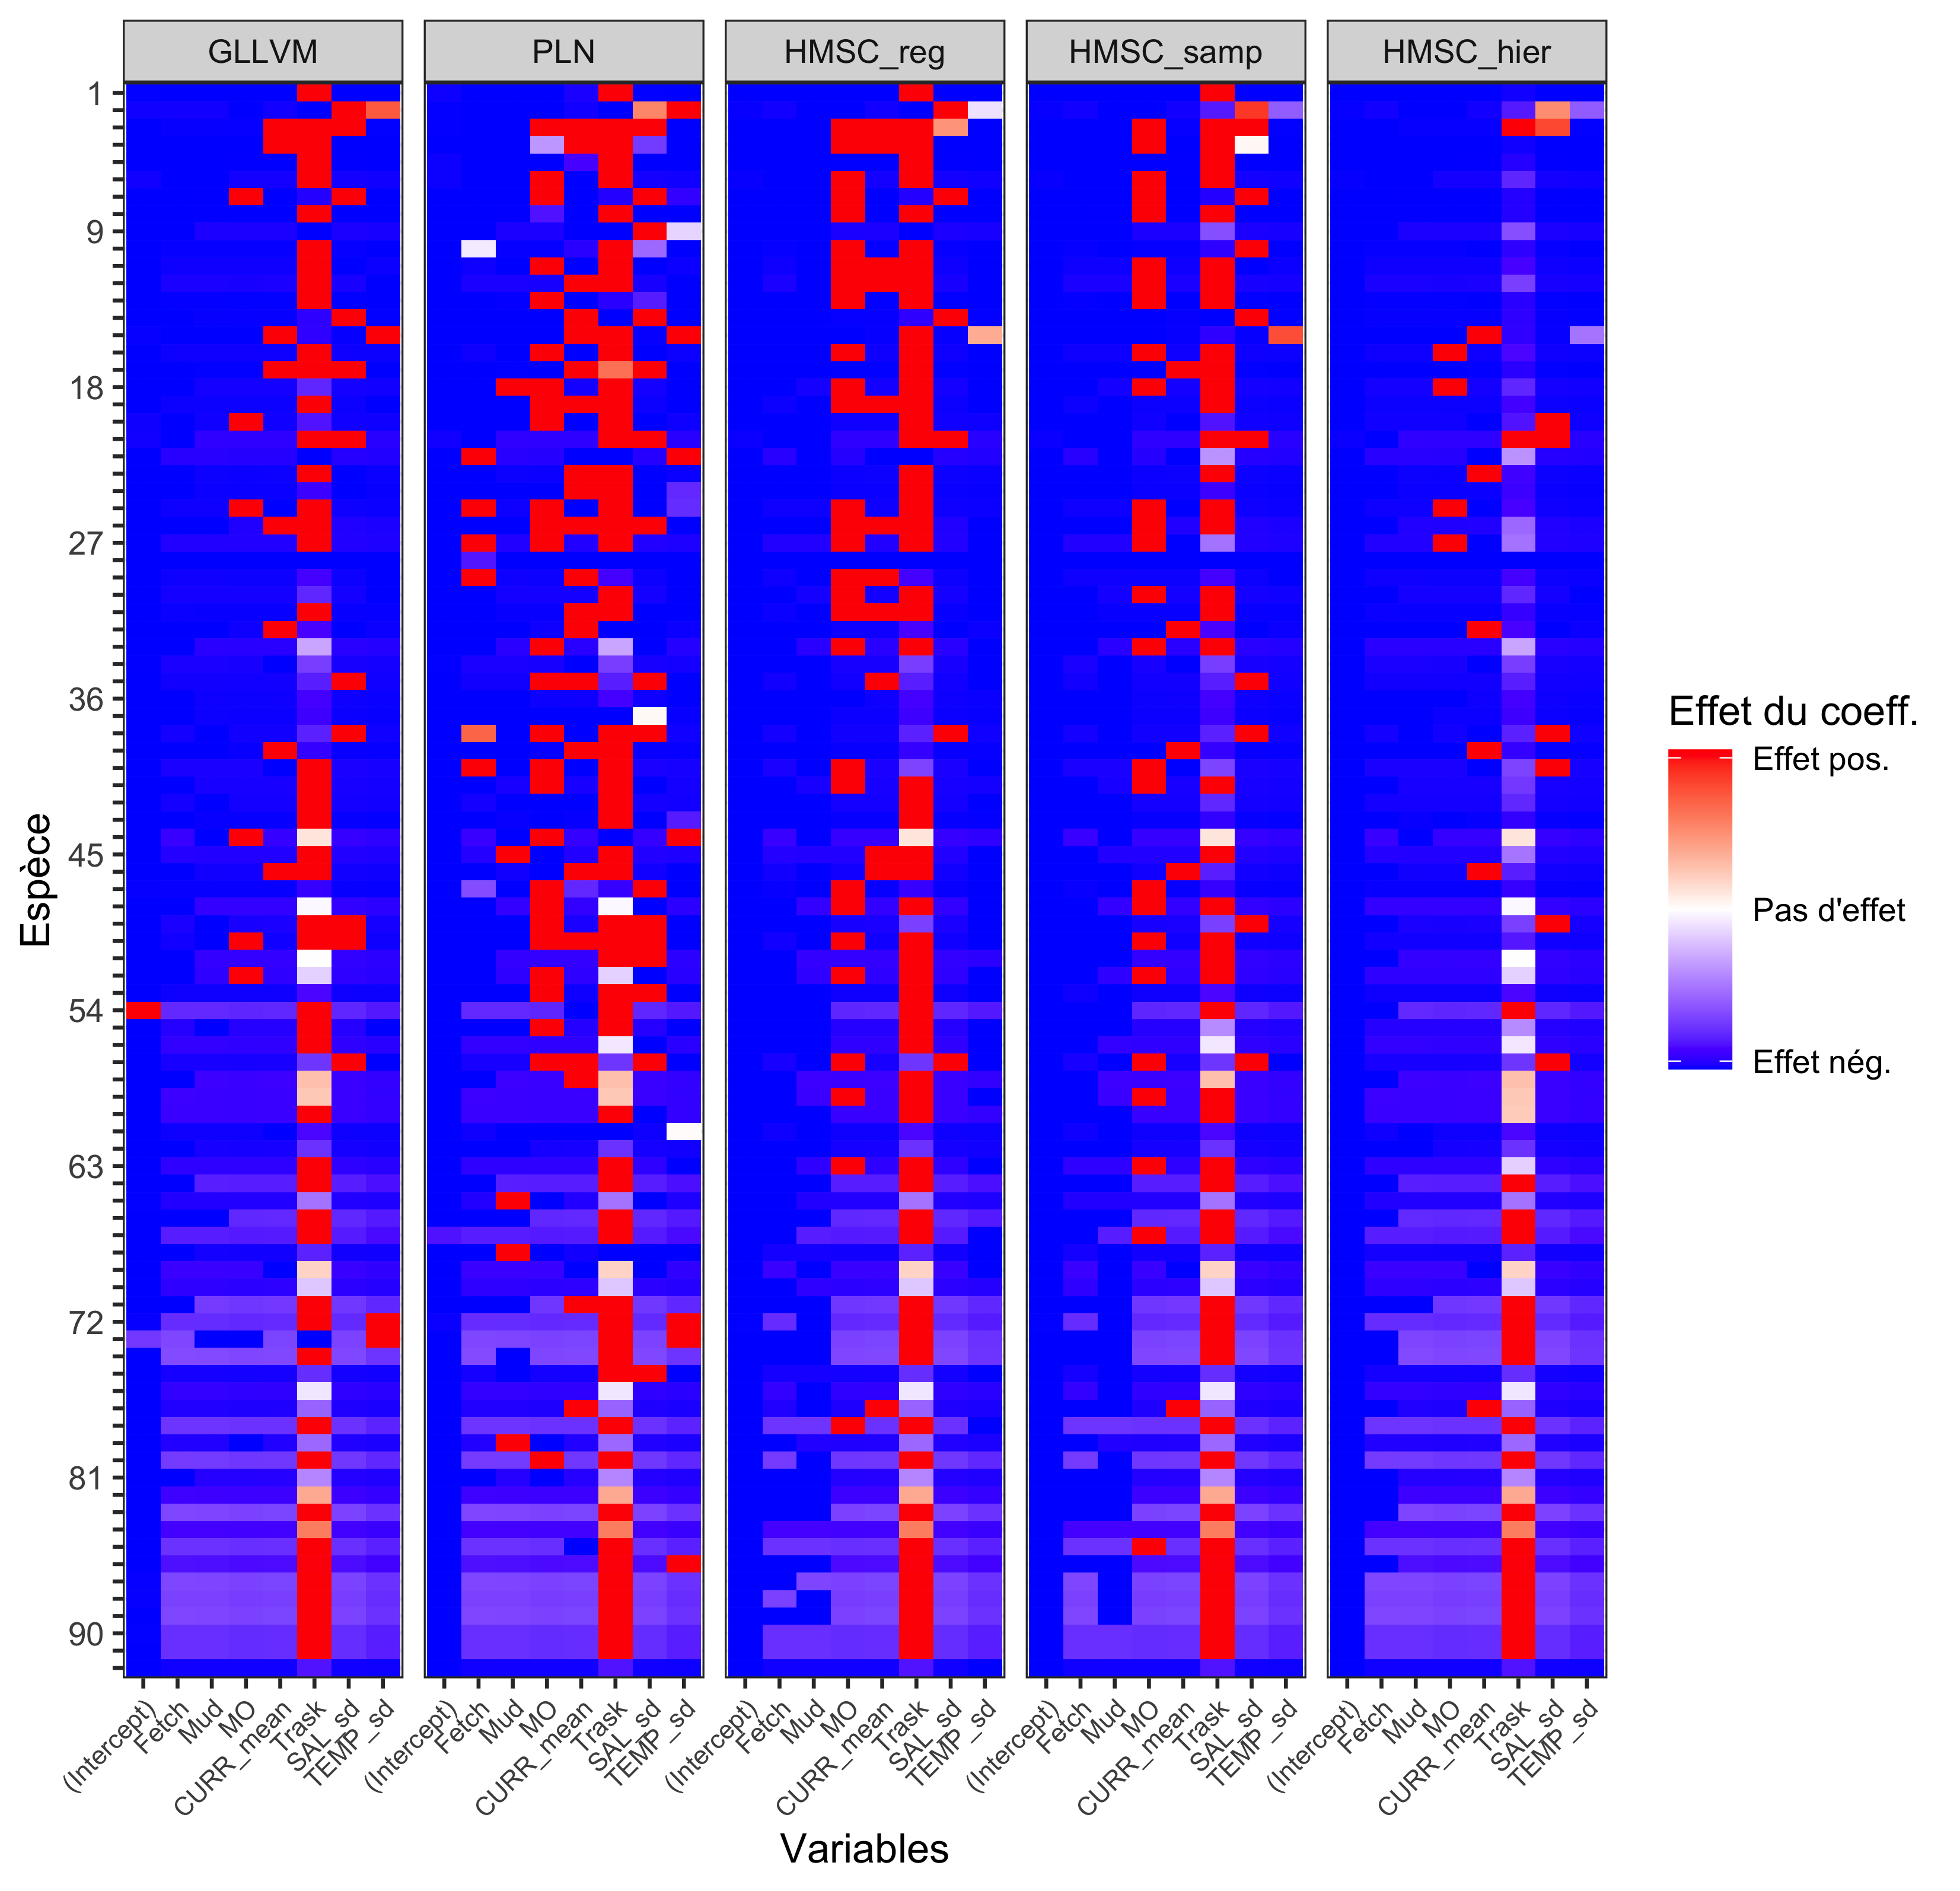
\includegraphics{figures/effect_env.png}
\caption{Effets des variables environnementales sur l'abondance des
différentes espèces de polychètes. Les variables et les abondances sont
centrées et réduites. Les espèces sont ordonnées par \(SR^2\) moyen
décroissant. Les variables environnementales sont ordonnées par
proportion de variances expliquées décroissante (voir \cref{tbl:env}
pour leur description).}\label{fig:effectenv}
}
\end{figure}

\hypertarget{ruxe9seaux-reconstruits}{%
\subsection{Réseaux reconstruits}\label{ruxe9seaux-reconstruits}}

\hypertarget{analyse-des-graphes}{%
\subsubsection{Analyse des graphes}\label{analyse-des-graphes}}

Tous les réseaux probabilistes reconstruits présentent le même nombre de
liens 182 et globalement, il y a peu de différence notable dans la
structure des réseaux inférés par les différents modèles
(\cref{tbl:metrics}\emph{). L'écart-type du nombre de liens est
légèrement plus important pour les effets aléatoires année et habitat du
modèle }HMSC\_hier* , mais reste dans des ordres de grandeur similaires
à ceux des autres modèles. La connectance , qui peut en théorie varier
entre 0 et 1, est quasiment identique pour tous les modèles et apparaît
extrêmement faible. L'imbrication des réseaux est aussi quasi nulle et
similaire sur l'ensemble des modèles.

{\small
\begin{longtable}[]{@{}lllr@{}}
\caption{Métrique des réseaux d'interactions reconstruits. \(\sigma_l\)
représente l'écart-type du nombre de liens. \(C\), Connectance.
\(\eta\), imbrication des réseaux trophiques.
\label{tbl:metrics}}\tabularnewline
\toprule
Méthode & \(\sigma_l\) & \(C\) & \(\eta\)\tabularnewline
\midrule
\endfirsthead
\toprule
Méthode & \(\sigma_l\) & \(C\) & \(\eta\)\tabularnewline
\midrule
\endhead
\emph{HMSC\_samp} & \(12,70\) & \(0,022\) & \(0,03\)\tabularnewline
\emph{HMSC\_hier\_annee} & \(13,10\) & \(0,021\) &
\(0,03\)\tabularnewline
\emph{HMSC\_hier\_site} & \(12,46\) & \(0,021\) &
\(0,03\)\tabularnewline
\emph{HMSC\_hier\_habitat} & \(13,11\) & \(0,021\) &
\(0,03\)\tabularnewline
\emph{GLLVM} & \(12,51\) & \(0,021\) & \(0.04\)\tabularnewline
\emph{PLN} & \(12,60\) & \(0,022\) & \(0.04\)\tabularnewline
\bottomrule
\end{longtable}}\FloatBarrier


Le réseau moyen reconstruit sur la base des corrélations résiduelles
entre taxons met en évidence un nombre restreint d'interactions
fortement probables (\cref{fig:meannet}) en corroborant les faibles
connectances estimées sur les réseaux individuels (\cref{tbl:metrics}).
Ainsi, beaucoup d'espèces ne semblent pas avoir de liens dans le réseau,
avec une majorité des interactions inférées ayant une probabilité
inférieure ou égale à \(0,2\).

\begin{figure}
\hypertarget{fig:meannet}{%
\centering
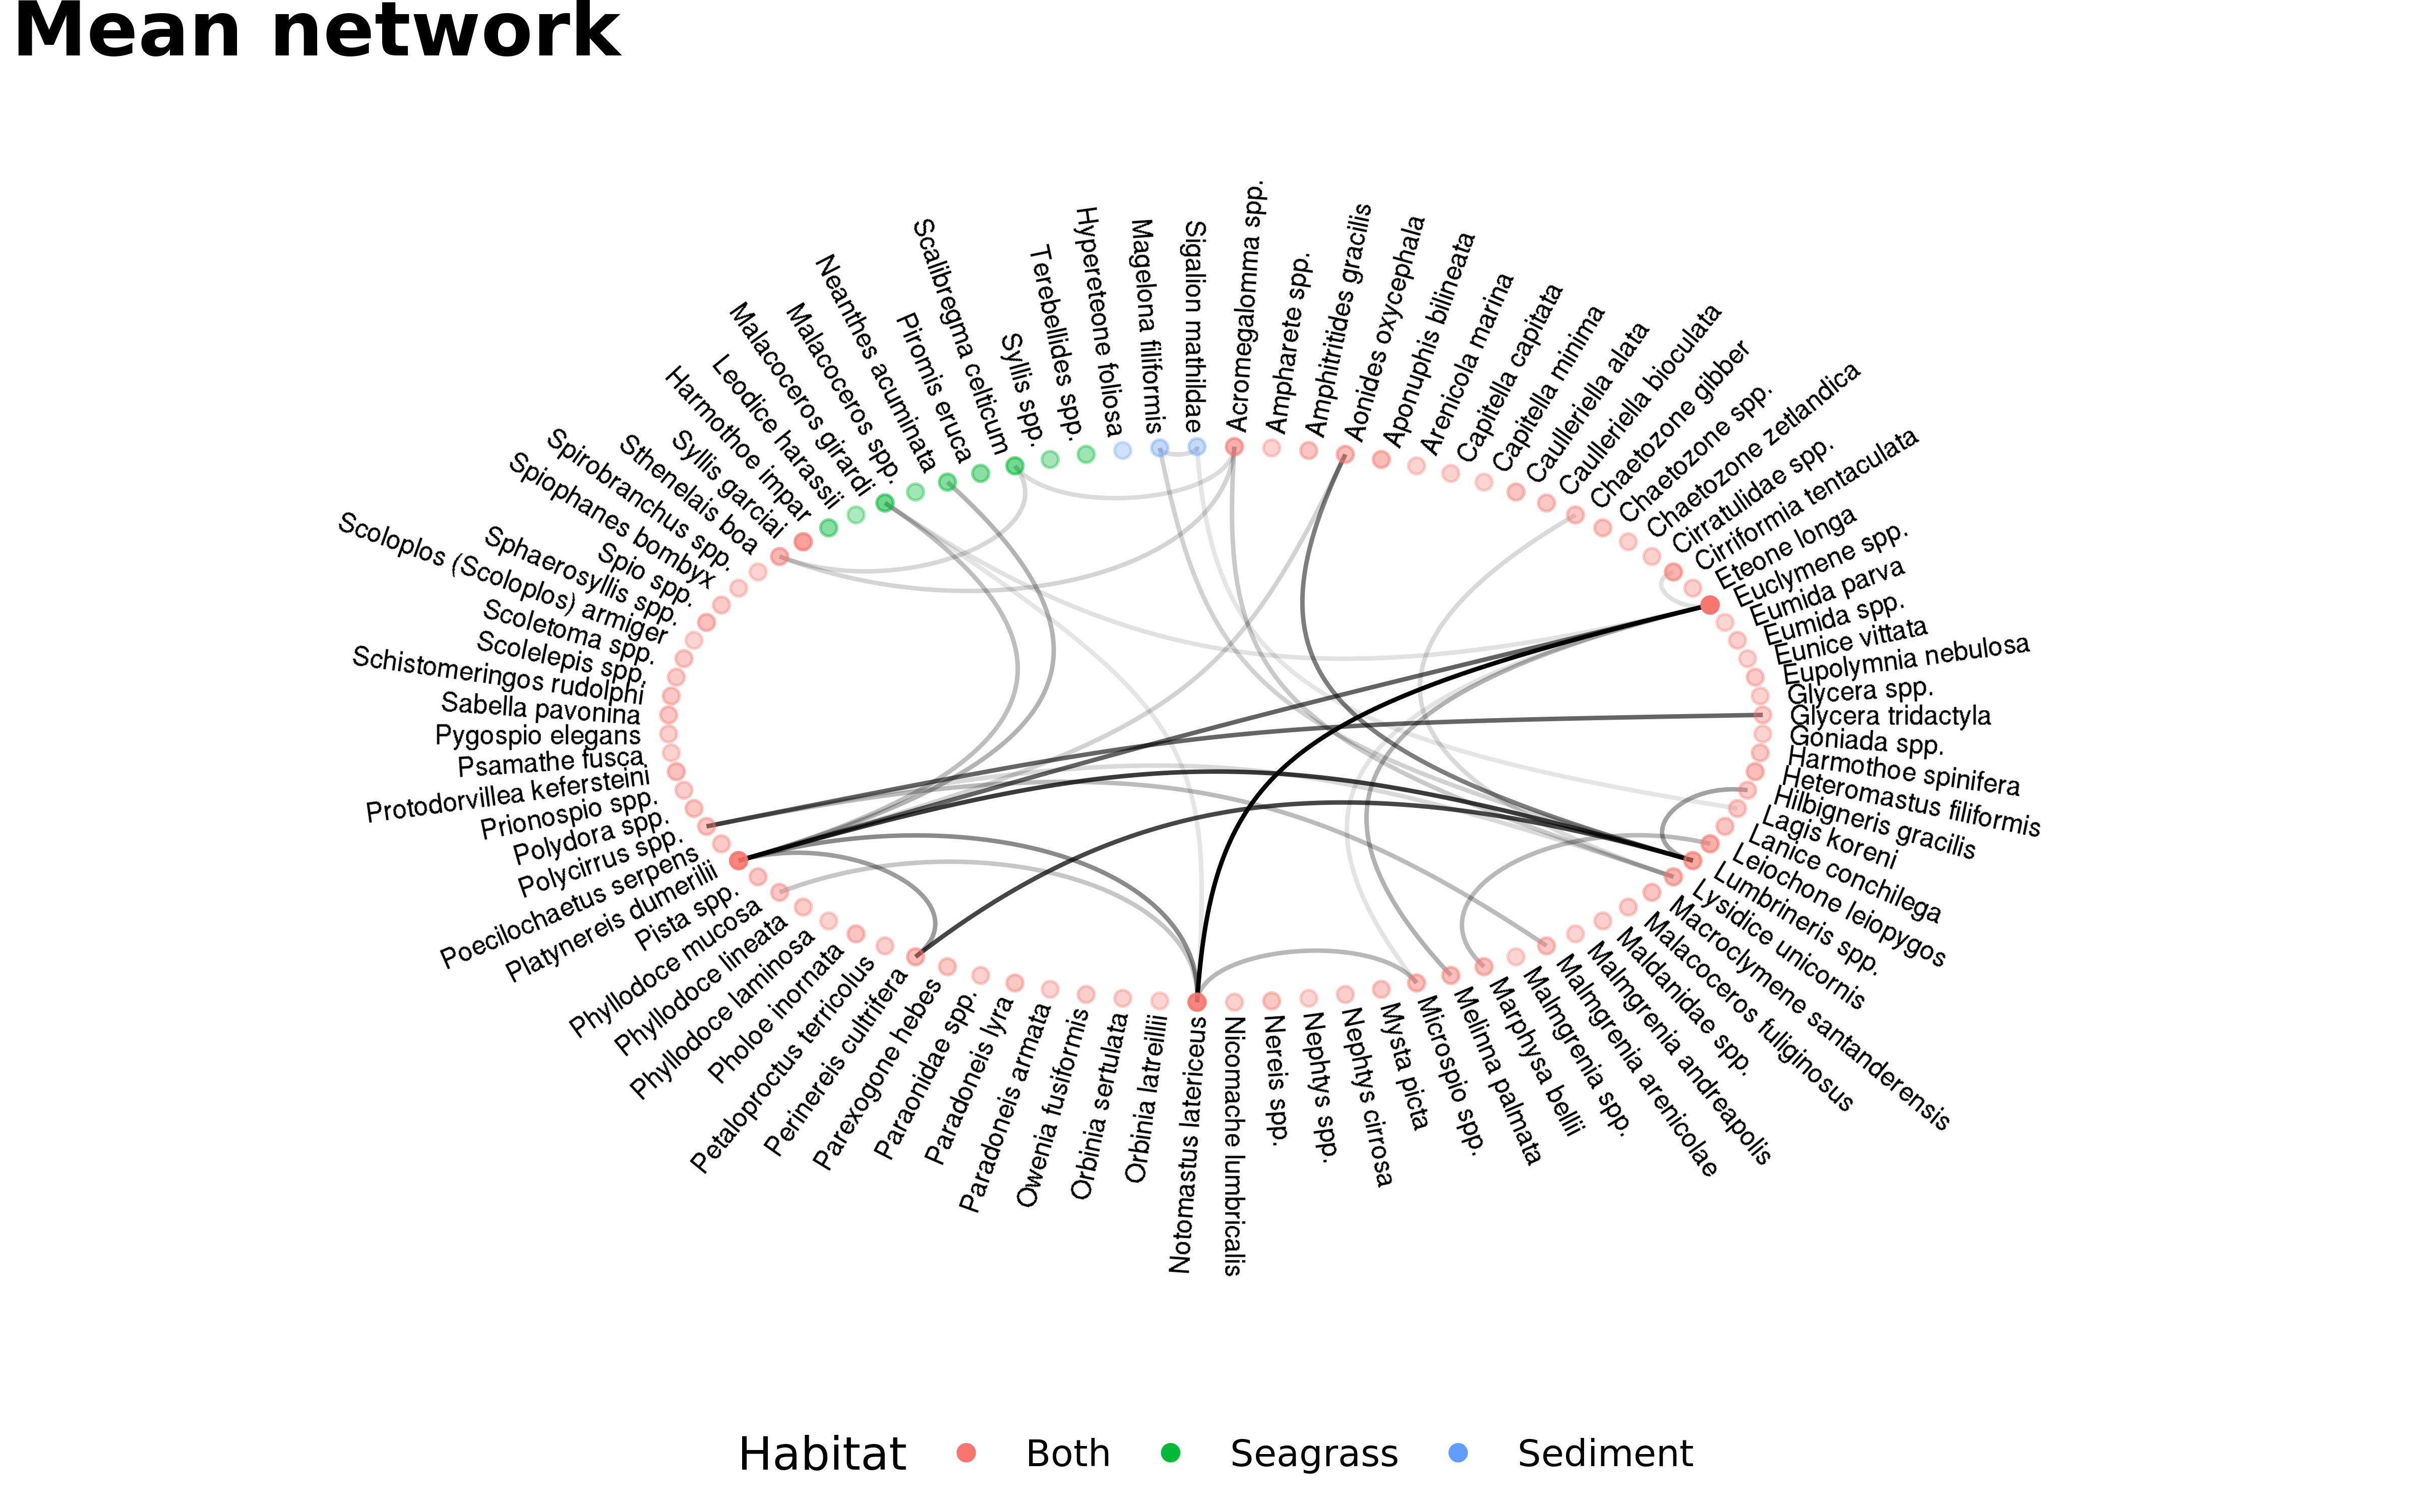
\includegraphics{figures/mean-network-1.png}
\caption{Réseau inféré moyen qui présente des probabilités d'interaction
moyennées sur l'ensemble des réseaux reconstruits décrits dans le
Tableau 2 . Les points rouges représentent les taxa de polychètes
retrouvés dans les deux habitats, les verts ceux retrouvés uniquement
dans les herbiers et les bleus ceux présents seulement dans les
sédiments meubles. Seules les arrêtes ayant une probabilité supérieure à
\(0,2\) sont affichées. L'opacité des arrêtes est proportionnelle à leur
importance dans le réseau (mesurée par la centralité de
Katz)}\label{fig:meannet}
}
\end{figure}

Plusieurs réseaux d'interactions peuvent être dérivés de \emph{HMSC},
une association résiduelle pouvant être extraite pour chacun des
facteurs aléatoires inclus dans le modèle. La Figure 6 présente par
exemple le réseau reconstruit sur la base des corrélations résiduelles
associées au facteur aléatoire temporel (années). Il est intéressant de
noter que seules des corrélations positives entre espèces sont présentes
dans ce réseau alors que les réseaux liés aux facteurs sites ou
habitats, ou que les réseaux issus des autres modèlent incluent aussi
des corrélations négatives (\cref{fig:nethmschiersite} et
\ref{fig:nethmschierhab} en annexe).

\begin{figure}
\hypertarget{fig:hmschierannee}{%
\centering
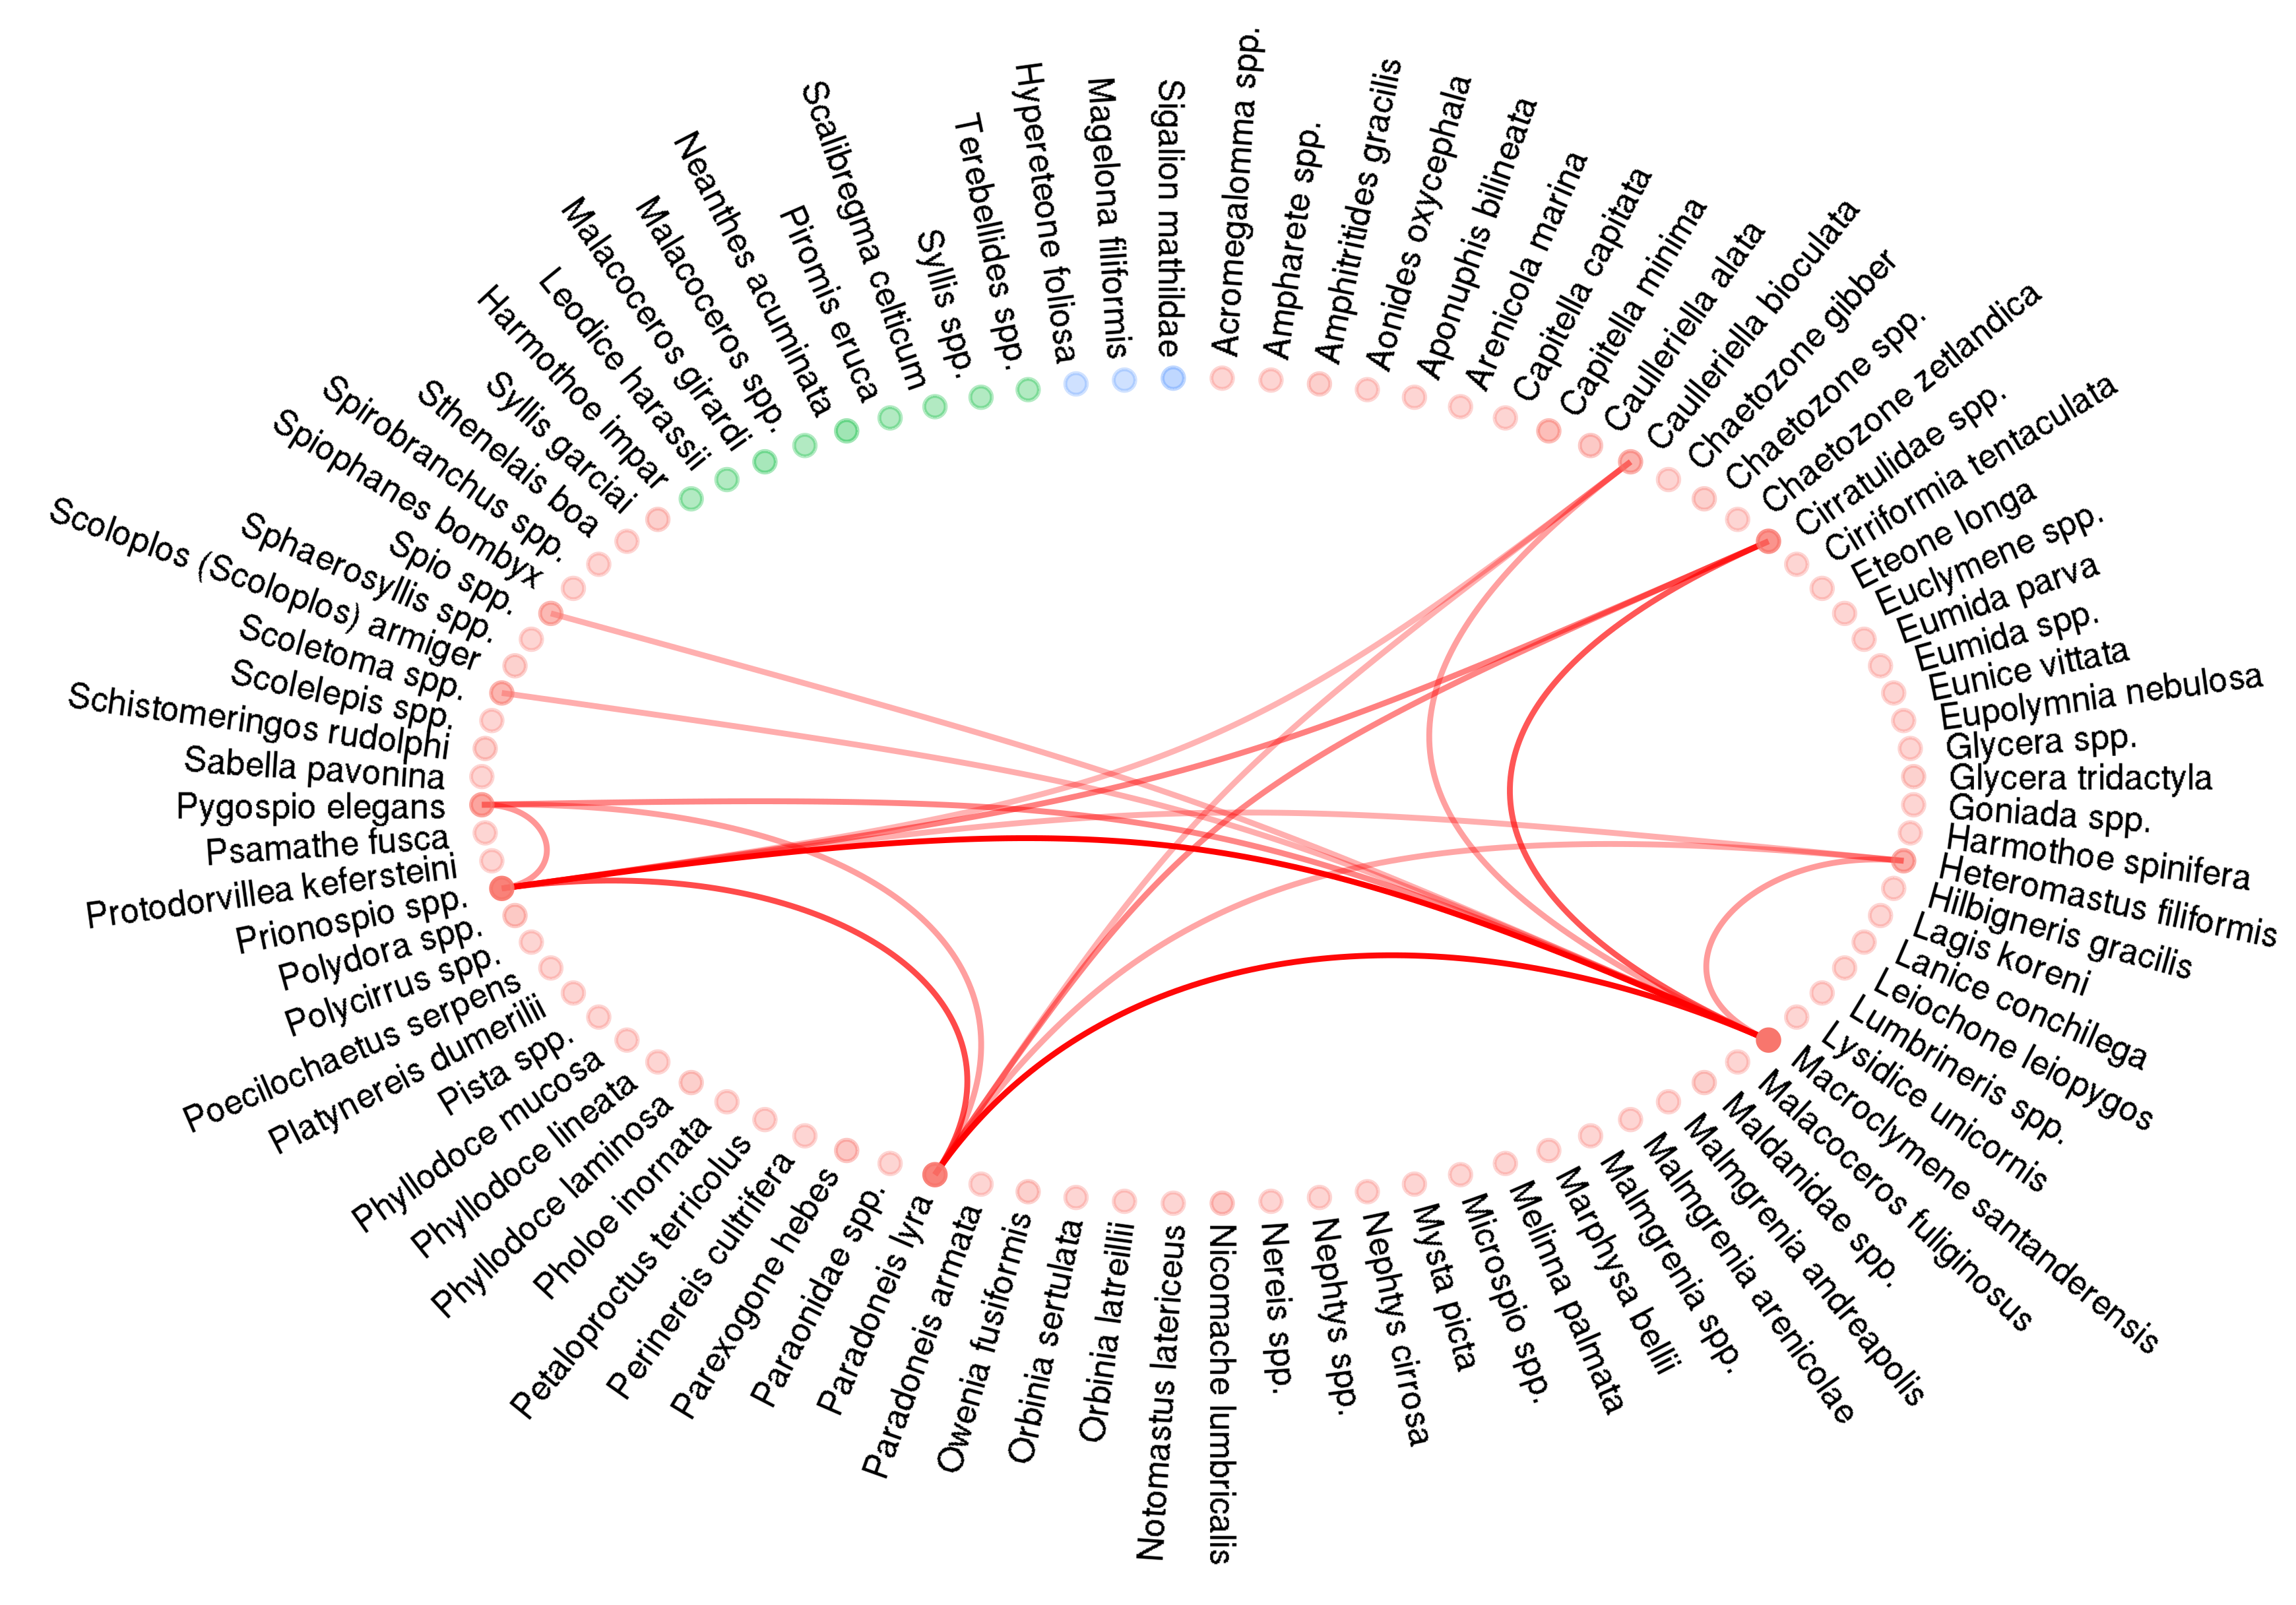
\includegraphics{figures/hmsc-hier-annee-network-1.png}
\caption{Réseau reconstruit avec EMTree sur la base des corrélations
résiduelles associées à l'effet aléatoire temporelle du modèle
\emph{HMSC\_hier}. Les points rouges représentent les taxa de polychètes
retrouvés dans les deux habitats, les verts retrouvés uniquement dans
les herbiers et les bleus dans les sédiments meubles. Seules les arrêtes
ayant une probabilité supérieure à \(0,2\) sont affichées. L'opacité des
arrêtes est proportionnelle à leur probabilité. L'opacité des points est
proportionnelle à leur importance dans le
réseau.}\label{fig:hmschierannee}
}
\end{figure}

\hypertarget{avis-des-experts-du-taxon-des-polychuxe8tes}{%
\subsubsection{Avis des experts du taxon des
polychètes}\label{avis-des-experts-du-taxon-des-polychuxe8tes}}

L'analyse de concordance de Kendall montre qu'il n'y a pas de consensus
significatif entre les différents experts quant à la probabilité
d'interaction entre les espèces qui leur ont été soumises (\(W + 0,26\),
\(p > 0,2\)). Résumer ces notes attribuées par les experts en deux
catégories seulement (interaction possible ou impossible), ne modifie
pas cet absence de consensus entre les experts (\(W = 0,2\),
\(p > 0,44\)). Cette absence de concordance entre experts rend difficile
la validation des interactions inférées par les modèles, mais il semble
que les probabilités d'interactions prédites ne correspondent pas à la
vision globale des experts (\cref{fig:expert}). En effet, les
interactions prédites sur l'ensemble des modèles comme étant les plus
probables sont plus souvent qualifiées d'impossible par les experts que
de potentiellement possible. Pour certaines interactions, il faut
cependant noter que l'avis des experts était unanime, et il a ainsi été
possible d'interpréter qualitativement le sens de certaines interactions
prédites via des discussions directes avec certains experts.

\begin{figure}
\hypertarget{fig:expert}{%
\centering
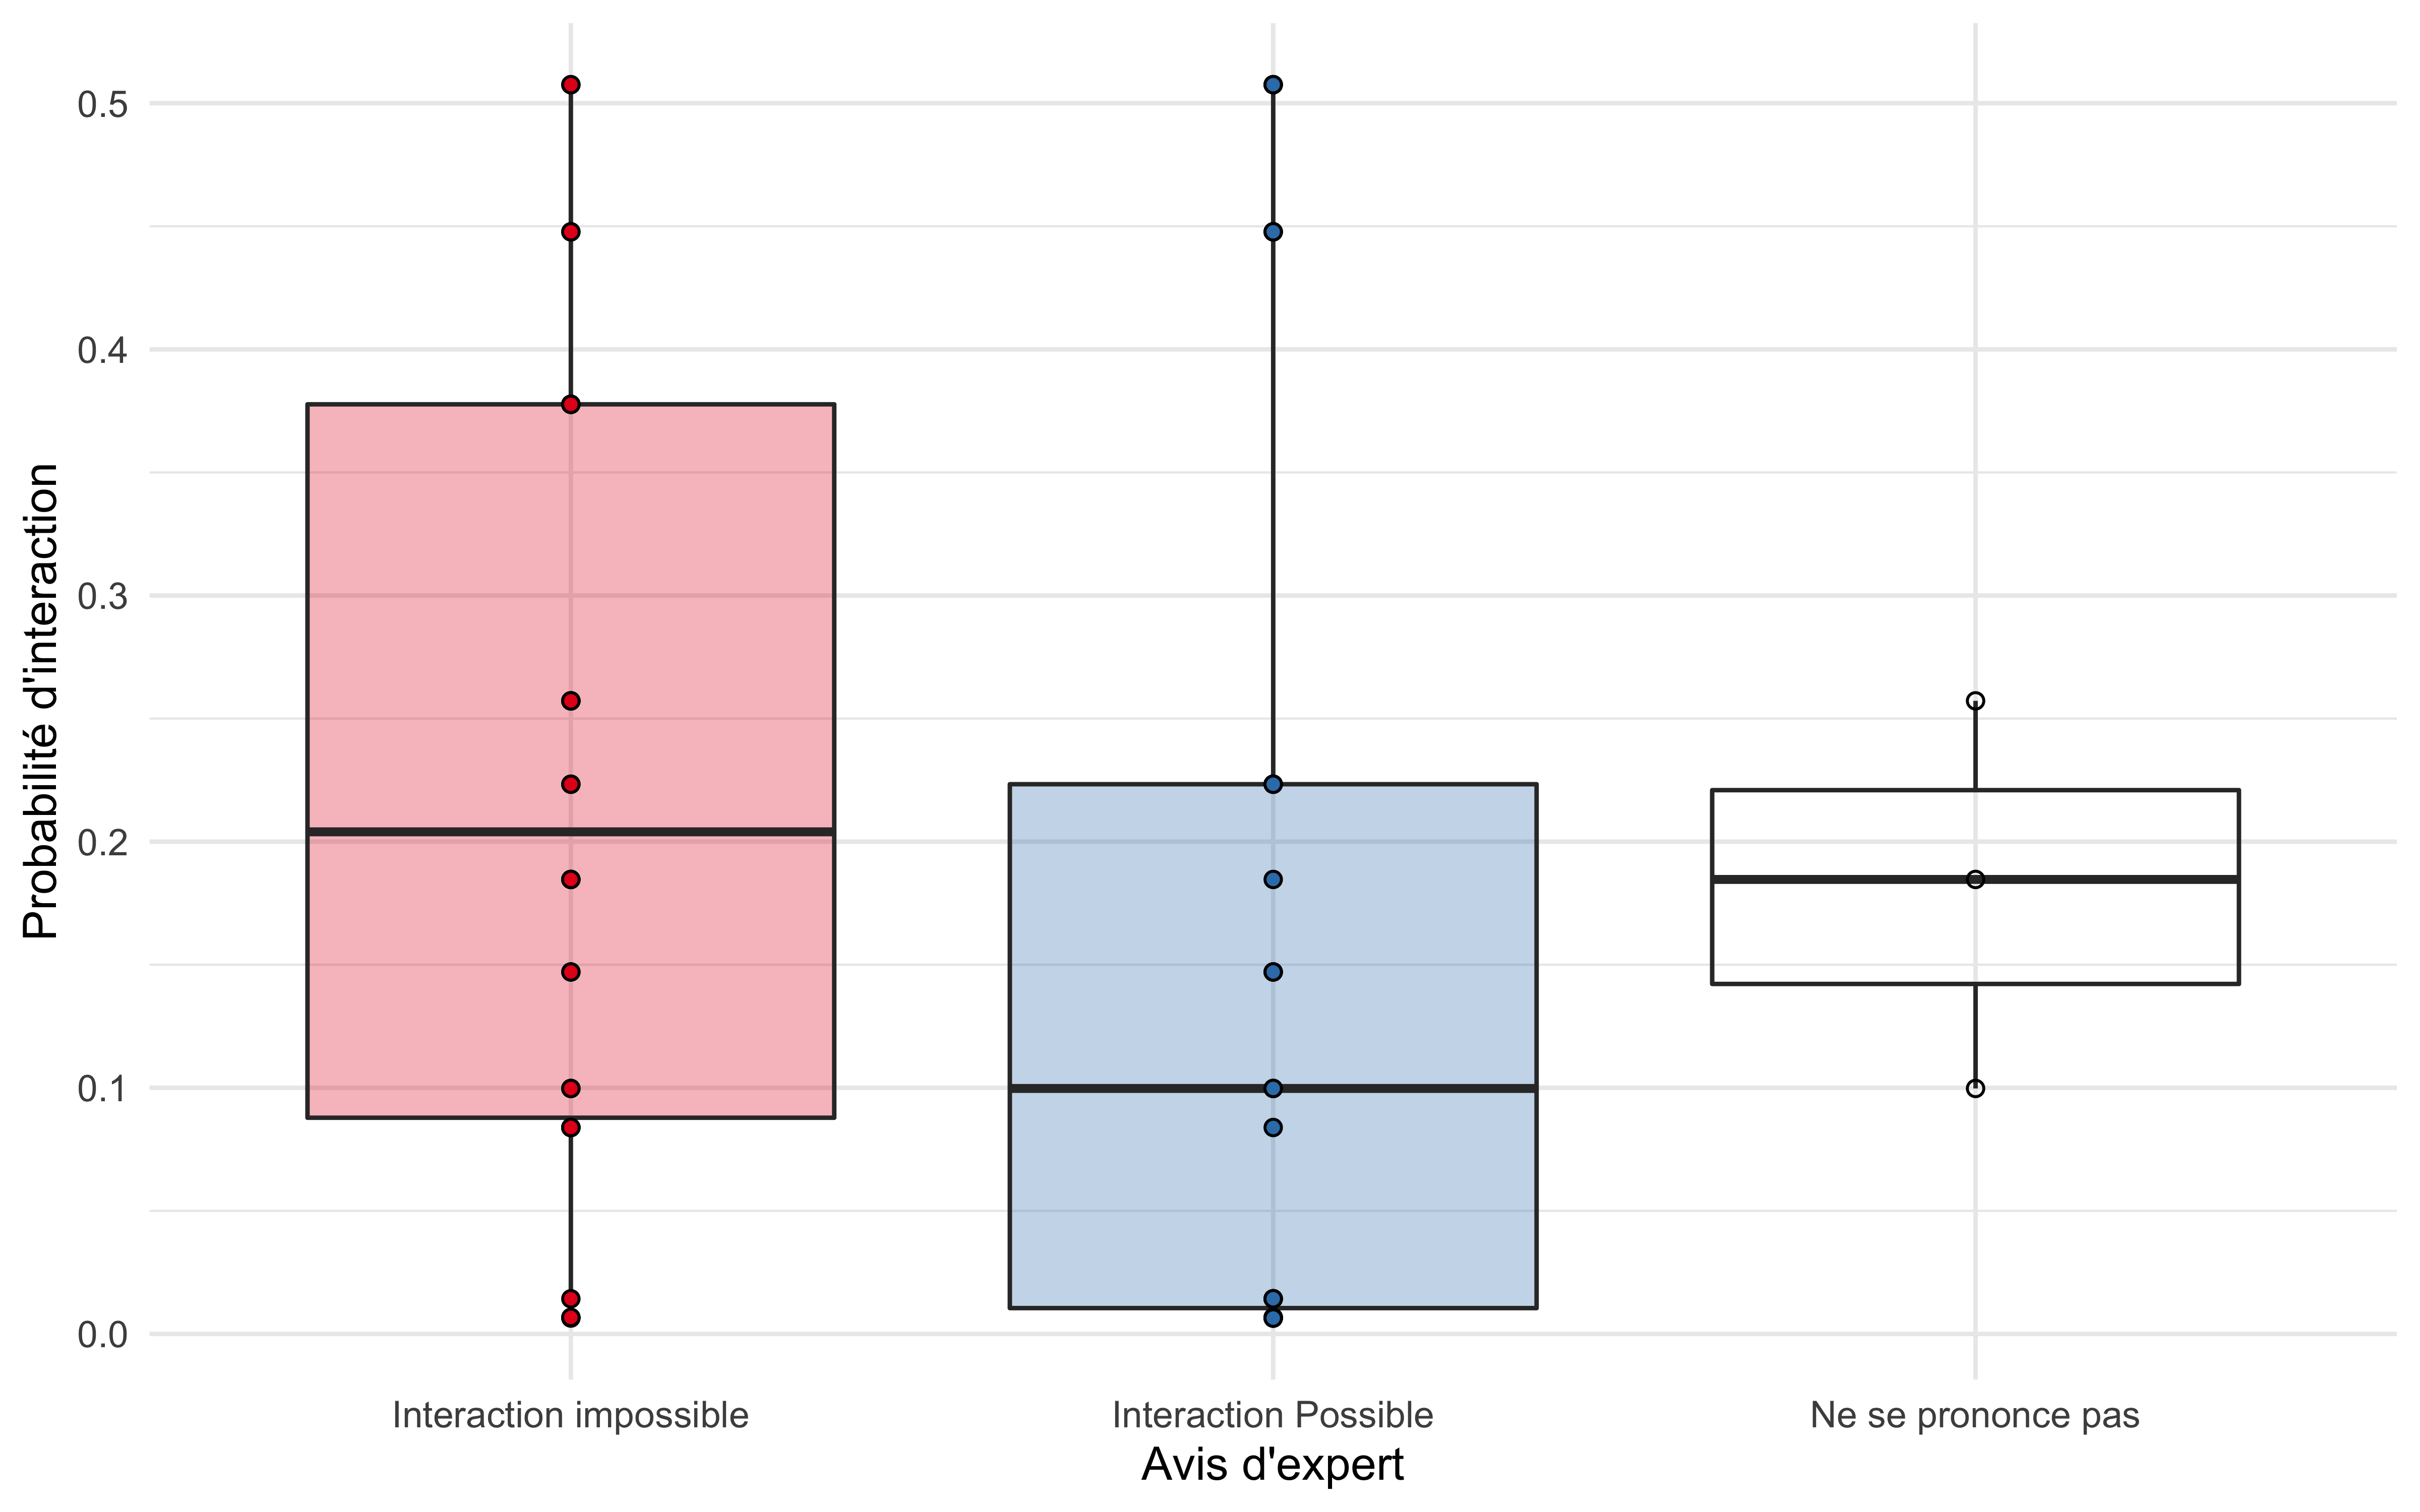
\includegraphics{figures/expert-option-2.png}
\caption{Avis des experts quant à la possibilité ou d'une interaction en
fonction des probabilités d'interaction moyenne prédite par les modèles.
La taille des points est proportionnelle au nombre d'experts ayant donné
la même réponse.}\label{fig:expert}
}
\end{figure}

\hypertarget{couxfbt-de-calcul}{%
\subsection{Coût de calcul}\label{couxfbt-de-calcul}}

Chaque modèle présente des caractéristiques propres en termes de coup de
calcul (\cref{tbl:coutcalc}). Les modèles implémentés sous \emph{HMSC}
présentent les temps de calcul les plus longs, mais leur coût en mémoire
vive reste cependant faible. Le temps de calcul augmente
considérablement avec le nombre d'effets aléatoires passant de plus de
25h pour le modèle le plus simple (sans effet aléatoire) à près de 458h
pour le modèle le plus complexe (trois effets aléatoires indépendants).
Comme attendu, \emph{GLLVM} se révèle être une implémentation
particulièrement rapide, étant même plus rapide à ajuster que le modèle
sans effet aléatoire \emph{HMSC\_reg}. Toutefois, sa vitesse est
largement contrebalancée par le coût important en mémoire vive. Ce
modèle a nécessité plus de 68 Go de RAM pour pouvoir être ajusté.
\emph{PLN} quant à lui est le modèle le plus économe à ajuster, il n'a
besoin que de trois minutes et moins de 500 Mo de RAM pour être ajusté.

{\small
\begin{longtable}[]{@{}lcc@{}}
\caption{Coût de calculs des différents modèles.
\label{tbl:coutcalc}}\tabularnewline
\toprule
Modèle & Temps de calcul (h : mn) & RAM (Go)\tabularnewline
\midrule
\endfirsthead
\toprule
Modèle & Temps de calcul (h : mn) & RAM (Go)\tabularnewline
\midrule
\endhead
\emph{HMSC\_reg} & \(25:27\) & \(0,49\)\tabularnewline
\emph{HMSC\_samp} & ~\(170:56\) & \(0,69\)\tabularnewline
\emph{HMSC\_hier} & \(457:50\) & \(0,73\)\tabularnewline
\emph{PLN} & ~\(00:03\) & ~\(0,37\)\tabularnewline
\emph{GLLVM} & ~\(13:43\) & \(68,1\)\tabularnewline
\bottomrule
\end{longtable}}\FloatBarrier


\hypertarget{discussion}{%
\section{Discussion}\label{discussion}}

\hypertarget{comprendre-et-pruxe9dire-la-diversituxe9-benthique}{%
\subsection{Comprendre et prédire la diversité
benthique}\label{comprendre-et-pruxe9dire-la-diversituxe9-benthique}}

Les différents modèles présentés ici n'expliquent que partiellement la
variabilité des assemblages de polychètes. Ainsi, sur les 92 espèces du
jeu données d'apprentissage, seules quelques espèces comme
\emph{Notomastus latericeus} (n°1), \emph{Euclymene spp.},
\emph{Lumbrineris spp.} (n°3), \emph{Nephtys cirrosa} (n°2) ou bien
\emph{Owenia fusiformis} (n°7) sont convenablement expliqués par les
modèles.\footnote{Les numéros correspondent aux entrées dans le
  \cref{tbl:sp} .}

Les modèles tels que \emph{HMSC\_hier} et \emph{HMSC\_samp} semblent
tirer parti de leur structure hiérarchique pour expliquer convenablement
un plus grand nombre d'espèces par rapport aux modèles ne disposant pas
d'une telle structure. En effet, ce sont principalement les effets
aléatoires qui expliquent le plus de la variation des espèces. Ainsi, le
manque de pouvoir explicatif des variables environnementales semble
montrer que la niche écologique des espèces de cette communauté est mal
définie dans nos modèles. Les variables environnementales sélectionnées
ne sont probablement pas mesurées à la bonne échelle, ou leur effet ne
peut être distingué correctement des effets spatiaux. Ce manque de
pouvoir explicatif des variables environnementales limite la
transférabilité de ces modèles à d'autres lieux et environnements.

Nos modèles prédisent relativement bien l'occurrence des espèces et donc
la richesse des assemblages et leurs variations dans l'espace et le
temps. Ces résultats sont consistants avec les précédentes comparaisons
qui ont été faites de ces modèles (Norberg \emph{et al.}
\protect\hyperlink{ref-Norberg_2020}{2019}; Momal \emph{et al.}
\protect\hyperlink{ref-Momal_2020}{2020}). Notamment, la richesse des
assemblages est apparue particulièrement bien prédite lorsque des seuils
espèce-spécifique ont été utilisés pour convertir l'abondance en
présence/absence (Ashcroft \emph{et al.}
\protect\hyperlink{ref-Ashcroft_2017}{2017}). L'utilisation de cette
approche par seuil, largement inspirée des approches de cartographie à
partir de \emph{SDM} (Lawson \emph{et al.}
\protect\hyperlink{ref-Lawson_2013}{2013}), est inédite à notre
connaissance pour l'analyse des prédictions issues de \emph{JSDM}. Une
comparaison des performances de cette approche (modélisation de
l'abondance puis seuils pour convertir en occurrence) avec de modèles
entrainés directement sur des données d'occurrence (ce qui était fait
jusqu'à présent, e.g~; Norberg \emph{et al.}
(\protect\hyperlink{ref-Norberg_2020}{2019})) pourrait permettre
d'évaluer plus clairement la validité de l'approche. Cependant, il nous
semble potentiellement plus prometteur de prendre en compte
l'information contenue dans l'abondance des espèces pour entrainer les
modèles puis d'utiliser des seuils appropriés pour modéliser la richesse
des communautés, que d'utiliser une transformation brute des abondances
en présence/absence, ou encore que de négliger complètement
l'information contenue dans l'abondance des espèces. Cependant, si l'une
des promesses des \emph{JSDM} est bien de pouvoir prédire également
l'abondance des espèces, la performance des modèles testés ici est
apparue décevante. Le \emph{RMSE} maximal pour le meilleur modèle,
\emph{HMSC\_reg}, est ainsi de l'ordre de \(10^4\), ce qui justifie
d'autant plus l'utilisation des seuils espèce-spécifique pour prédire la
richesse des communautés à partir de \emph{JSDM} entrainé sur des
données d'abondances.

Sur ce critère d'abondance, \emph{GLLVM} est le moins performant des
modèles testés. Cela peut s'expliquer par plusieurs facteurs. Notamment,
la distribution négative binomiale a été utilisée pour le modèle
\emph{GLLVM} contrairement aux autres modèles qui utilisent la
distribution de Poisson lognormal. Dans le cadre plus classique de
\emph{SDM}, cette distribution négative binomiale montre en général de
plus faibles capacités à modéliser l'abondance des espèces que d'autres
distributions (Potts \& Elith \protect\hyperlink{ref-Potts_2006}{2006}).
Ce manque de performance prédictif a également été montré face à la
distribution de Poisson lognormal (Trinh \emph{et al.}
\protect\hyperlink{ref-Trinh_2013}{2013}). Il semblerait que la
structure de la variance de la distribution négative binomiale permette
trop de surdispersion par rapport à d'autres distributions, et donc
donne des prédictions moins bonnes. De plus, l'utilisation d'effets
aléatoires au niveau de l'observation comme le permet la distribution de
Poissoin lognormale permet de mieux prendre en compte la surdispersion
des données d'abondances en permettant plus de souplesse au modèle
(Harrison \protect\hyperlink{ref-Harrison_2014}{2014}). Enfin, il
semblerait que l'utilisation dans \emph{GLLVM} d'approximation
variationnelle pour améliorer les vitesses de calcul, puisse affecter la
précision des résultats par rapport aux autres approches (Warton
\emph{et al.} \protect\hyperlink{ref-warton2015}{2015}). Dans
l'ensemble, la faible qualité de la prédiction de l'abondance peut en
partie être expliquée par le faible pouvoir explicatif des variables
environnementales utilisées pour entrainer nos modèles. En ayant une
meilleure connaissance ou une meilleure prise en compte de la niche
écologique de ces espèces de polychètes, il serait possible d'améliorer
significativement la qualité prédictive de ces modèles (Leach \emph{et
al.} \protect\hyperlink{ref-Leach_2016}{2016}; Barbaro \emph{et al.}
\protect\hyperlink{ref-Barbaro_2019}{2019}). Dans le cadre de cette
étude, le nombre de variables environnementales prises en compte dans
les modèles a avant tout été limité pour des questions de coûts de
calculs et de nombre de paramètres à estimer. En prenant en compte
toutes les données existantes du suivi REBENT, il serait possible
d'utiliser plus de variables environnementales ainsi que des polynômes
de degrés plus élevés pour modéliser des relations non linéaires des
espèces avec leur environnement. Si cela était initialement envisagé,
les temps de calcul des modèles se sont révélés prohibitifs pour ce
genre d'approches, et le choix a été fait de se limiter aux variables
potentiellement les plus intéressantes sur la base de travaux précédents
(Boyé \protect\hyperlink{ref-Boye_2019b}{2019}).

\hypertarget{ruxf4le-et-infuxe9rence-des-interactions-biotiques}{%
\subsection{Rôle et inférence des interactions
biotiques}\label{ruxf4le-et-infuxe9rence-des-interactions-biotiques}}

Prendre en compte les interactions dans nos modèles améliore globalement
leurs capacités de prédictions si nous les comparons aux résultats d'un
modèle sans effet aléatoire tel que \emph{HMSC\_reg}, qui se retrouve
toujours parmi les moins bons modèles. Ce résultat est en accord avec la
littérature, puisque la prise en compte des interactions biotiques
améliore les capacités prédictives des modèles linéaires (Wisz \emph{et
al.} \protect\hyperlink{ref-Wisz_2012}{2012}; Gavish \emph{et al.}
\protect\hyperlink{ref-Gavish_2017}{2017}; Staniczenko \emph{et al.}
\protect\hyperlink{ref-Staniczenko_2017}{2017}). Bien que la prise en
compte des interactions par les différents modèles se fait de la même
manière à l'aide de variables latentes, l'implémentation de ces
variables latentes change entre les modèles. Cette différence dans la
façon d'inclure ces interactions se répercute sur le rôle estimé des
facteurs environnementaux dans les modèles. L'indice de Trask a une
influence positive pour beaucoup d'espèces selon la plupert des modèles,
mais explique une faible variance. Cependant, en prenant en compte un
plus grand nombre de facteurs aléatoires, le modèle \emph{HMSC\_hier} a
démontré que son effet était largement inversé (et majoritairement
négatif). Cela semble suggérer que l'indice de Trask est une variable
fortement liée au site.

Malgré le fait que l'avis de nos experts ne concorde pas quant à la
probabilité des liens, certains liens du réseau moyen ont été identifiés
par les experts comme pouvant correspondre à des~interactions
proies-prédateurs. Par exemple, celles entre \emph{Perinereis
cultrifera} (n°12) et \emph{Lumbrineris spp.} (n°3), \emph{Magelona
filiformis} (n°9) et \emph{Sigalion mathildae} (n°22) ou bien encore
\emph{Scalibregma celticum} (n°27) et \emph{Sthenelais boa} (n°40). Par
ailleurs, la probabilité forte d'interaction entre \emph{Platynereis
dumerilii} (n°10) et \emph{Euclymene spp.} (n°5) et encore
\emph{Notomastus latericeus} (n°1) pourrait selon les experts traduire
de la compétition trophique et spatiale. En effet, \emph{Platynereis
dumerilii} (n°10) est un broutteur de microphytobenthos et les deux
autres espèces sont des déposivores (Jumars \emph{et al.}
\protect\hyperlink{ref-Jumars_2015}{2015}). Ces trois taxa vont donc
acquérir leur nourriture au même endroit, sur ou près de la surface du
sédiment. De plus, ces trois taxa sont également ceux avec la plus
grande centralité dans le réseau moyen. Cette importance dans le réseau
est peut-être liée à la forte dominance des espèces déposivores ou
broutteuses dans les habitats suivis (Boyé \emph{et al.}
\protect\hyperlink{ref-Boye_2019a}{2019}).

La structure de ces réseaux reconstruits assez particulière : la valeur
de la connectance est dix fois plus petite que celle observée pour
d'autres réseaux benthiques (Martinez
\protect\hyperlink{ref-Martinez_1992}{1992}; Dunne \emph{et al.}
\protect\hyperlink{ref-Dunne_2004}{2004}). Les réseaux reconstruits
présentent également une imbrication très faible par rapport à ce que
montre la littérature des réseaux trophiques benthique (Nordström
\emph{et al.} \protect\hyperlink{ref-Nordstrom_2015}{2015}). Ces
résultats, ainsi que le faible nombre d'interactions ayant une
probabilité supérieure à 0,2 est probablement lié à la nature des
communautés étudiées, et en particulier au focus de ce travail sur les
polychètes. En effet, des analyses de traits biologiques de ces
assemblages de polychètes ont suggéré précédemment une prédominance de
filtres biotiques et de processus neutres, et un faible rôle des
interactions biotiques, dans la structure de ces assemblages de
polychètes (Boyé \emph{et al.}
\protect\hyperlink{ref-Boye_2019a}{2019}). Les résultats de cette étude,
et notamment les faibles connectances observées sur l'ensemble des
modèles, semblent confirmer ces hypothèses. Cela peut aussi s'expliquer
par le fait que les polychètes ne forment pas un réseau à part entière
et que de nombreuses interactions avec d'autres phylums ne sont ainsi
pas représentées. En effet, il nous manque beaucoup d'acteurs pour
obtenir un réseau d'interaction d'une communauté benthique complète,
certains poissons et d'autres invertébrés par exemple, sont des
prédateurs de polychètes (Jankowska \emph{et al.}
\protect\hyperlink{ref-Jankowska_2019}{2019}), et ne sont pas inclus
dans les réseaux que nous avons reconstruits, alors que certains
bivalves peuvent avoir un rôle facilitateur important (Gagnon \emph{et
al.} \protect\hyperlink{ref-Gagnon_2020}{2020}), qui ne sont pas non
plus pris en compte.

Le nombre de liens identiques à travers tous les réseaux reconstruits
peut sembler étrange au premier regard. C'est une conséquence de la
manière dont sont générés ces graphes à l'aide de l'algorithme
\emph{EMtree} et de la façon dont sont calculés les liens dans le cadre
des réseaux écologiques probabilistes (Poisot \emph{et al.}
\protect\hyperlink{ref-Poisot_2015}{2015}). Pour reconstruire ces
réseaux \emph{EMtree} parcourt l'ensemble des arbres couvrants
possibles. Dans notre cas, notre communauté pour le jeu de donnée
d'apprentissage compte \(p = 92\) espèces, et il y a \(p^{p-2}\) arbres
couvrant possible différent, soit un total de \(5,51\times 10^{176}\).
Pour rappel, dans un cadre de réseaux probabilistiques, le nombre de
liens est calculé comme étant la somme des probabilités contenue dans la
matrice . \emph{EMtree} parcourant toujours le même espace d'arbre
couvrant possible. C'est pourquoi la somme des probabilités de la
matrice d'interaction (nombre de liens) est toujours identique, quelle
que soit la méthode, mais qu'il est possible d'avoir de la variabilité
dans le nombre de liens et la connectance, car chaque lien n'a pas la
même probabilité en fonction du réseau.

Le manque de concordance entre nos différents experts quant à la
probabilité des interactions reconstruites s'explique de différente
façon. Tout d'abord, les polychètes sont des animaux qui restent assez
mal connus actuellement (Troudet \emph{et al.}
\protect\hyperlink{ref-Troudet_2017}{2017}). Il reste de nombreuses
interrogations quant à leurs modes de vie et les possibles interactions
qu'il existe au sein de ce clade (Jumars \emph{et al.}
\protect\hyperlink{ref-Jumars_2015}{2015}; Boyé \emph{et al.}
\protect\hyperlink{ref-Boye_2019a}{2019}). De plus, certains patrons de
co-occurrence ont semblé étranges à nos experts. Le très fort nombre de
corrélations positives obtenues par l'effet aléatoire temporelle du
modèle \emph{HMS\_hier} n'était pas attendu (\cref{fig:hmschierannee}).
En effet, l'hypothèse initiale était que les associations résiduelles
dans le temps seraient plus à même de représenter des interactions
biotiques que des effets résiduels liés à la variabilité spatiale ou à
l'habitat associés à des variables abiotiques non considérées dans les
modèles. Dans cette hypothèse, des interactions de type proie prédation
ou compétition se serait alors traduite par des associations négatives
dans le temps. Le fait que seules des interactions positives soient
retrouvées pourrait s'expliquer par différents facteurs non exclusifs
tels que (1) une prépondérance d'effets facilitateur dans ces
communautés benthiques intertidales (Bertness \& Leonard
\protect\hyperlink{ref-Bertness_1997}{1997}; Gribben \emph{et al.}
\protect\hyperlink{ref-Gribben_2019}{2019}) (2) l'échelle
spatio-temporelle du suivi REBENT~: à larges échelles, des prédateurs
auront tendance à être là où leurs proies se trouvent, résultant en des
associations positives, là où des dynamiques temporelles à plus fines
échelles montrerais des associations négatives (e.g.~modèle de
Lokta-Volterra). Enfin, Thurman \emph{et al.}
(\protect\hyperlink{ref-Thurman_2019}{2019}) en utilisant des données
empiriques ont montré que plus une espèce interagissait avec d'autres,
plus la corrélation résiduelle entre ces espèces dans un \emph{JSDM}
était faible et tendaient à être positif. Etant donnée la grande
diversité de notre jeu de données, cela pourrait expliquer à la fois les
faibles probabilités d'interactions et le grand nombre d'interactions
positives observées.

Enfin, malgré les limitations soulevées précédemment, il est important
de noter que notre méthodologie de reconstructions des réseaux
d'interactions nous permet d'éviter plusieurs des écueils résumés par
(Blanchet \emph{et al.} \protect\hyperlink{ref-Blanchet_2020}{2020})
quant à l'utilisation faite classiquement des \emph{JSDM} pour inférer
des interactions entre espèces. Tout d'abord, notre travail utilise des
données d'abondance qui sont plus riche en informations que les données
de présence/absence. De plus, nous utilisons une méthode basée sur les
graphes pour reconstruire les interactions, ce qui évite que les
interactions indirectes soient confondues avec des interactions
directes(Chiquet \emph{et al.}
\protect\hyperlink{ref-Chiquet_2019}{2019}; Momal \emph{et al.}
\protect\hyperlink{ref-Momal_2020}{2020}), renforçant ainsi la
vraisemblance écologique des interactions inférées avec des probabilités
fortes.

\hypertarget{forces-et-faiblesses-des-diffuxe9rentes-approches}{%
\subsection{Forces et faiblesses des différentes
approches}\label{forces-et-faiblesses-des-diffuxe9rentes-approches}}

Dans leur ensemble, les modèles testés dans ce travail sont assez
prometteurs. Leur capacité à prédire convenablement l'occurrence des
espèces et leurs dynamiques spatiales et temporelles pourrait servir à
évaluer l'impact de certains changements environnementaux sur la
composition et la richesse des communautés. Cependant, l'importance des
effets aléatoires dans la capacité prédictive de ces modèles pourrait
limiter leur transférabilité (Yates \emph{et al.}
\protect\hyperlink{ref-Yates_2018}{2018}) à d'autres zones géographiques
ou à d'autres habitats. En revanche, la capacité de modèles comme
\emph{HMSC}, grâce à leur structure hiérarchique, à découper les
corrélations résiduelles entre espèces selon différents facteurs
aléatoires offre la possibilité d'obtenir une vision plus fine sur les
possibles interactions et associations interspécifiques dans l'espace et
le temps.

Bien que certains modèles semblent sensiblement plus performants que
d'autres, aucun n'est parfait : ``Tous les modèles sont faux, mais
certains sont utiles.'' (Box \protect\hyperlink{ref-Box_1979}{1979}).
Ainsi, chaque modèle représente un trade-off entre une plus grande
précision des paramètres estimés et un coût de calcul plus élevé.
\emph{HMSC\_hier} est le modèle le plus précis et le plus performant en
termes prédictifs dans notre étude, mais cela au prix d'un temps de
calcul extrêmement élevé (i.e.~des centaines d'heures de calculs sur le
supercalculateur DATARMOR). Ainsi, si la question de recherche se trouve
être la prédiction de l'occurrence, il est préférable de se tourner vers
\emph{GLLVM}, notamment si les délais de la recherche sont réduits et si
la mémoire vive nécessaire est disponible, car sa capacité à prédire la
richesse des assemblages reste satisfaisante par rapport à \emph{HMSC}.
Si l'on ne dispose pas assez de mémoire vive, une alternative
représentant un bon compromis pourrait être \emph{PLN}, bien que la
simplicité de ce modèle (une seule distribution possible) puisse lui
faire manquer de polyvalence (par exemple sur des données de
présence/absence ou de biomasses qui nécessiterait d'autres
distributions, Niku \emph{et al.}
(\protect\hyperlink{ref-Niku_2019}{2019}\protect\hyperlink{ref-Niku_2019}{b})).

Pour ce qui est d'inférer les interactions entre espèces à partir des
données d'observations grâce à ces modèles joints, Blanchet \emph{et
al.} (\protect\hyperlink{ref-Blanchet_2020}{2020}) mettent en avant
plusieurs limites, tant d'un point de vue théorique que pratiques, qu'il
semble important de rappeler ici. Un signal de co-occurrence peut par
exemple, provenir de variables environnementales mal prises en compte
par le modèle. Bien que les variables latentes puissent capturer ce
signal, il n'est pas possible d'en différencier le signal biotique du
signal d'une ou plusieurs variables environnementales manquantes
(Blanchet \emph{et al.} \protect\hyperlink{ref-Blanchet_2020}{2020}).
Lorsque le signal de corrélation entre taxa est faible, le nombre
d'échantillons nécessaire pour détecter une interaction est extrêmement
élevé. L'ordre de grandeur du nombre d'échantillons nécessaire peut
dépasser de l'ordre du millier, ce qui n'est pas atteint dans ce
travail. Enfin, les modèles de JSDM sont incapables de prédire les
interactions négatives très fortes (e.g.~cas de l'exclusion
compétitive), car ces dernières sont incompatibles avec la coexistence
(Blanchet \emph{et al.} \protect\hyperlink{ref-Blanchet_2020}{2020}).
Ainsi, ces méthodes ne pourront surement pas dans un avenir proche, et
en l'état, permettre d'inférer de manière réaliste des réseaux
écologiques. Elles peuvent en revanche orienter les recherches vers des
interactions probables et apporter des informations utiles pour mettre
en perspectives des études réalisées à plus fines échelles, comme le
montrent les retours des experts dans cette étude. Pour cela, il est
important d'éviter les principaux écueils soulevés par Blanchet \emph{et
al.} (\protect\hyperlink{ref-Blanchet_2020}{2020}), ce que visait la
méthodologie employée dans cette étude, notamment par l'utilisation
d'\emph{EMtree} et de données d'abondances.

\hypertarget{perspectives}{%
\subsection{Perspectives}\label{perspectives}}

Certains des modèles utilisés dans ce travail présentent la propriété
d'être assez flexible. \emph{HMSC} et \emph{GLLVM} peuvent en effet
inclure des traits fonctionnels ou la phylogénie pour améliorer un peu
plus les prédictions, notamment pour les espèces rares. En effet, pour
modéliser des taxa les plus rares \emph{HMSC} ``emprunte'' de
l'information aux taxa les plus communs grâce aux traits et à la
phylogénie. Ce type de modèle fait l'hypothèse que deux espèces aux
traits similaires ou proche sur le plan phylogénétique réagissent de
façon analogue aux gradients environnementaux (Ovaskainen \& Abrego
\protect\hyperlink{ref-Ovaskainen_2020}{2020}). En plus d'améliorer les
résultats, l'inclusion des traits ou de la phylogénie pourrait fournir
une aide à l'interprétation des résultats grâce à une perspective un peu
plus mécaniste. Une autre voie d'amélioration possible pour \emph{HMSC}
serait d'implémenter de façon explicite des effets aléatoires spatiaux
et temporels en prenant en compte des notions de distances (Ovaskainen
\emph{et al.}
\protect\hyperlink{ref-Ovaskainen_2017a}{2017}\protect\hyperlink{ref-Ovaskainen_2017a}{b}).

Ces modèles pourraient également bénéficier d'un autre axe de validation
se basant cette fois-ci sur la diversité. Une suite logique aux analyses
spatiotemporelles mises en place dans ce travail de recherche serait les
analyses de trajectoires des communautés telles que décrites par de
Cáceres \emph{et al.} (\protect\hyperlink{ref-De_Caceres_2019}{2019}).
L'utilisation des métriques proposées par de Cáceres \emph{et al.}
(\protect\hyperlink{ref-De_Caceres_2019}{2019}) permettraient de
comparer les trajectoires des communautés prédites avec les trajectoires
observées. Il serait ainsi possible de voir si certains des \emph{JDSM}
modélisent adéquatement la dynamique temporelle des communautés en
termes de composition et non plus seulement en termes de richesse comme
dans cette étude.

Pour ce qui est des perspectives sur l'inférence des réseaux
d'interactions, il convient de noter que les réseaux d'interactions en
écologie présentent des caractéristiques particulières (Pascual \&
Jennifer \protect\hyperlink{ref-Pascual_2006}{2006}) . C'est pourquoi il
serait intéressant de tester les capacités de reconstruction des réseaux
d'interactions de ces \emph{JDSM} via des simulations, sur des réseaux
aux propriétés connus basés sur des données d'abondances générées in
silico. Cela permettrait de mieux comprendre si certaines propriétés
particulières comme la faible imbrication des réseaux d'interaction
observée est un artefact numérique ou bien une réelle propriété du
réseau lié aux assemblages de polychètes étudiés ici. Les interactions
inférées quant à elles pourraient profiter d'autres moyens de validation
en plus des dires d'experts comme des méthodes issues de l'écologie
trophique et notamment expérimentales (isotopes, contenus stomacaux~;
Majdi \emph{et al.} (\protect\hyperlink{ref-Majdi_2018}{2018})).
Toutefois, le manque de connaissance expérimentale sur ces taxa peut
représenter le frein le plus important à la mise en place de cette forme
de validation.

Enfin, si ce travail de par son focus réduit aux communautés de
polychètes illustre bien la problématique commune en écologie marine du
manque de données fiables sur tous les taxons à l'échelle de tout un
écosystème, les méthodes testées ici peuvent possiblement trouver des
applications à des jeux de données plus exhaustifs grâce aux dernières
méthodes de métabarcoding (Djurhuus \emph{et al.}
\protect\hyperlink{ref-Djurhuus_2020}{2020}). Allier les \emph{JSDM} à
ces méthodes omiques permettrait d'obtenir une meilleure vision
d'ensemble de la biodiversité et donc des réseaux d'interaction
écologiques. Pour cela, l'un des principaux défis auxquels feront face
les \emph{JSDM} concernera l'optimisation de leur coût de calcul.

\hypertarget{bibliographie}{%
\section{Bibliographie}\label{bibliographie}}

\hypertarget{refs}{}
\begin{cslreferences}
\leavevmode\hypertarget{ref-Araujo_2019}{}%
Araújo, M.B., Anderson, R.P., Barbosa, A.M., Beale, C.M., Dormann, C.F.
\& Early, R. \emph{et al.} (2019). Standards for distribution models in
biodiversity assessments. \emph{Science Advances}, 5, eaat4858.

\leavevmode\hypertarget{ref-Ashcroft_2017}{}%
Ashcroft, M.B., King, D.H., Raymond, B., Turnbull, J.D., Wasley, J. \&
Robinson, S.A. (2017). Moving beyond presence and absence when examining
changes in species distributions. \emph{Global Change Biology}, 23,
2929‑2940.

\leavevmode\hypertarget{ref-Barbaro_2019}{}%
Barbaro, L., Allan, E., Ampoorter, E., Castagneyrol, B., Charbonnier, Y.
\& Wandeler, H.D. \emph{et al.} (2019). Biotic predictors complement
models of bat and bird responses to climate and tree diversity in
European forests. \emph{Proceedings of the Royal Society B: Biological
Sciences}, 286, 20182193.

\leavevmode\hypertarget{ref-Bastolla_2009}{}%
Bastolla, U., Fortuna, M.A., Pascual-Garcı́a, A., Ferrera, A., Luque, B.
\& Bascompte, J. (2009). The architecture of mutualistic networks
minimizes competition and increases biodiversity. \emph{Nature}, 458,
1018‑1020.

\leavevmode\hypertarget{ref-Bates_2020}{}%
Bates, A.E. \& Morley, S.A. (2020). Interpreting empirical estimates of
experimentally derived physiological and biological thermal limits in
ectotherms. \emph{Canadian Journal of Zoology}, 98, 237‑244.

\leavevmode\hypertarget{ref-Bertness_1997}{}%
Bertness, M.D. \& Leonard, G.H. (1997). THE ROLE OF POSITIVE
INTERACTIONS IN COMMUNITIES: LESSONS FROM INTERTIDAL HABITATS.
\emph{Ecology}, 78, 1976‑1989.

\leavevmode\hypertarget{ref-Bezanson_2017}{}%
Bezanson, J., Edelman, A., Karpinski, S. \& Shah, V.B. (2017). Julia: A
fresh approach to numerical computing. \emph{SIAM review}, 59, 65‑98.

\leavevmode\hypertarget{ref-Bhattacharya_2011}{}%
Bhattacharya, A. \& Dunson, D.B. (2011). Sparse Bayesian infinite factor
models. \emph{Biometrika}, 98, 291‑306.

\leavevmode\hypertarget{ref-Blanchet_2020}{}%
Blanchet, F.G., Cazelles, K. \& Gravel, D. (2020). Co-occurrence is not
evidence of ecological interactions. \emph{Ecology Letters}.

\leavevmode\hypertarget{ref-Blonder_2017}{}%
Blonder, B. (2017). Hypervolume concepts in niche- and trait-based
ecology. \emph{Ecography}, 41, 1441‑1455.

\leavevmode\hypertarget{ref-Blowes_2019}{}%
Blowes, S.A., Supp, S.R., Antão, L.H., Bates, A., Bruelheide, H. \&
Chase, J.M. \emph{et al.} (2019). The geography of biodiversity change
in marine and terrestrial assemblages. \emph{Science}, 366, 339‑345.

\leavevmode\hypertarget{ref-Box_1979}{}%
Box, G.E.P. (1979). Robustness in the Strategy of Scientific Model
Building. In: \emph{Robustness in Statistics}. Elsevier, p. 201‑236.

\leavevmode\hypertarget{ref-Boyd_2000}{}%
Boyd, P.W., Watson, A.J., Law, C.S., Abraham, E.R., Trull, T. \&
Murdoch, R. \emph{et al.} (2000). A mesoscale phytoplankton bloom in the
polar Southern Ocean stimulated by iron fertilization. \emph{Nature},
407, 695‑702.

\leavevmode\hypertarget{ref-Boye_2019b}{}%
Boyé, A. (2019). Diversité taxinomique et fonctionnelle des habitats
benthiques dans l'espace et dans le temps: une perspective régionale et
décennale. PhD thesis. Université de Bretagne Occidentale, Université de
Montréal.

\leavevmode\hypertarget{ref-Boye_2017}{}%
Boyé, A., Legendre, P., Grall, J. \& Gauthier, O. (2017). Constancy
despite variability: Local and regional macrofaunal diversity in
intertidal seagrass beds. \emph{Journal of Sea Research}, 130, 107‑122.

\leavevmode\hypertarget{ref-Boye_2019a}{}%
Boyé, A., Thiébaut, Grall, J., Legendre, P., Broudin, C. \& Houbin, C.
\emph{et al.} (2019). Trait-based approach to monitoring marine benthic
data along 500 km of coastline. \emph{Diversity and Distributions}, 25,
1879‑1896.

\leavevmode\hypertarget{ref-Busby_1991}{}%
Busby, J. (1991). BIOCLIM: a bioclimate analysis and prediction system.
\emph{Plant protection quarterly}, 6, 8---9.

\leavevmode\hypertarget{ref-De_Caceres_2019}{}%
Cáceres, M.D., Coll, L., Legendre, P., Allen, R.B., Wiser, S.K. \&
Fortin, M.-J. \emph{et al.} (2019). Trajectory analysis in community
ecology. \emph{Ecological Monographs}, 89, e01350.

\leavevmode\hypertarget{ref-Chen_2019}{}%
Chen, T., He, T., Benesty, M., Khotilovich, V., Tang, Y. \& Cho, H.
\emph{et al.} (2019). \emph{xgboost: Extreme Gradient Boosting}.

\leavevmode\hypertarget{ref-Chiquet_2019}{}%
Chiquet, J., Robin, S. \& Mariadassou, M. (2019). Variational Inference
for sparse network reconstruction from count data. In: \emph{Proceedings
of the 36th International Conference on Machine Learning}, Proceedings
of Machine Learning Research (éd. Chaudhuri, K. \& Salakhutdinov, R.).
PMLR, Long Beach, California, USA, p. 1162‑1171.

\leavevmode\hypertarget{ref-Crookston_2007}{}%
Crookston, N.L. \& Finley, A.O. (2007). yaImpute: An R Package for kNN
Imputation. \emph{Journal of Statistical Software}, 23.

\leavevmode\hypertarget{ref-Defeo_2017}{}%
Defeo, O., Barboza, C.A.M., Barboza, F.R., Aeberhard, W.H., Cabrini,
T.M.B. \& Cardoso, R.S. \emph{et al.} (2017). Aggregate patterns of
macrofaunal diversity: An interocean comparison. \emph{Global Ecology
and Biogeography}, 26, 823‑834.

\leavevmode\hypertarget{ref-Defeo_2005}{}%
Defeo, O. \& McLachlan, A. (2005). Patterns, processes and regulatory
mechanisms in sandy beach macrofauna: a multi-scale analysis.
\emph{Marine Ecology Progress Series}, 295, 1‑20.

\leavevmode\hypertarget{ref-Defeo_2013}{}%
Defeo, O. \& McLachlan, A. (2013). Global patterns in sandy beach
macrofauna: Species richness, abundance, biomass and body size.
\emph{Geomorphology}, 199, 106‑114.

\leavevmode\hypertarget{ref-Defeo_2009}{}%
Defeo, O., McLachlan, A., Schoeman, D.S., Schlacher, T.A., Dugan, J. \&
Jones, A. \emph{et al.} (2009). Threats to sandy beach ecosystems: A
review. \emph{Estuarine, Coastal and Shelf Science}, 81, 1‑12.

\leavevmode\hypertarget{ref-Dehling_2018}{}%
Dehling, D.M. \& Stouffer, D.B. (2018). Bringing the Eltonian niche into
functional diversity. \emph{Oikos}, 127, 1711‑1723.

\leavevmode\hypertarget{ref-Rebent2016}{}%
Derrien-Courtel, S., Androuin, T., Ar Gall, E., Aublet, E., Bouriat, A.
\& Boyé, A. \emph{et al.} (2017). \emph{Le REBENT-II Bretagne -
Surveillance du Benthos du littoral breton.} ( No. Rapport
final-Vf2-11/03/2019). REBENT.

\leavevmode\hypertarget{ref-Djurhuus_2020}{}%
Djurhuus, A., Closek, C.J., Kelly, R.P., Pitz, K.J., Michisaki, R.P. \&
Starks, H.A. \emph{et al.} (2020). Environmental DNA reveals seasonal
shifts and potential interactions in a marine community. \emph{Nature
Communications}, 11.

\leavevmode\hypertarget{ref-Dunne_2004}{}%
Dunne, J., Williams, R. \& Martinez, N. (2004). Network structure and
robustness of marine food webs. \emph{Marine Ecology Progress Series},
273, 291‑302.

\leavevmode\hypertarget{ref-Edgar_2016}{}%
Edgar, G.J., Bates, A.E., Bird, T.J., Jones, A.H., Kininmonth, S. \&
Stuart-Smith, R.D. \emph{et al.} (2016). New Approaches to Marine
Conservation Through the Scaling Up of Ecological Data. \emph{Annual
Review of Marine Science}, 8, 435‑461.

\leavevmode\hypertarget{ref-Elith_2008}{}%
Elith, J., Leathwick, J.R. \& Hastie, T. (2008). A working guide to
boosted regression trees. \emph{Journal of Animal Ecology}, 77, 802‑813.

\leavevmode\hypertarget{ref-Elton_2001}{}%
Elton, C. (2001). \emph{Animal ecology}. University of Chicago Press,
Chicago.

\leavevmode\hypertarget{ref-Estes_2018}{}%
Estes, L., Elsen, P.R., Treuer, T., Ahmed, L., Caylor, K. \& Chang, J.
\emph{et al.} (2018). The spatial and temporal domains of modern
ecology. \emph{Nature Ecology \& Evolution}, 2, 819‑826.

\leavevmode\hypertarget{ref-Ferrier_2006}{}%
Ferrier, S. \& Guisan, A. (2006). Spatial modelling of biodiversity at
the community level. \emph{Journal of Applied Ecology}, 43, 393‑404.

\leavevmode\hypertarget{ref-Gagnon_2020}{}%
Gagnon, K., Rinde, E., Bengil, E.G.T., Carugati, L., Christianen, M.J.A.
\& Danovaro, R. \emph{et al.} (2020). Facilitating foundation species:
The potential for plantbivalve interactions to improve habitat
restoration success. \emph{Journal of Applied Ecology}, 57, 1161‑1179.

\leavevmode\hypertarget{ref-Gavish_2017}{}%
Gavish, Y., Marsh, C.J., Kuemmerlen, M., Stoll, S., Haase, P. \& Kunin,
W.E. (2017). Accounting for biotic interactions through alpha-diversity
constraints in stacked species distribution models. \emph{Methods in
Ecology and Evolution}, 8, 1092‑1102.

\leavevmode\hypertarget{ref-Gelman_1992}{}%
Gelman, A. \& Rubin, D.B. (1992). Inference from Iterative Simulation
Using Multiple Sequences. \emph{Statistical Science}, 7, 457‑472.

\leavevmode\hypertarget{ref-Gravel_2018}{}%
Gravel, D., Baiser, B., Dunne, J.A., Kopelke, J.-P., Martinez, N.D. \&
Nyman, T. \emph{et al.} (2018). Bringing Elton and Grinnell together: a
quantitative framework to represent the biogeography of ecological
interaction networks. \emph{Ecography}, 42, 401‑415.

\leavevmode\hypertarget{ref-Gribben_2019}{}%
Gribben, P.E., Angelini, C., Altieri, A.H., Bishop, M.J., Thomsen, M.S.
\& Bulleri, F. (2019). Facilitation Cascades in Marine Ecosystems: A
Synthesis and Future Directions. In: \emph{Oceanography and Marine
Biology}. CRC Press, p. 127‑168.

\leavevmode\hypertarget{ref-Grinnell_1917}{}%
Grinnell, J. (1917). The Niche-Relationships of the California Thrasher.
\emph{The Auk}, 34, 427‑433.

\leavevmode\hypertarget{ref-Guisan_2017}{}%
Guisan, A., Thuiller, W. \& Zimmermann, N.E. (2017). \emph{Habitat
Suitability and Distribution Models}. Cambridge University Press.

\leavevmode\hypertarget{ref-Hardin_1960}{}%
Hardin, G. (1960). The Competitive Exclusion Principle. \emph{Science},
131, 1292‑1297.

\leavevmode\hypertarget{ref-Harrison_2014}{}%
Harrison, X.A. (2014). Using observation-level random effects to model
overdispersion in count data in ecology and evolution. \emph{PeerJ}, 2,
e616.

\leavevmode\hypertarget{ref-Hastie_1992}{}%
Hastie, T.J. \& Pregibon, D. (1992). Generalized linear models. In:
\emph{Statistical models in S} (éd. Chambers, J.M. \& Hastie, T.J.).
Chapman \& Hall/CRC, p. 195‑247.

\leavevmode\hypertarget{ref-Hawkins_2019}{}%
Hawkins, S.J., Pack, K.E., Firth, L.B., Mieszkowska, N., Evans, A.J. \&
Martins, G.M. \emph{et al.} (2019). The Intertidal Zone of the
North-East Atlantic Region: Pattern and Process. In: \emph{Interactions
in the Marine Benthos: Global Patterns and Processes}, Systematics
Association Special vol. Series (éd. Hawkins, S.J., Bohn, K., Firth,
L.B. \& Williams, G.A.). Cambridge University Press, p. 7‑46.

\leavevmode\hypertarget{ref-Hily_1999}{}%
Hily, C. \& Bouteille, M. (1999). Modifications of the specific
diversity and feeding guilds in an intertidal sediment colonized by an
eelgrass meadow (Zostera marina) (Brittany, France). \emph{Comptes
Rendus de lAcadémie des Sciences - Series III - Sciences de la Vie},
322, 1121‑1131.

\leavevmode\hypertarget{ref-Hortal_2015}{}%
Hortal, J., Bello, F. de, Diniz-Filho, J.A.F., Lewinsohn, T.M., Lobo,
J.M. \& Ladle, R.J. (2015). Seven Shortfalls that Beset Large-Scale
Knowledge of Biodiversity. \emph{Annual Review of Ecology, Evolution,
and Systematics}, 46, 523‑549.

\leavevmode\hypertarget{ref-Hui_2016}{}%
Hui, F.K.C. (2016). boral -- Bayesian Ordination and Regression Analysis
of Multivariate Abundance Data in r. \emph{Methods in Ecology and
Evolution}, 7, 744‑750.

\leavevmode\hypertarget{ref-Hutchinson_1957}{}%
Hutchinson, G.E. (1957). Concluding Remarks. \emph{Cold Spring Harbor
Symposia on Quantitative Biology}, 22, 415‑427.

\leavevmode\hypertarget{ref-Isbell_2017}{}%
Isbell, F., Gonzalez, A., Loreau, M., Cowles, J., Dı́az, S. \& Hector, A.
\emph{et al.} (2017). Linking the influence and dependence of people on
biodiversity across scales. \emph{Nature}, 546, 65‑72.

\leavevmode\hypertarget{ref-Jankowska_2019}{}%
Jankowska, E., Michel, L.N., Lepoint, G. \& Włodarska-Kowalczuk, M.
(2019). Stabilizing effects of seagrass meadows on coastal water benthic
food webs. \emph{Journal of Experimental Marine Biology and Ecology},
510, 54‑63.

\leavevmode\hypertarget{ref-Jumars_2015}{}%
Jumars, P.A., Dorgan, K.M. \& Lindsay, S.M. (2015). Diet of Worms
Emended: An Update of Polychaete Feeding Guilds. \emph{Annual Review of
Marine Science}, 7, 497‑520.

\leavevmode\hypertarget{ref-Lawson_2013}{}%
Lawson, C.R., Hodgson, J.A., Wilson, R.J. \& Richards, S.A. (2013).
Prevalence, thresholds and the performance of presence-absence models.
\emph{Methods in Ecology and Evolution}, 5, 54‑64.

\leavevmode\hypertarget{ref-Leach_2016}{}%
Leach, K., Montgomery, W.I. \& Reid, N. (2016). Modelling the influence
of biotic factors on species distribution patterns. \emph{Ecological
Modelling}, 337, 96‑106.

\leavevmode\hypertarget{ref-Lecointre_2001}{}%
Lecointre, G. \& Le Guyader, H. (2001). \emph{Classification
phylogénétique du vivant}. 3ᵉ edn. Belin.

\leavevmode\hypertarget{ref-Lefcheck_2019}{}%
Lefcheck, J.S., Hughes, B.B., Johnson, A.J., Pfirrmann, B.W., Rasher,
D.B. \& Smyth, A.R. \emph{et al.} (2019). Are~coastal habitats important
nurseries? A meta-analysis. \emph{Conservation Letters}, e12645.

\leavevmode\hypertarget{ref-Legendre_2005}{}%
Legendre, P. (2005). Species associations: the Kendall coefficient of
concordance revisited. \emph{Journal of Agricultural, Biological, and
Environmental Statistics}, 10, 226‑245.

\leavevmode\hypertarget{ref-Leibold_2018}{}%
Leibold, M.A. \& Chase, J.M. (2018). \emph{Metacommunity Ecology, Volume
59}. Princeton University Press.

\leavevmode\hypertarget{ref-Liaw_2002}{}%
Liaw, A. \& Wiener, M. (2002). Classification and Regression by
randomForest. \emph{R News}, 2, 18‑22.

\leavevmode\hypertarget{ref-Magurran_2019}{}%
Magurran, A.E., Dornelas, M., Moyes, F. \& Henderson, P.A. (2019).
Temporal \$\textbackslash upbeta\$ diversityA macroecological
perspective. \emph{Global Ecology and Biogeography}, 28, 1949‑1960.

\leavevmode\hypertarget{ref-Majdi_2018}{}%
Majdi, N., Hette-Tronquart, N., Auclair, E., Bec, A., Chouvelon, T. \&
Cognie, B. \emph{et al.} (2018). There's no harm in having too much: A
comprehensive toolbox of methods in trophic ecology. \emph{Food Webs},
17, e00100.

\leavevmode\hypertarget{ref-Martinez_1992}{}%
Martinez, N.D. (1992). Constant Connectance in Community Food Webs.
\emph{The American Naturalist}, 139, 1208‑1218.

\leavevmode\hypertarget{ref-McDevitt_Irwin_2016}{}%
McDevitt-Irwin, J., Iacarella, J. \& Baum, J. (2016). Reassessing the
nursery role of seagrass habitats from temperate to tropical regions: a
meta-analysis. \emph{Marine Ecology Progress Series}, 557, 133‑143.

\leavevmode\hypertarget{ref-Melo_Merino_2020}{}%
Melo-Merino, S.M., Reyes-Bonilla, H. \& Lira-Noriega, A. (2020).
Ecological niche models and species distribution models in marine
environments: A literature review and spatial analysis of evidence.
\emph{Ecological Modelling}, 415, 108837.

\leavevmode\hypertarget{ref-Meyer_2019}{}%
Meyer, D., Dimitriadou, E., Hornik, K., Weingessel, A. \& Leisch, F.
(2019). \emph{e1071: Misc Functions of the Department of Statistics,
Probability Theory Group (Formerly: E1071), TU Wien}.

\leavevmode\hypertarget{ref-Milborrow_2017}{}%
Milborrow, S., Hastie, T., Tibshirani, R., Miller, A. \& Lumley, T.
(2019). \emph{earth: Multivariate Adaptive Regression Splines}.

\leavevmode\hypertarget{ref-Momal_2020}{}%
Momal, R., Robin, S. \& Ambroise, C. (2020). Tree-based inference of
species interaction networks from abundance data. \emph{Methods in
Ecology and Evolution}, 11, 621‑632.

\leavevmode\hypertarget{ref-Gllvm_2019}{}%
Niku, J., Brooks, W., Herliansyah, R., Hui, F.K.C., Taskinen, S. \&
Warton, D.I. (2019a). \emph{gllvm: Generalized Linear Latent Variable
Models}.

\leavevmode\hypertarget{ref-Niku_2019}{}%
Niku, J., Hui, F.K.C., Taskinen, S. \& Warton, D.I. (2019b). gllvm: Fast
analysis of multivariate abundance data with generalized linear latent
variable models in r. \emph{Methods in Ecology and Evolution}.

\leavevmode\hypertarget{ref-Norberg_2020}{}%
Norberg, A., Abrego, N., Blanchet, F.G., Adler, F.R., Anderson, B.J. \&
Anttila, J. \emph{et al.} (2019). A comprehensive evaluation of
predictive performance of 33 species distribution models at species and
community levels. \emph{Ecological Monographs}, e01370.

\leavevmode\hypertarget{ref-Nordstrom_2015}{}%
Nordström, M.C., Aarnio, K., Törnroos, A. \& Bonsdorff, E. (2015).
Nestedness of trophic links and biological traits in a marine food web.
\emph{Ecosphere}, 6, art161.

\leavevmode\hypertarget{ref-Ovaskainen_2020}{}%
Ovaskainen, O. \& Abrego, N. (2020). \emph{Joint Species Distribution
Modelling: With Applications in R}. Ecology, Biodiversity and
Conservation. Cambridge University Press.

\leavevmode\hypertarget{ref-Ovaskainen_2017b}{}%
Ovaskainen, O., Tikhonov, G., Dunson, D., Grøtan, V., Engen, S. \&
Sæther, B.-E. \emph{et al.} (2017a). How are species interactions
structured in species-rich communities? A new method for analysing
time-series data. \emph{Proceedings of the Royal Society B: Biological
Sciences}, 284, 20170768.

\leavevmode\hypertarget{ref-Ovaskainen_2017a}{}%
Ovaskainen, O., Tikhonov, G., Norberg, A., Guillaume Blanchet, F., Duan,
L. \& Dunson, D. \emph{et al.} (2017b). How to make more out of
community data? A conceptual framework and its implementation as models
and software. \emph{Ecology Letters}, 20, 561‑576.

\leavevmode\hypertarget{ref-Paine_1966}{}%
Paine, R.T. (1966). Food Web Complexity and Species Diversity. \emph{The
American Naturalist}, 100, 65‑75.

\leavevmode\hypertarget{ref-Pascual_2006}{}%
Pascual, M. \& Jennifer, D. (2006). \emph{Ecological networks: linking
structure to dynamics in food webs}. Oxford University Press, Oxford New
York.

\leavevmode\hypertarget{ref-Phillips_2006}{}%
Phillips, S.J., Anderson, R.P. \& Schapire, R.E. (2006). Maximum entropy
modeling of species geographic distributions. \emph{Ecological
Modelling}, 190, 231‑259.

\leavevmode\hypertarget{ref-Poisot_2019}{}%
Poisot, T., Bélisle, Z., Hoebeke, L., Stock, M. \& Szefer, P. (2019).
EcologicalNetworks.jl: analysing ecological networks of species
interactions. \emph{Ecography}, 42, 1850‑1861.

\leavevmode\hypertarget{ref-Poisot_2015}{}%
Poisot, T., Cirtwill, A.R., Cazelles, K., Gravel, D., Fortin, M.-J. \&
Stouffer, D.B. (2015). The structure of probabilistic networks.
\emph{Methods in Ecology and Evolution}, 7, 303‑312.

\leavevmode\hypertarget{ref-Potts_2006}{}%
Potts, J.M. \& Elith, J. (2006). Comparing species abundance models.
\emph{Ecological Modelling}, 199, 153‑163.

\leavevmode\hypertarget{ref-Quillien_2017}{}%
Quillien, N., Nordström, M.C., Bris, H.L., Bonsdorff, E. \& Grall, J.
(2017). Green tides on inter- and subtidal sandy shores: differential
impacts on infauna and flatfish. \emph{Journal of the Marine Biological
Association of the United Kingdom}, 98, 699‑712.

\leavevmode\hypertarget{ref-RCoreTeam_2019}{}%
R Core Team. (2019). \emph{R: A Language and Environment for Statistical
Computing}. R Foundation for Statistical Computing, Vienna, Austria.

\leavevmode\hypertarget{ref-de_los_Santos_2019}{}%
Santos, C.B. de los, Krause-Jensen, D., Alcoverro, T., Marbà, N.,
Duarte, C.M. \& Katwijk, M.M. van \emph{et al.} (2019). Recent trend
reversal for declining European seagrass meadows. \emph{Nature
Communications}, 10.

\leavevmode\hypertarget{ref-Soininen_2014}{}%
Soininen, J. (2014). A quantitative analysis of species sorting across
organisms and ecosystems. \emph{Ecology}, 95, 3284‑3292.

\leavevmode\hypertarget{ref-Staniczenko_2017}{}%
Staniczenko, P.P.A., Sivasubramaniam, P., Suttle, K.B. \& Pearson, R.G.
(2017). Linking macroecology and community ecology: refining predictions
of species distributions using biotic interaction networks.
\emph{Ecology Letters}, 20, 693‑707.

\leavevmode\hypertarget{ref-Sunday_2012}{}%
Sunday, J.M., Bates, A.E. \& Dulvy, N.K. (2012). Thermal tolerance and
the global redistribution of~animals. \emph{Nature Climate Change}, 2,
686‑690.

\leavevmode\hypertarget{ref-Sunday_2016}{}%
Sunday, J.M., Fabricius, K.E., Kroeker, K.J., Anderson, K.M., Brown,
N.E. \& Barry, J.P. \emph{et al.} (2016). Ocean acidification can
mediate biodiversity shifts by changing biogenic habitat. \emph{Nature
Climate Change}, 7, 81‑85.

\leavevmode\hypertarget{ref-Thurman_2019}{}%
Thurman, L.L., Barner, A.K., Garcia, T.S. \& Chestnut, T. (2019).
Testing the link between species interactions and species co-occurrence
in a trophic network. \emph{Ecography}.

\leavevmode\hypertarget{ref-Tikhonov_2019b}{}%
Tikhonov, G., Opedal, O., Abrego, N., Lehikoinen, A. \& Ovaskainen, O.
(2019a). Joint species distribution modelling with HMSC-R.
\emph{bioRxiv}.

\leavevmode\hypertarget{ref-Hmsc_2019}{}%
Tikhonov, G., Ovaskainen, O., Oksanen, J., de Jonge, M., Opedal, O. \&
Dallas, T. (2019b). \emph{Hmsc: Hierarchical Model of Species
Communities}.

\leavevmode\hypertarget{ref-Tittensor_2010}{}%
Tittensor, D.P., Mora, C., Jetz, W., Lotze, H.K., Ricard, D. \& Berghe,
E.V. \emph{et al.} (2010). Global patterns and predictors of marine
biodiversity across taxa. \emph{Nature}, 466, 1098‑1101.

\leavevmode\hypertarget{ref-Trinh_2013}{}%
Trinh, G., Rungie, C., Wright, M., Driesener, C. \& Dawes, J. (2013).
Predicting future purchases with the Poisson log-normal model.
\emph{Marketing Letters}, 25, 219‑234.

\leavevmode\hypertarget{ref-Troudet_2017}{}%
Troudet, J., Grandcolas, P., Blin, A., Vignes-Lebbe, R. \& Legendre, F.
(2017). Taxonomic bias in biodiversity data and societal preferences.
\emph{Scientific Reports}, 7.

\leavevmode\hypertarget{ref-warton2015}{}%
Warton, D.I., Blanchet, F.G., O'Hara, R.B., Ovaskainen, O., Taskinen, S.
\& Walker, S.C. \emph{et al.} (2015). So many variables: joint modeling
in community ecology. \emph{Trends in Ecology \& Evolution}, 30,
766‑779.

\leavevmode\hypertarget{ref-Waycott_2009}{}%
Waycott, M., Duarte, C.M., Carruthers, T.J.B., Orth, R.J., Dennison,
W.C. \& Olyarnik, S. \emph{et al.} (2009). Accelerating loss of
seagrasses across the globe threatens coastal ecosystems.
\emph{Proceedings of the National Academy of Sciences}, 106,
12377‑12381.

\leavevmode\hypertarget{ref-Wisz_2012}{}%
Wisz, M.S., Pottier, J., Kissling, W.D., Pellissier, L., Lenoir, J. \&
Damgaard, C.F. \emph{et al.} (2012). The role of biotic interactions in
shaping distributions and realised assemblages of species: implications
for species distribution modelling. \emph{Biological Reviews}, 88,
15‑30.

\leavevmode\hypertarget{ref-Witman_2015}{}%
Witman, J.D., Lamb, R.W. \& Byrnes, J.E.K. (2015). Towards an
integration of scale and complexity in marine ecology. \emph{Ecological
Monographs}, 85, 475‑504.

\leavevmode\hypertarget{ref-Wood_2011}{}%
Wood, S.N. (2011). Fast stable restricted maximum likelihood and
marginal likelihood estimation of semiparametric generalized linear
models. \emph{Journal of the Royal Statistical Society: Series B
(Statistical Methodology)}, 73, 3‑36.

\leavevmode\hypertarget{ref-Woodin_2019}{}%
Woodin, S.A., Bell, S.S., Grant, J., Snelgrove, P.V.R. \& Wethey, D.S.
(2019). Shallow Water Muddy Sands of the North-West Atlantic Ocean:
Latitudinal Patterns in Interactions and Processes. In:
\emph{Interactions in the Marine Benthos: Global Patterns and
Processes}, Systematics Association Special vol. Series (éd. Hawkins,
S.J., Bohn, K., Firth, L.B. \& Williams, G.A.). Cambridge University
Press, p. 128‑163.

\leavevmode\hypertarget{ref-Worm_2018}{}%
Worm, B. \& Tittensor, D.P. (2018). \emph{A Theory of Global
Biodiversity (MPB-60)}. Princeton University Press.

\leavevmode\hypertarget{ref-Yates_2018}{}%
Yates, K.L., Bouchet, P.J., Caley, M.J., Mengersen, K., Randin, C.F. \&
Parnell, S. \emph{et al.} (2018). Outstanding Challenges in the
Transferability of Ecological Models. \emph{Trends in Ecology \&
Evolution}, 33, 790‑802.

\leavevmode\hypertarget{ref-Zurell_2019}{}%
Zurell, D., Zimmermann, N.E., Gross, H., Baltensweiler, A., Sattler, T.
\& Wüest, R.O. (2019). Testing species assemblage predictions from
stacked and joint species distribution models. \emph{Journal of
Biogeography}, 47, 101‑113.
\end{cslreferences}

\hypertarget{annexes}{%
\section{Annexes}\label{annexes}}

\hypertarget{liste-de-species-distriubtion-models}{%
\subsection{\texorpdfstring{Liste de \emph{Species-Distriubtion
Models}}{Liste de Species-Distriubtion Models}}\label{liste-de-species-distriubtion-models}}

{\small
\begin{longtable}[]{@{}ll@{}}
\caption{Quelques-uns des modèles de \emph{SDM} les plus populaires
actuellement (adapté de Ovaskainen \& Abrego
(\protect\hyperlink{ref-Ovaskainen_2020}{2020})).
\label{tbl:sdm}}\tabularnewline
\toprule
\emph{Single-species distribution model} & Référence\tabularnewline
\midrule
\endfirsthead
\toprule
\emph{Single-species distribution model} & Référence\tabularnewline
\midrule
\endhead
\emph{Boosted regression trees} (\emph{BRT}) & Elith \emph{et al.}
(\protect\hyperlink{ref-Elith_2008}{2008})\tabularnewline
\emph{Generalised additive model} (\emph{GAM}) & Wood
(\protect\hyperlink{ref-Wood_2011}{2011})\tabularnewline
\emph{Generalised linear model} (\emph{GLM}) & R Core Team
(\protect\hyperlink{ref-RCoreTeam_2019}{2019})\tabularnewline
\emph{Gradient nearset neighbour} (\emph{GNN}) & Crookston \& Finley
(\protect\hyperlink{ref-Crookston_2007}{2007})\tabularnewline
\emph{Maximum-entropy approach} (\emph{MaxEnt}) & Phillips \emph{et al.}
(\protect\hyperlink{ref-Phillips_2006}{2006})\tabularnewline
\emph{Multivariate adaptive regression spline} (\emph{MARS-COMM}) &
Milborrow \emph{et al.}
(\protect\hyperlink{ref-Milborrow_2017}{2019})\tabularnewline
\emph{Random forest} (\emph{RF}) & Liaw \& Wiener
(\protect\hyperlink{ref-Liaw_2002}{2002})\tabularnewline
\emph{Support vector machine} (\emph{SVM}) & Meyer \emph{et al.}
(\protect\hyperlink{ref-Meyer_2019}{2019})\tabularnewline
\emph{Gradient extreme boosting} (\emph{XGB}) & Chen \emph{et al.}
(\protect\hyperlink{ref-Chen_2019}{2019})\tabularnewline
\bottomrule
\end{longtable}}\FloatBarrier


\hypertarget{partionnement-de-la-variance-expliquuxe9e}{%
\subsection{Partionnement de la variance
expliquée}\label{partionnement-de-la-variance-expliquuxe9e}}

\begin{figure}
\hypertarget{fig:varpartreg}{%
\centering
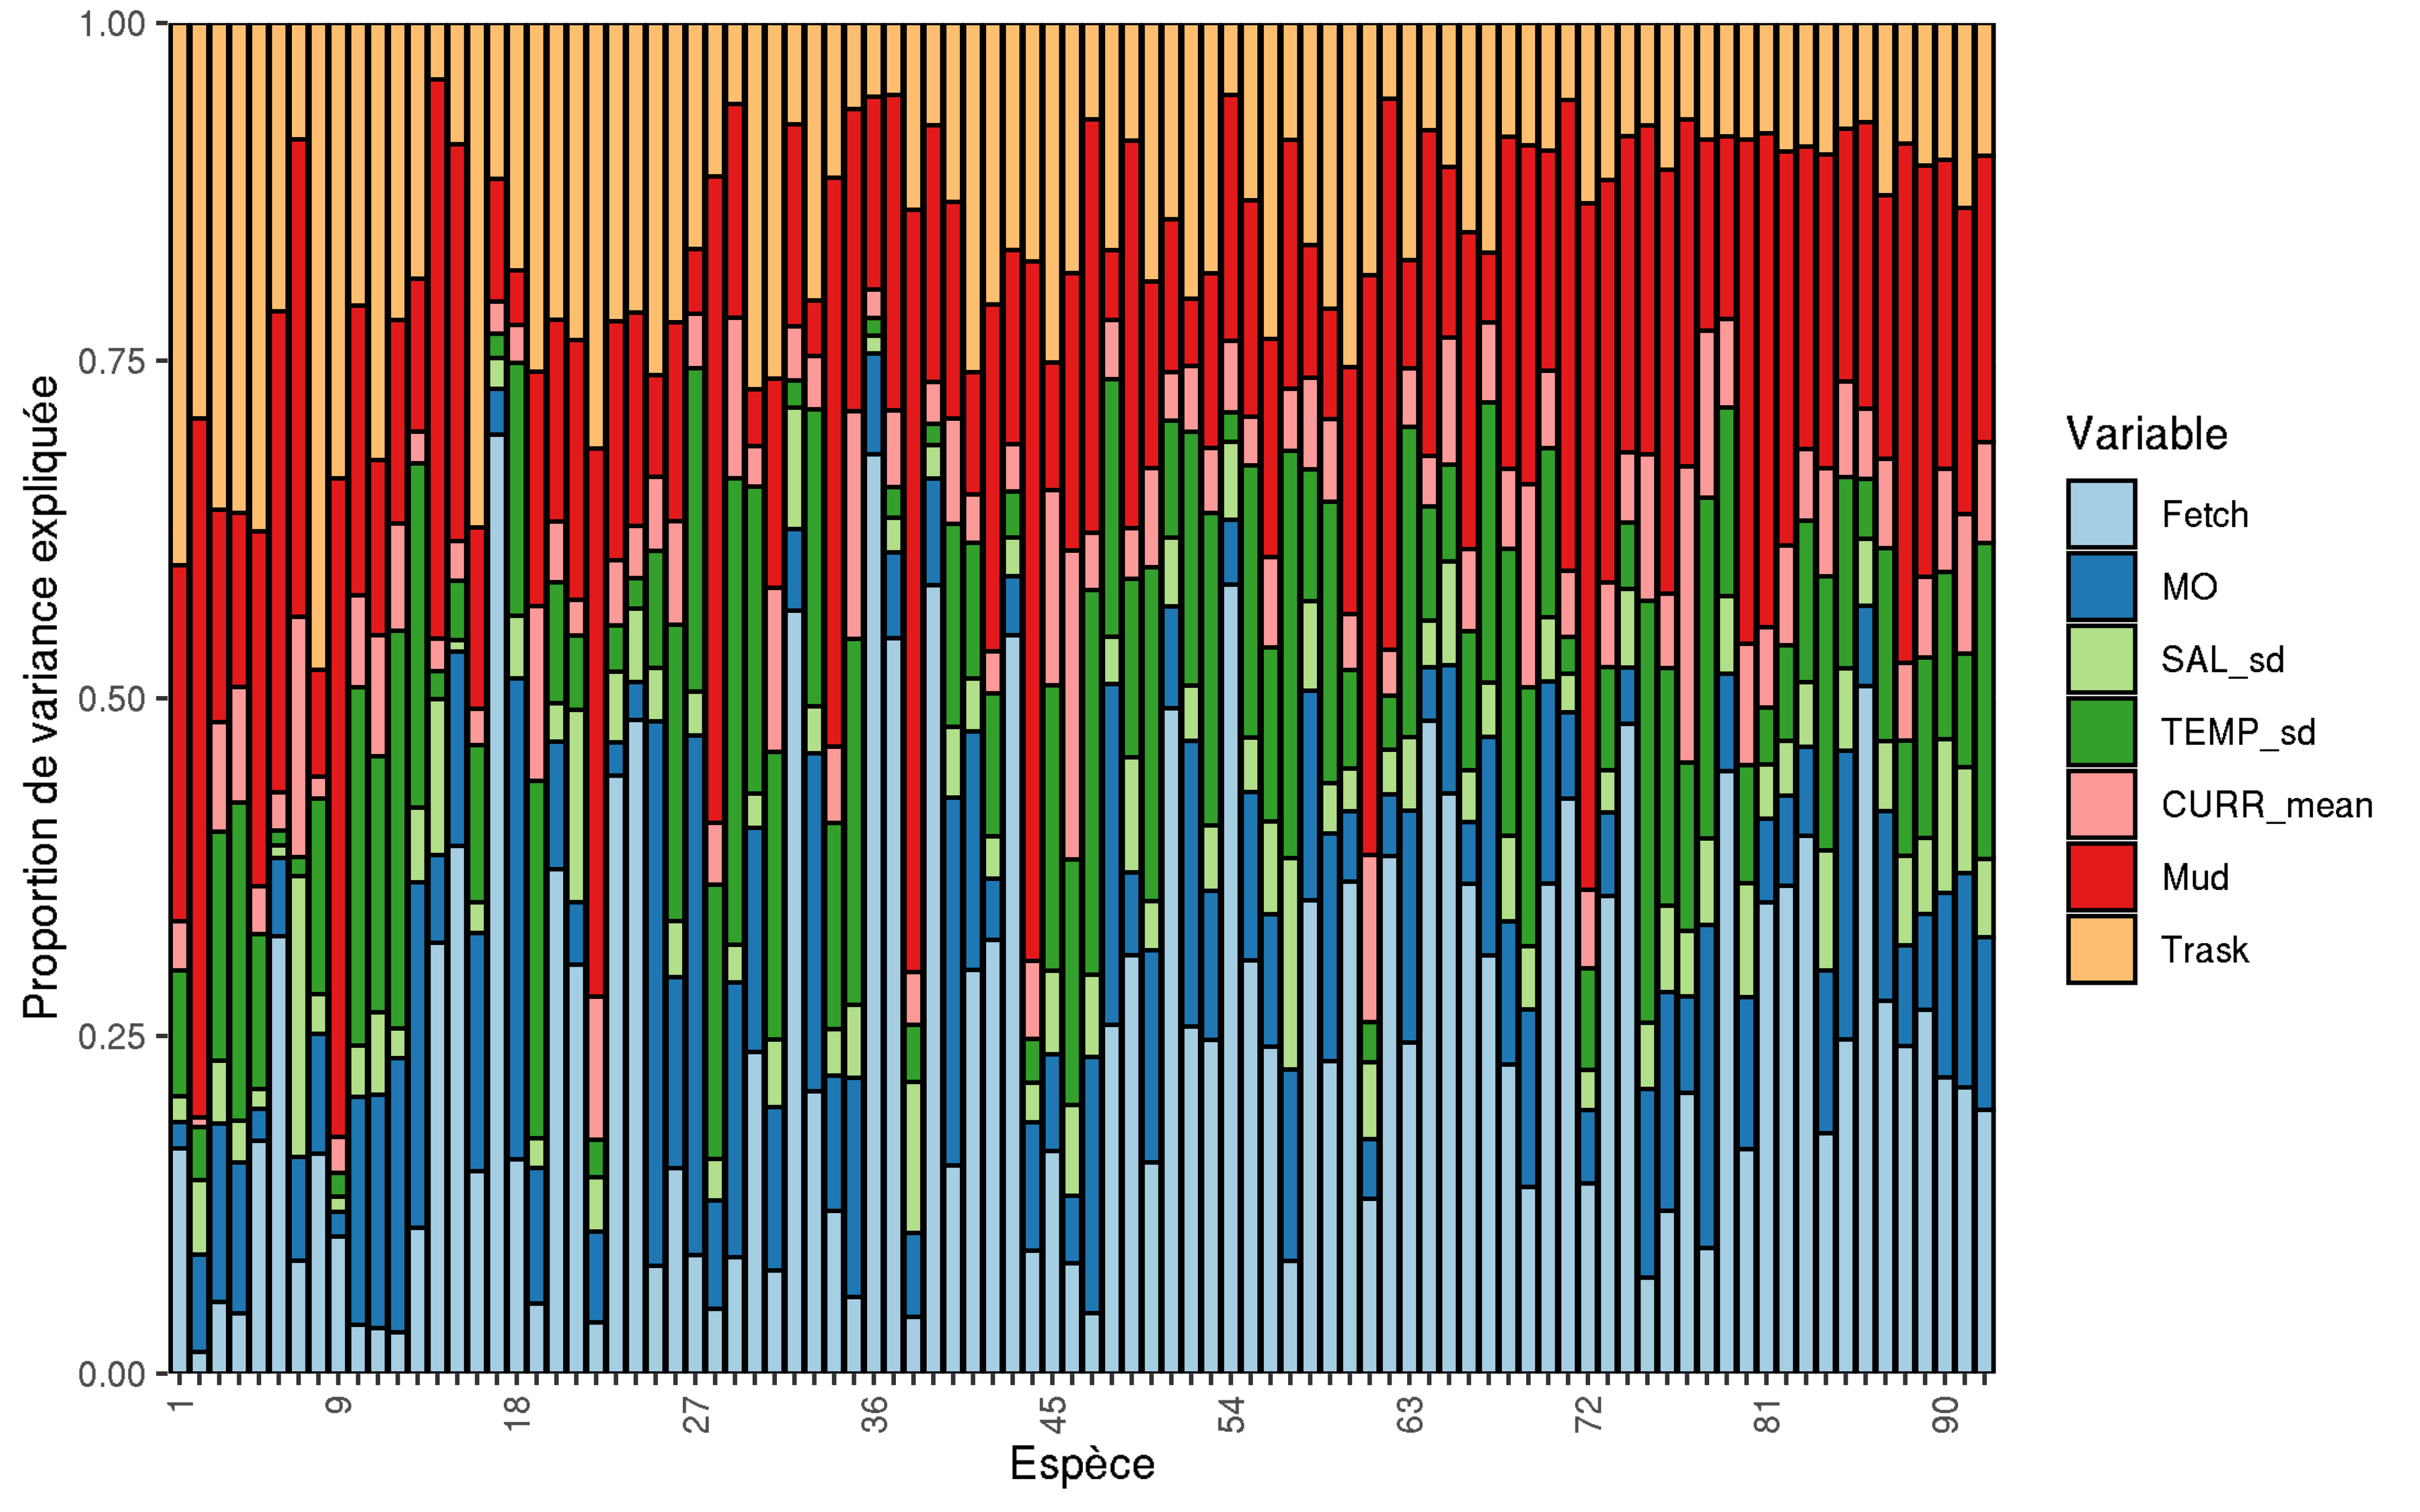
\includegraphics{figures/VP-HMSC-Var-Part-plot-1.png}
\caption{Partionnement de la variance de l'abondance des 92 taxons de
polychètes expliquée par les différentes variables environnementales du
modèle \emph{HMSC\_reg}. Les espèces sont classées par ordre décroissant
de \emph{SR\textsuperscript{2}} (voir
\cref{tbl:sp})}\label{fig:varpartreg}
}
\end{figure}

\begin{figure}
\hypertarget{fig:varpartsamp}{%
\centering
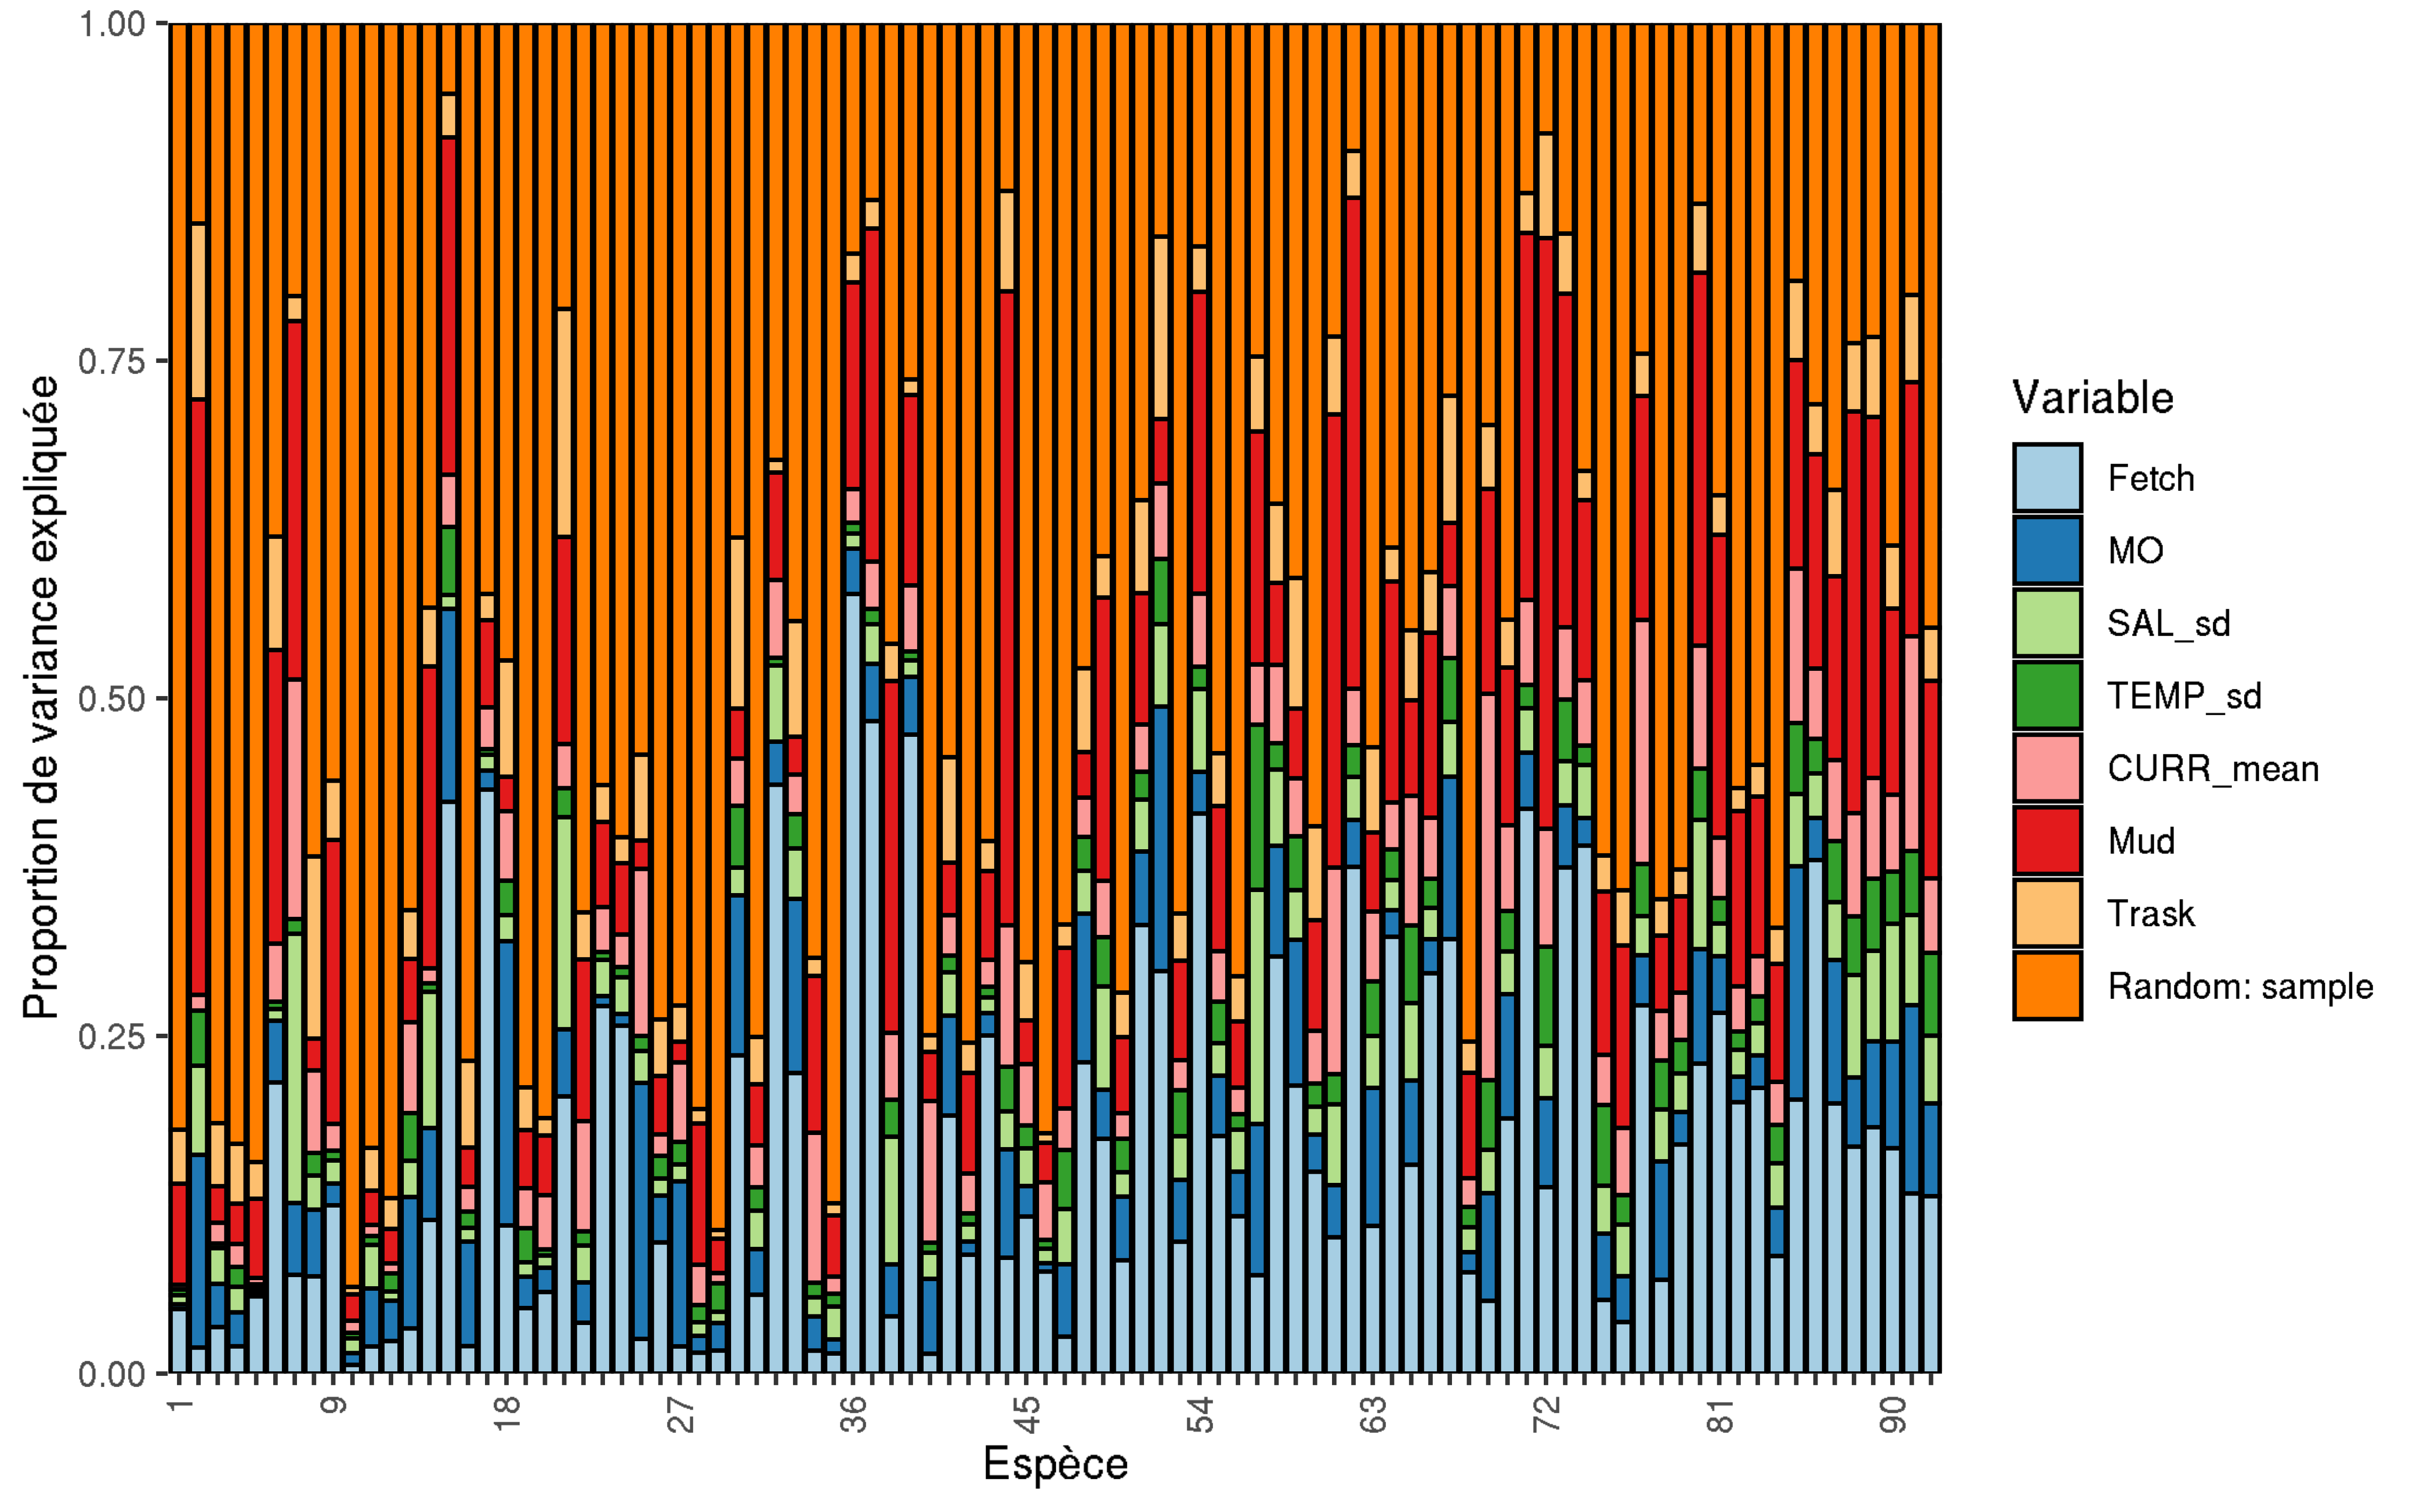
\includegraphics{figures/VP-HMSC-Var-Part-plot-2.png}
\caption{Partionnement de la variance de l'abondance des 92 taxons de
polychètes expliquée par les différentes variables environnementales du
modèle \emph{HMSC\_samp}. Les espèces sont classées par ordre
décroissant de \emph{SR\textsuperscript{2}} (voir
\cref{tbl:sp})}\label{fig:varpartsamp}
}
\end{figure}

\begin{figure}
\hypertarget{fig:varparthier}{%
\centering
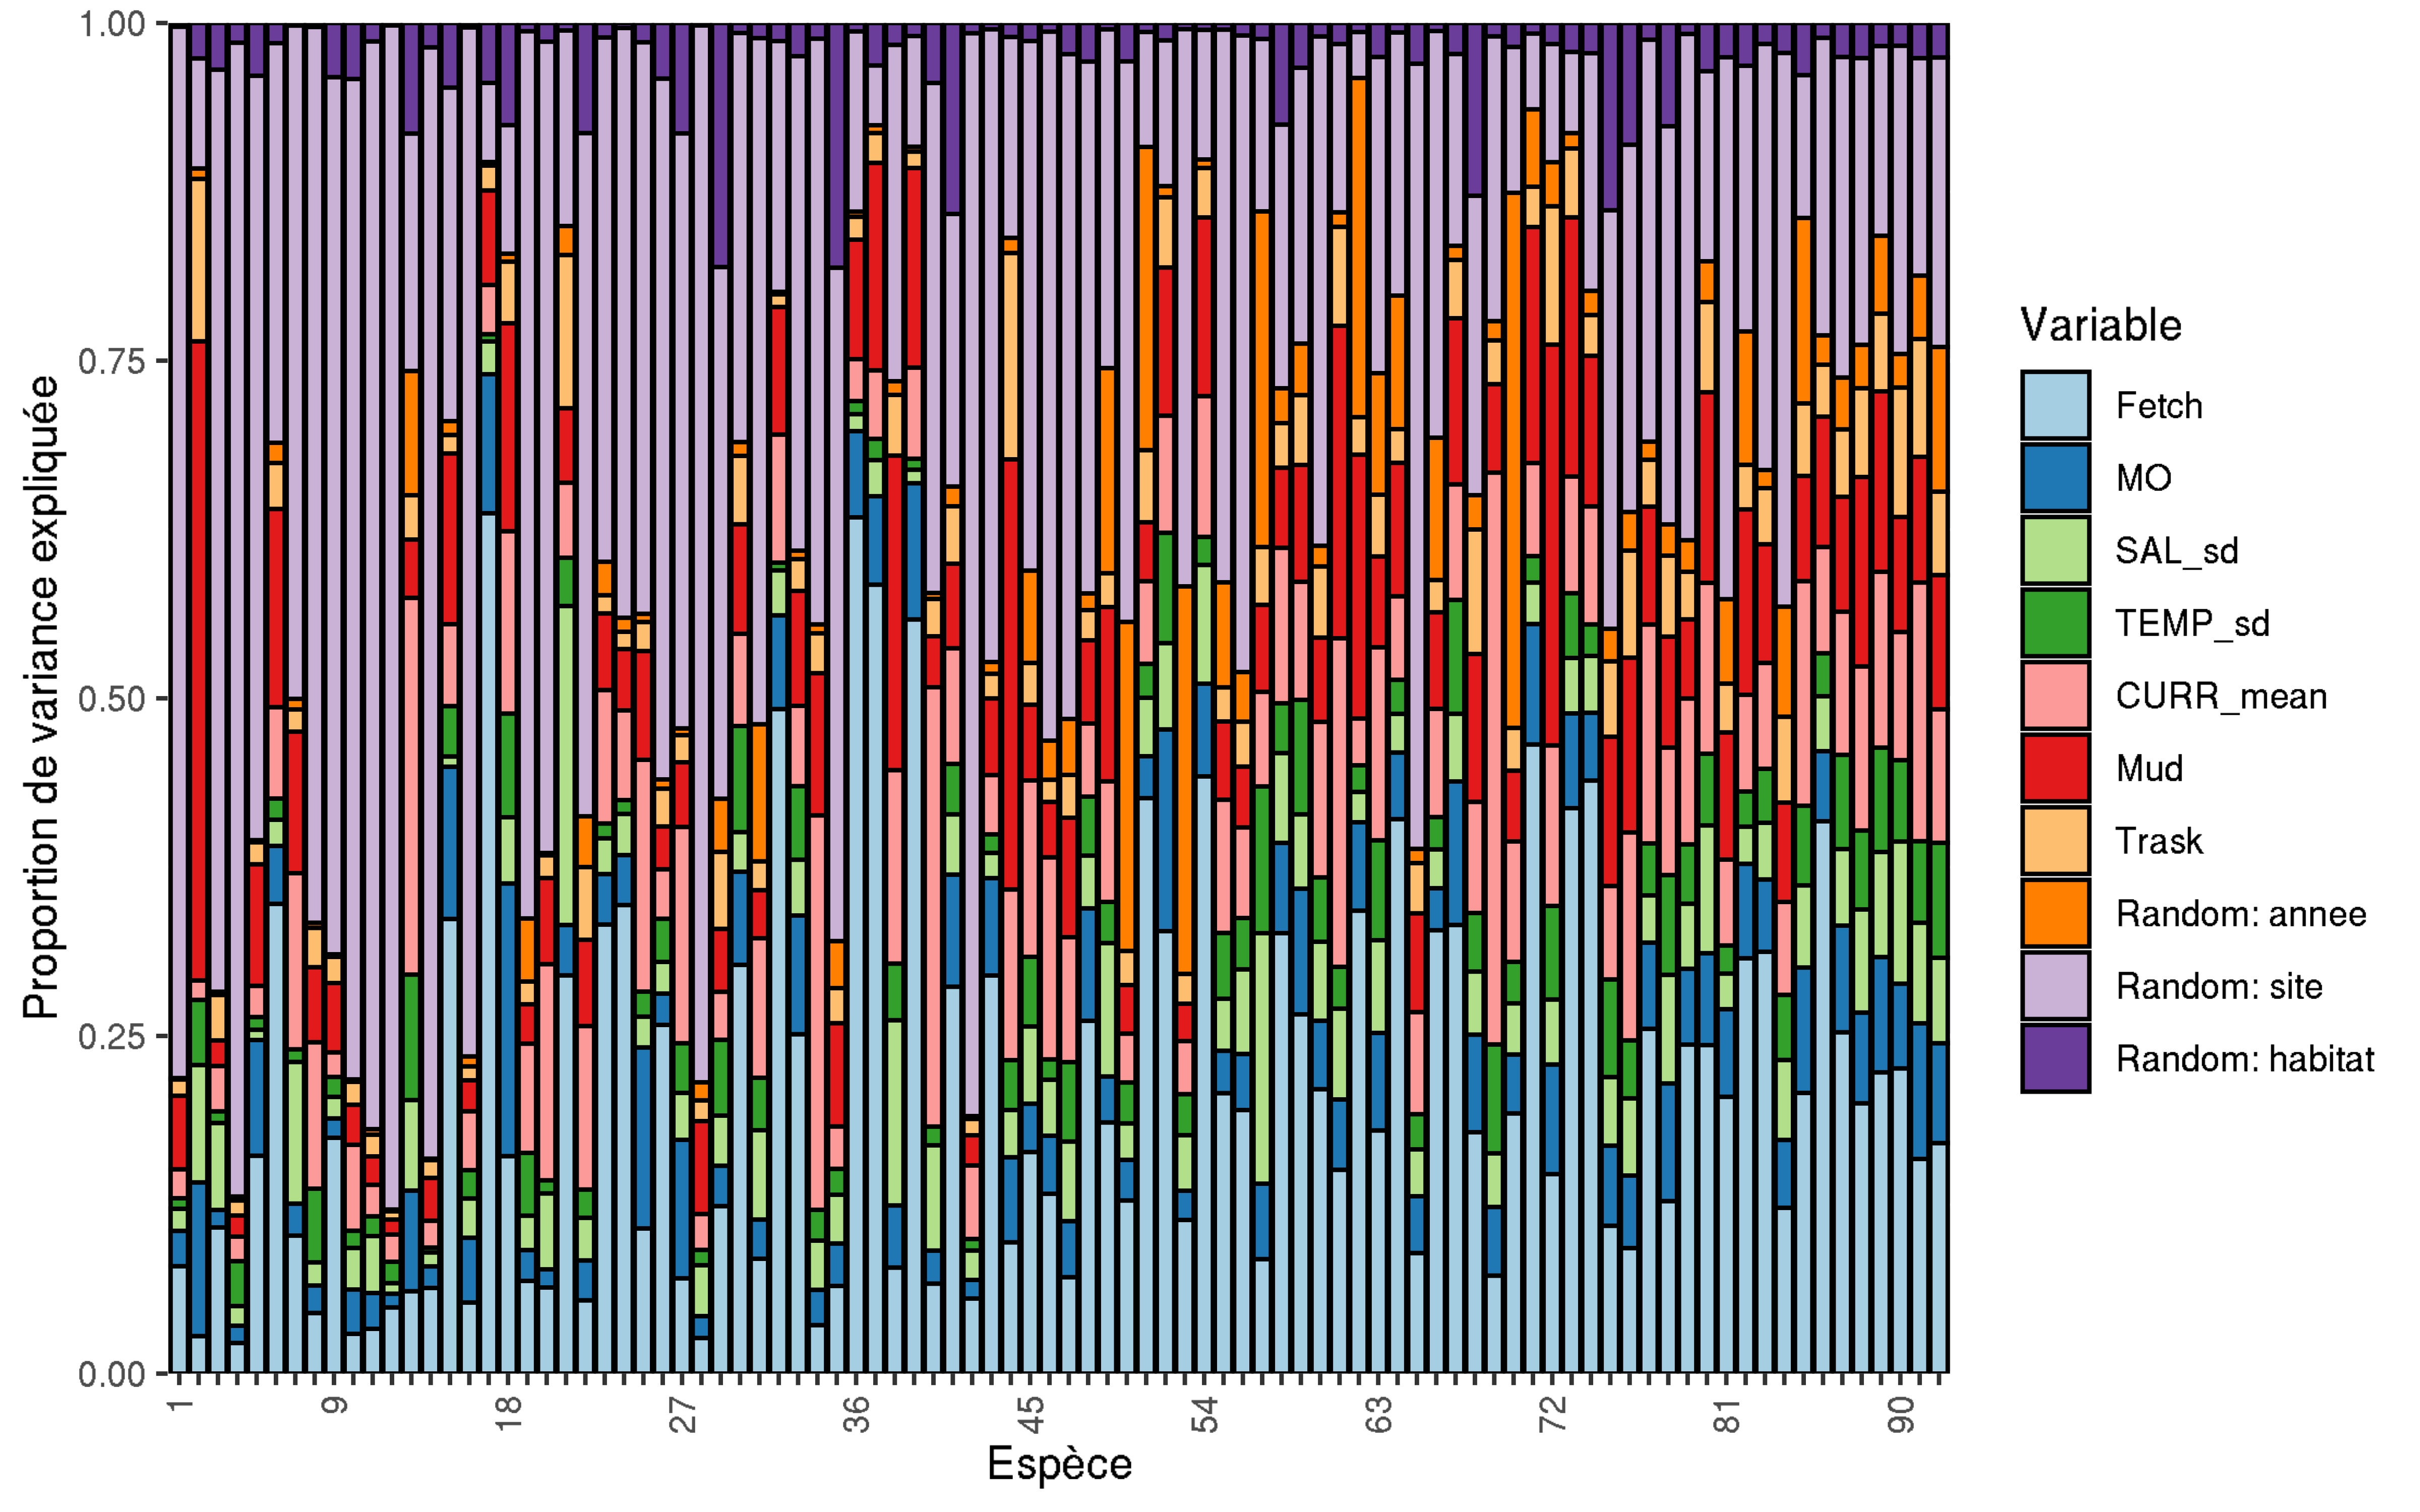
\includegraphics{figures/VP-HMSC-Var-Part-plot-3.png}
\caption{Partionnement de la variance de l'abondance des 92 taxons de
polychètes expliquée par les différentes variables environnementales du
modèle \emph{HMSC\_hier}. Les espèces sont classées par ordre
décroissant de \emph{SR\textsuperscript{2}} (voir
\cref{tbl:sp})}\label{fig:varparthier}
}
\end{figure}

\hypertarget{espuxe8ces-de-polychuxe8tes}{%
\subsection{Espèces de polychètes}\label{espuxe8ces-de-polychuxe8tes}}

{\small
\begin{longtable}[]{@{}rlll@{}}
\caption{Tableau de résumant les propriétés de la communauté des
Polychètes. Les numéros correspondent à ceux des figures des effets
environnementaux et du partionnement de variance, les espèces sont
ordonnées par \emph{SR\textsuperscript{2}} moyen décroissant. Les status
trophiques ont été confirmés par l'un de nos experts.
\label{tbl:sp}}\tabularnewline
\toprule
N° & specie & Status trophique & habitat\tabularnewline
\midrule
\endfirsthead
\toprule
N° & specie & Status trophique & habitat\tabularnewline
\midrule
\endhead
1 & Notomastus latericeus & Déposivore & Sédiment +
Herbier\tabularnewline
2 & Nephtys cirrosa & Prédateur/Charognard & Sédiment +
Herbier\tabularnewline
3 & Lumbrineris spp. & Prédateur/Charognard & Sédiment +
Herbier\tabularnewline
4 & Aonides oxycephala & Déposivore & Sédiment + Herbier\tabularnewline
5 & Euclymene spp. & Déposivore & Sédiment + Herbier\tabularnewline
6 & Glycera tridactyla & Prédateur/Charognard & Sédiment +
Herbier\tabularnewline
7 & Owenia fusiformis & Déposivore & Sédiment + Herbier\tabularnewline
8 & Lysidice unicornis & Prédateur/Charognard & Sédiment +
Herbier\tabularnewline
9 & Magelona filiformis & Déposivore & Sédiment\tabularnewline
10 & Platynereis dumerilii & Brouteur & Sédiment +
Herbier\tabularnewline
11 & Cirriformia tentaculata & Déposivore & Sédiment +
Herbier\tabularnewline
12 & Perinereis cultrifera & Brouteur & Sédiment +
Herbier\tabularnewline
13 & Heteromastus filiformis & Déposivore & Sédiment +
Herbier\tabularnewline
14 & Leiochone leiopygos & Déposivore & Sédiment +
Herbier\tabularnewline
15 & Scoloplos (Scoloplos) armiger & Déposivore & Sédiment +
Herbier\tabularnewline
16 & Polycirrus spp. & Déposivore & Sédiment + Herbier\tabularnewline
17 & Melinna palmata & Déposivore & Sédiment + Herbier\tabularnewline
18 & Pholoe inornata & Prédateur/Charognard & Sédiment +
Herbier\tabularnewline
19 & Caulleriella alata & Déposivore & Sédiment + Herbier\tabularnewline
20 & Acromegalomma spp. & Suspensivore & Sédiment +
Herbier\tabularnewline
21 & Eteone longa & Prédateur/Charognard & Sédiment +
Herbier\tabularnewline
22 & Sigalion mathildae & Prédateur/Charognard & Sédiment\tabularnewline
23 & Chaetozone spp. & Déposivore & Sédiment + Herbier\tabularnewline
24 & Chaetozone gibber & Déposivore & Sédiment + Herbier\tabularnewline
25 & Malmgrenia arenicolae & Prédateur/Charognard & Sédiment +
Herbier\tabularnewline
26 & Hilbigneris gracilis & Déposivore/Prédateur/Charognard & Sédiment +
Herbier\tabularnewline
27 & Scalibregma celticum & Déposivore & Herbier\tabularnewline
28 & Spio spp. & Déposivore & Sédiment + Herbier\tabularnewline
29 & Malacoceros girardi & Déposivore & Herbier\tabularnewline
30 & Harmothoe spinifera & Prédateur/Charognard & Sédiment +
Herbier\tabularnewline
31 & Caulleriella bioculata & Déposivore & Sédiment +
Herbier\tabularnewline
32 & Aponuphis bilineata & Prédateur/Charognard & Sédiment +
Herbier\tabularnewline
33 & Piromis eruca & Déposivore & Herbier\tabularnewline
34 & Phyllodoce mucosa & Prédateur/Charognard & Sédiment +
Herbier\tabularnewline
35 & Neanthes acuminata & Omnivore & Herbier\tabularnewline
36 & Ampharete spp. & Déposivore & Sédiment + Herbier\tabularnewline
37 & Paradoneis armata & Déposivore & Sédiment + Herbier\tabularnewline
38 & Scolelepis spp. & Déposivore & Sédiment + Herbier\tabularnewline
39 & Poecilochaetus serpens & Déposivore & Sédiment +
Herbier\tabularnewline
40 & Sthenelais boa & Prédateur/Charognard & Sédiment +
Herbier\tabularnewline
41 & Harmothoe impar & Prédateur/Charognard & Herbier\tabularnewline
42 & Marphysa bellii & Prédateur/Charognard & Sédiment +
Herbier\tabularnewline
43 & Lanice conchilega & Déposivore & Sédiment + Herbier\tabularnewline
44 & Orbinia latreillii & Déposivore & Sédiment + Herbier\tabularnewline
45 & Schistomeringos rudolphi & Omnivore & Sédiment +
Herbier\tabularnewline
46 & Syllis garciai & Omnivore & Sédiment + Herbier\tabularnewline
47 & Capitella capitata & Déposivore & Sédiment + Herbier\tabularnewline
48 & Terebellides spp. & Déposivore & Herbier\tabularnewline
49 & Pygospio elegans & Déposivore & Sédiment + Herbier\tabularnewline
50 & Scoletoma spp. & Prédateur/Charognard & Sédiment +
Herbier\tabularnewline
51 & Prionospio spp. & Déposivore & Sédiment + Herbier\tabularnewline
52 & Eunice vittata & Prédateur/Charognard & Sédiment +
Herbier\tabularnewline
53 & Macroclymene santanderensis & Déposivore & Sédiment +
Herbier\tabularnewline
54 & Lagis koreni & Déposivore & Sédiment + Herbier\tabularnewline
55 & Polydora spp. & Déposivore & Sédiment + Herbier\tabularnewline
56 & Protodorvillea kefersteini & Omnivore & Sédiment +
Herbier\tabularnewline
57 & Capitella minima & Déposivore & Sédiment + Herbier\tabularnewline
58 & Eupolymnia nebulosa & Déposivore & Sédiment +
Herbier\tabularnewline
59 & Pista spp. & Déposivore & Sédiment + Herbier\tabularnewline
60 & Eumida spp. & Prédateur/Charognard & Sédiment +
Herbier\tabularnewline
61 & Spiophanes bombyx & Déposivore & Sédiment + Herbier\tabularnewline
62 & Paradoneis lyra & Déposivore & Sédiment + Herbier\tabularnewline
63 & Amphitritides gracilis & Déposivore & Sédiment +
Herbier\tabularnewline
64 & Parexogone hebes & Omnivore & Sédiment + Herbier\tabularnewline
65 & Arenicola marina & Déposivore & Sédiment + Herbier\tabularnewline
66 & Nicomache lumbricalis & Déposivore & Sédiment +
Herbier\tabularnewline
67 & Leodice harassii & Prédateur/Charognard & Herbier\tabularnewline
68 & Microspio spp. & Déposivore & Sédiment + Herbier\tabularnewline
69 & Mysta picta & Prédateur/Charognard & Sédiment +
Herbier\tabularnewline
70 & Cirratulidae spp. & Déposivore & Sédiment + Herbier\tabularnewline
71 & Phyllodoce lineata & Prédateur/Charognard & Sédiment +
Herbier\tabularnewline
72 & Nephtys spp. & Prédateur/Charognard & Sédiment +
Herbier\tabularnewline
73 & Hypereteone foliosa & Prédateur/Charognard &
Sédiment\tabularnewline
74 & Petaloproctus terricolus & Déposivore & Sédiment +
Herbier\tabularnewline
75 & Malacoceros spp. & Déposivore & Herbier\tabularnewline
76 & Malacoceros fuliginosus & Déposivore & Sédiment +
Herbier\tabularnewline
77 & Paraonidae spp. & Déposivore & Sédiment + Herbier\tabularnewline
78 & Syllis spp. & Omnivore & Herbier\tabularnewline
79 & Sphaerosyllis spp. & Omnivore & Sédiment + Herbier\tabularnewline
80 & Malmgrenia spp. & Prédateur/Charognard & Sédiment +
Herbier\tabularnewline
81 & Phyllodoce laminosa & Prédateur/Charognard & Sédiment +
Herbier\tabularnewline
82 & Maldanidae spp. & Déposivore & Sédiment + Herbier\tabularnewline
83 & Sabella pavonina & Suspensivore & Sédiment + Herbier\tabularnewline
84 & Nereis spp. & Omnivore & Sédiment + Herbier\tabularnewline
85 & Psamathe fusca & Prédateur/Charognard & Sédiment +
Herbier\tabularnewline
86 & Chaetozone zetlandica & Déposivore & Sédiment +
Herbier\tabularnewline
87 & Eumida parva & Prédateur/Charognard & Sédiment +
Herbier\tabularnewline
88 & Orbinia sertulata & Déposivore & Sédiment + Herbier\tabularnewline
89 & Goniada spp. & Prédateur/Charognard & Sédiment +
Herbier\tabularnewline
90 & Glycera spp. & Prédateur/Charognard & Sédiment +
Herbier\tabularnewline
91 & Malmgrenia andreapolis & Prédateur/Charognard & Sédiment +
Herbier\tabularnewline
92 & Spirobranchus spp. & Suspensivore & Sédiment +
Herbier\tabularnewline
\bottomrule
\end{longtable}}\FloatBarrier


\hypertarget{ruxe9seaux-reconstruits-1}{%
\subsection{Réseaux reconstruits}\label{ruxe9seaux-reconstruits-1}}

\begin{figure}
\hypertarget{fig:netgllvm}{%
\centering
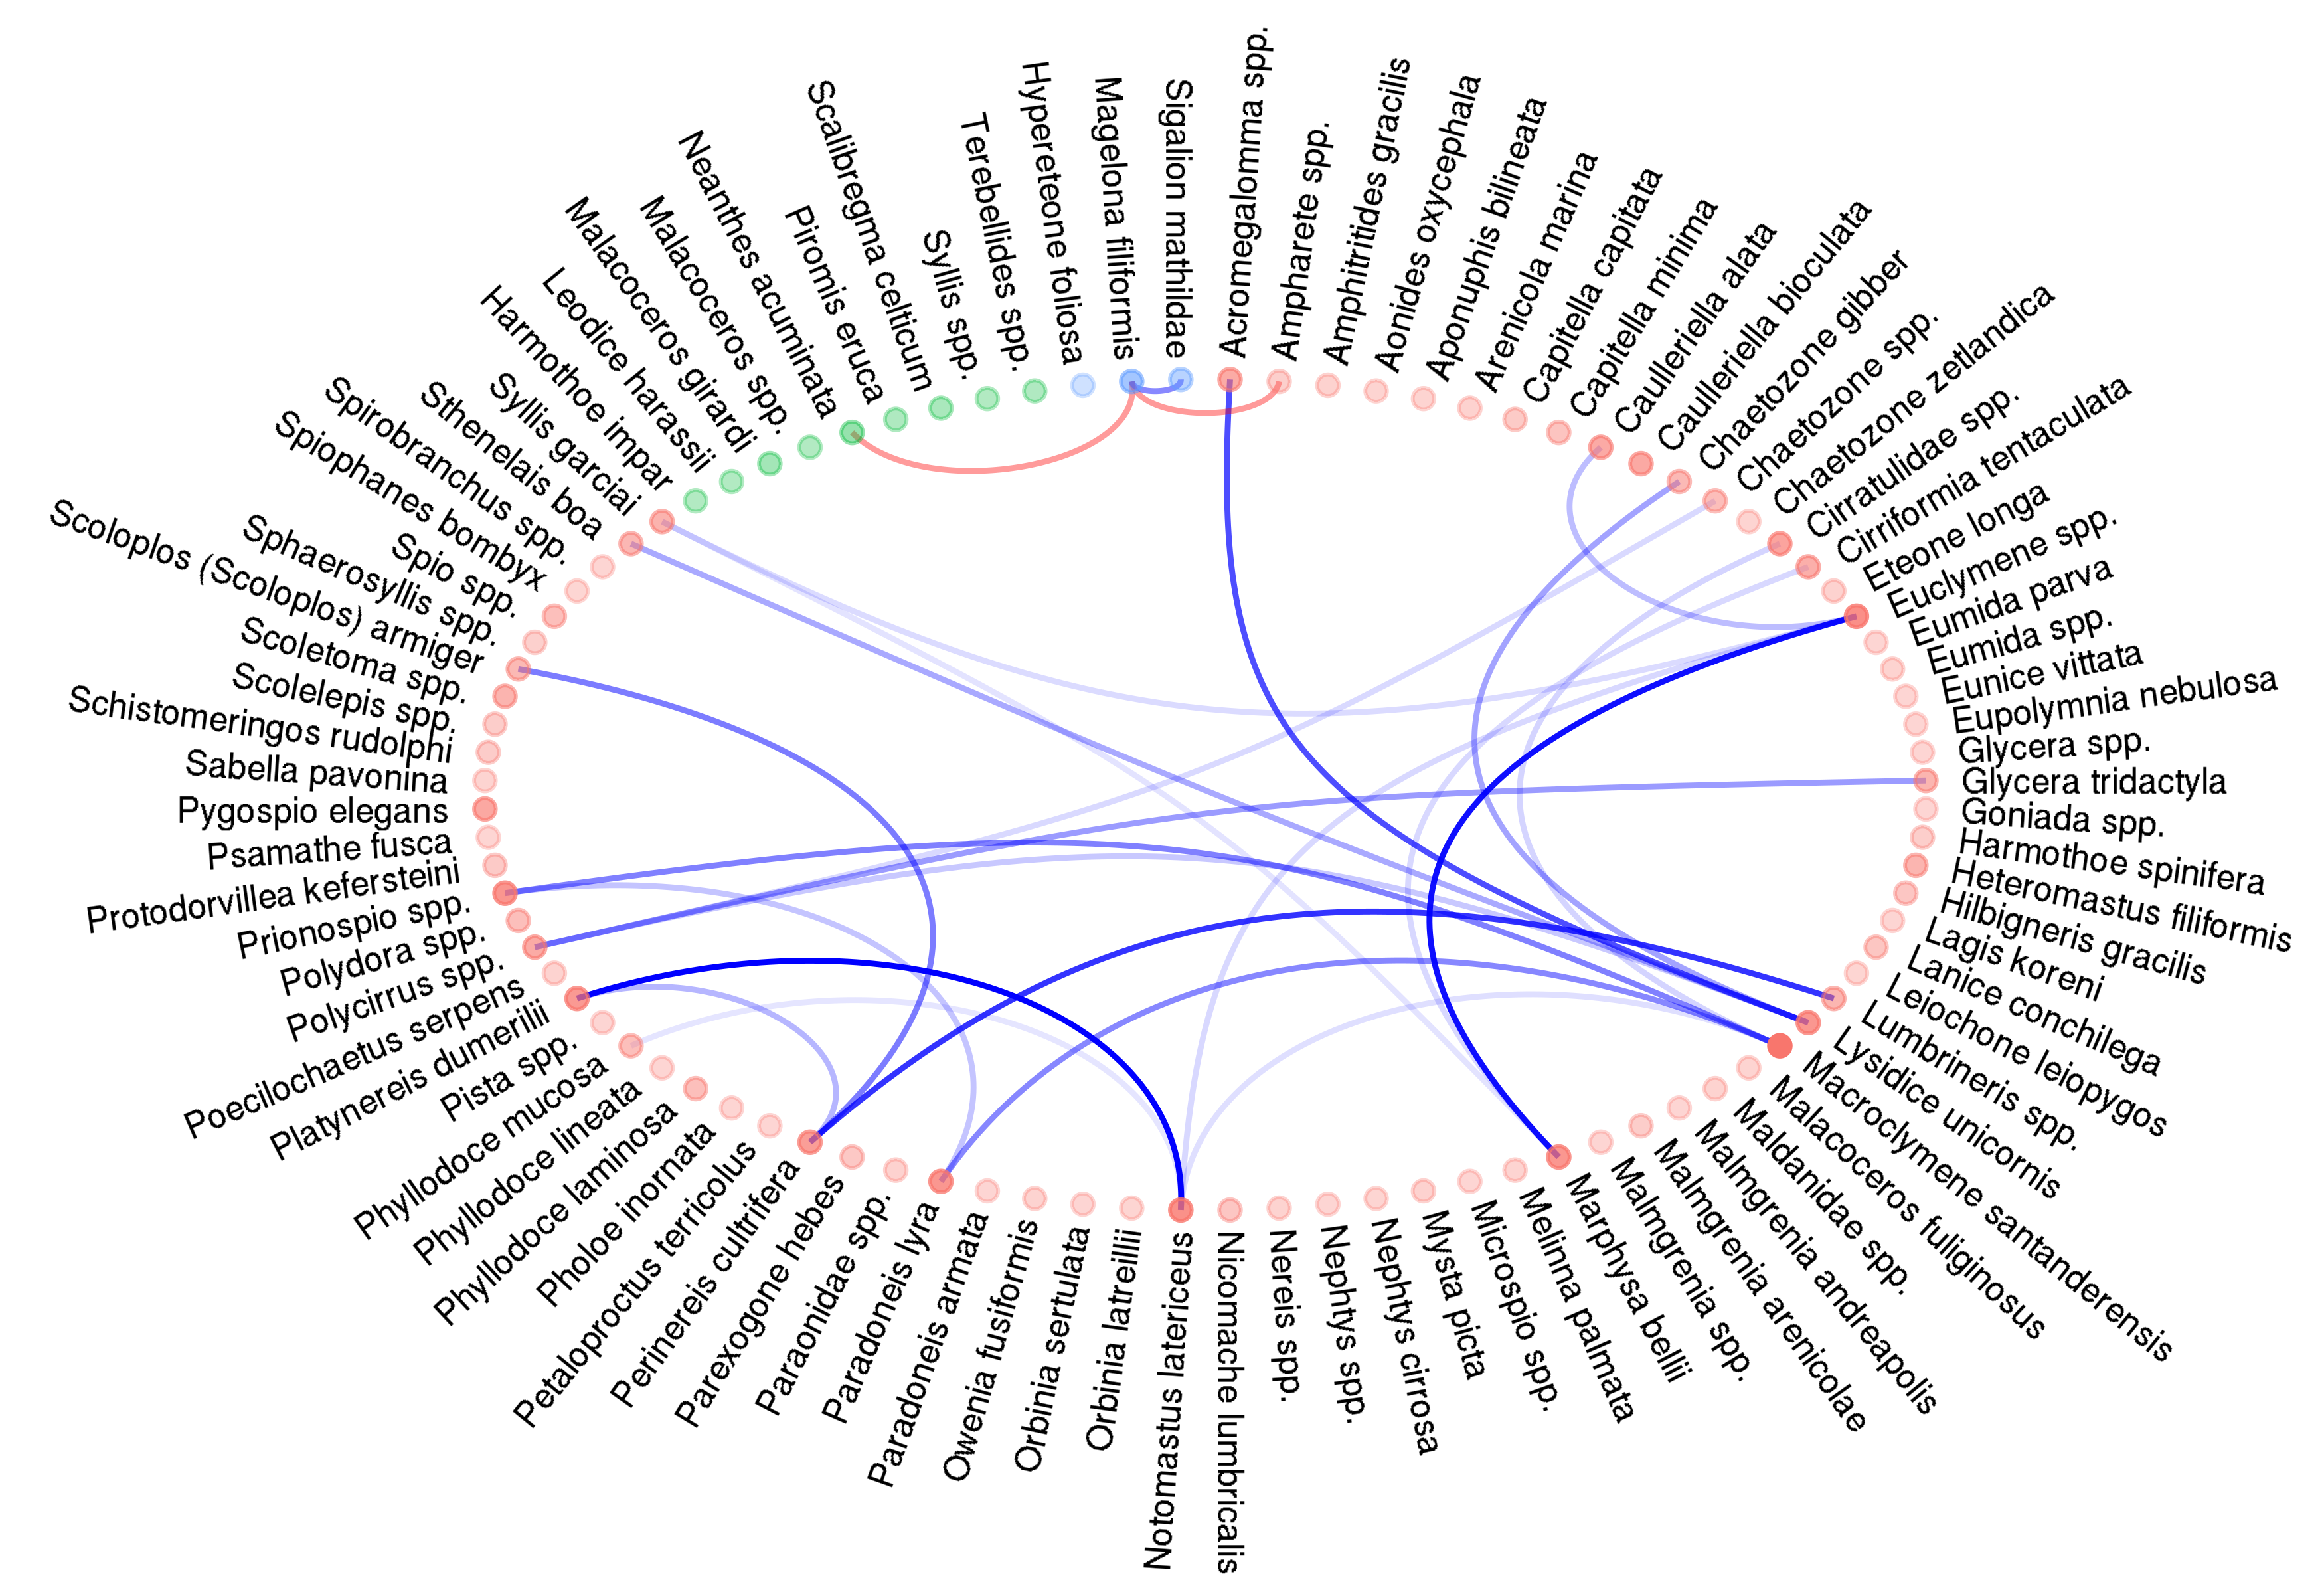
\includegraphics{figures/gllvm-network-1.png}
\caption{Réseau reconstruit présentant les probabilités d'interaction
inférées par \emph{EMtree} sur la base des corrélations résiduelles
associées à l'effet aléatoire du modèle \emph{GLLVM}. Les points rouges
représentent les taxa de polychètes retrouvés dans les deux habitats,
les verts retrouvés uniquement dans les herbiers et les bleus dans les
sédiments meubles. Seules les arrêtes ayant une probabilité supérieur à
\(0,2\) sont affichées. L'opacité des arrêtes est proportionnelle à leur
probabilité. L'opacité des points est proportionnelle à leur importance
dans le réseau}\label{fig:netgllvm}
}
\end{figure}

\begin{figure}
\hypertarget{fig:netpln}{%
\centering
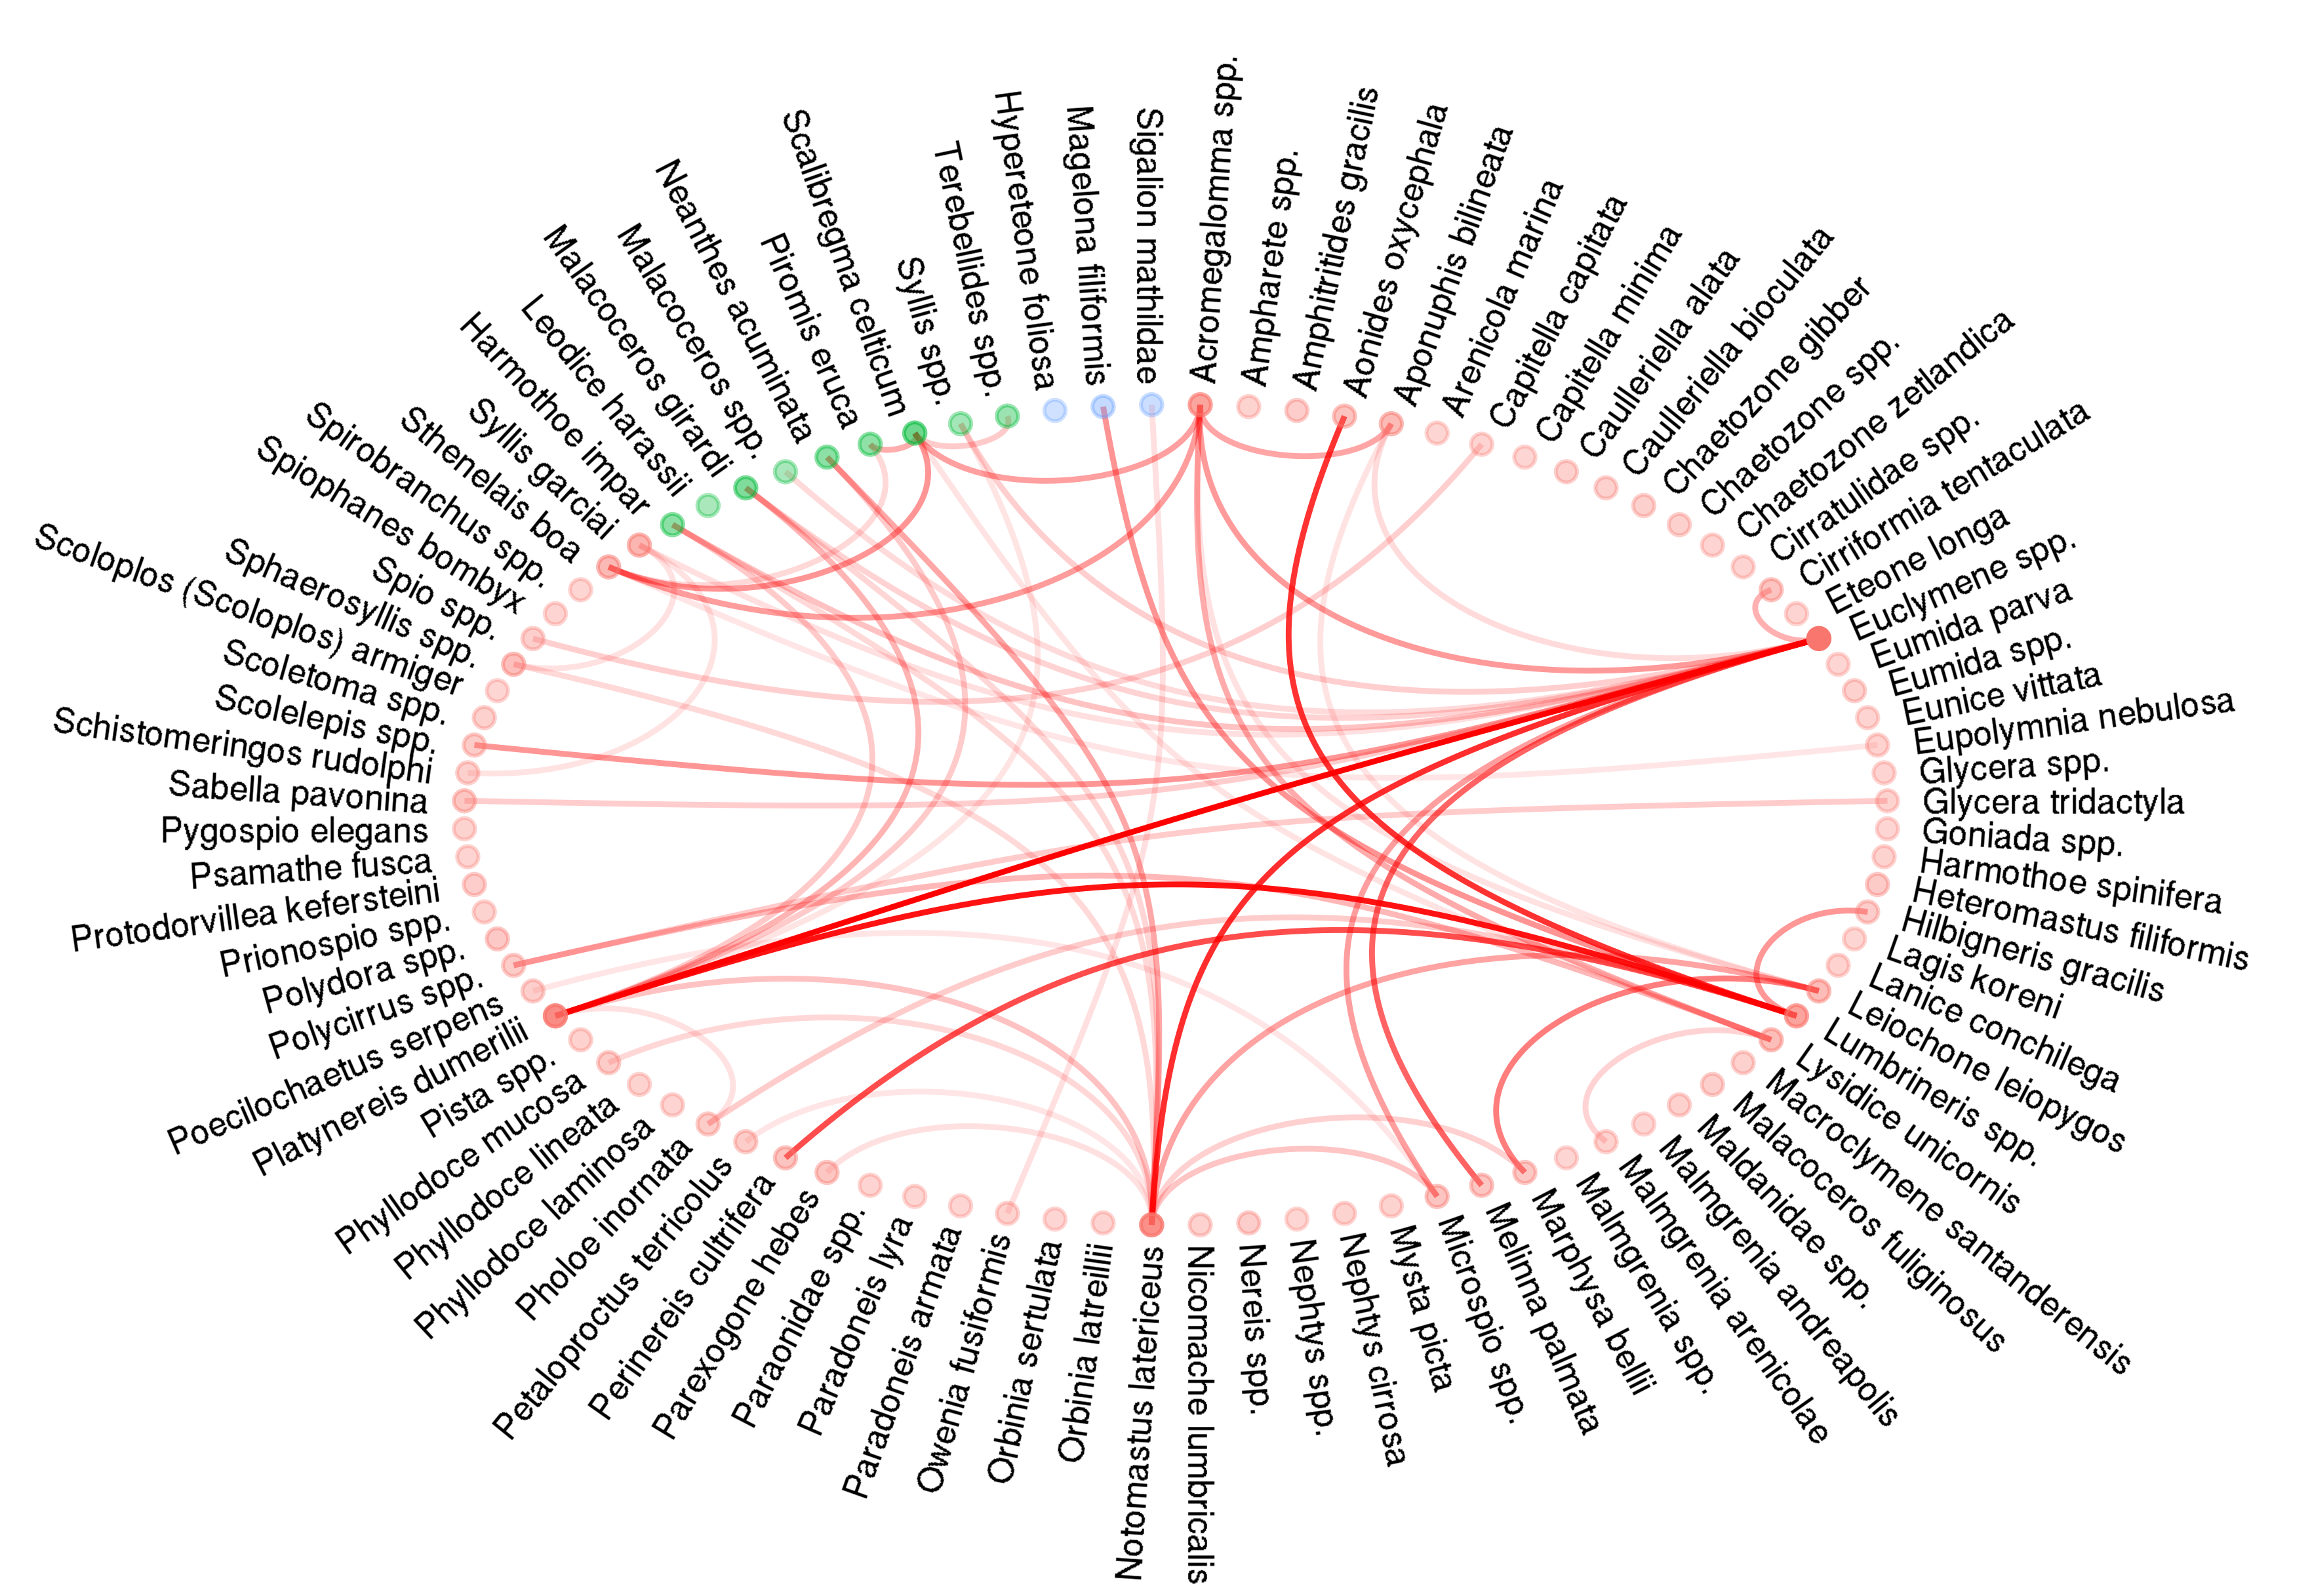
\includegraphics{figures/pln-network-1.png}
\caption{Réseau présentant les probabilités d'interaction inférées par
\emph{EMtree} sur la base des corrélations résiduelles associées à
l'effet aléatoire du modèle \emph{PLN}. Les points rouges représentent
les taxa de polychètes retrouvés dans les deux habitats, les verts
retrouvés uniquement dans les herbiers et les bleus dans les sédiments
meubles. Seules les arrêtes ayant une probabilité supérieur à \(0,2\)
sont affichées. L'opacité des arrêtes est proportionnelle à leur
probabilité. L'opacité des points est proportionnelle à leur importance
dans le réseau.}\label{fig:netpln}
}
\end{figure}

\begin{figure}
\hypertarget{fig:nethmscsamp}{%
\centering
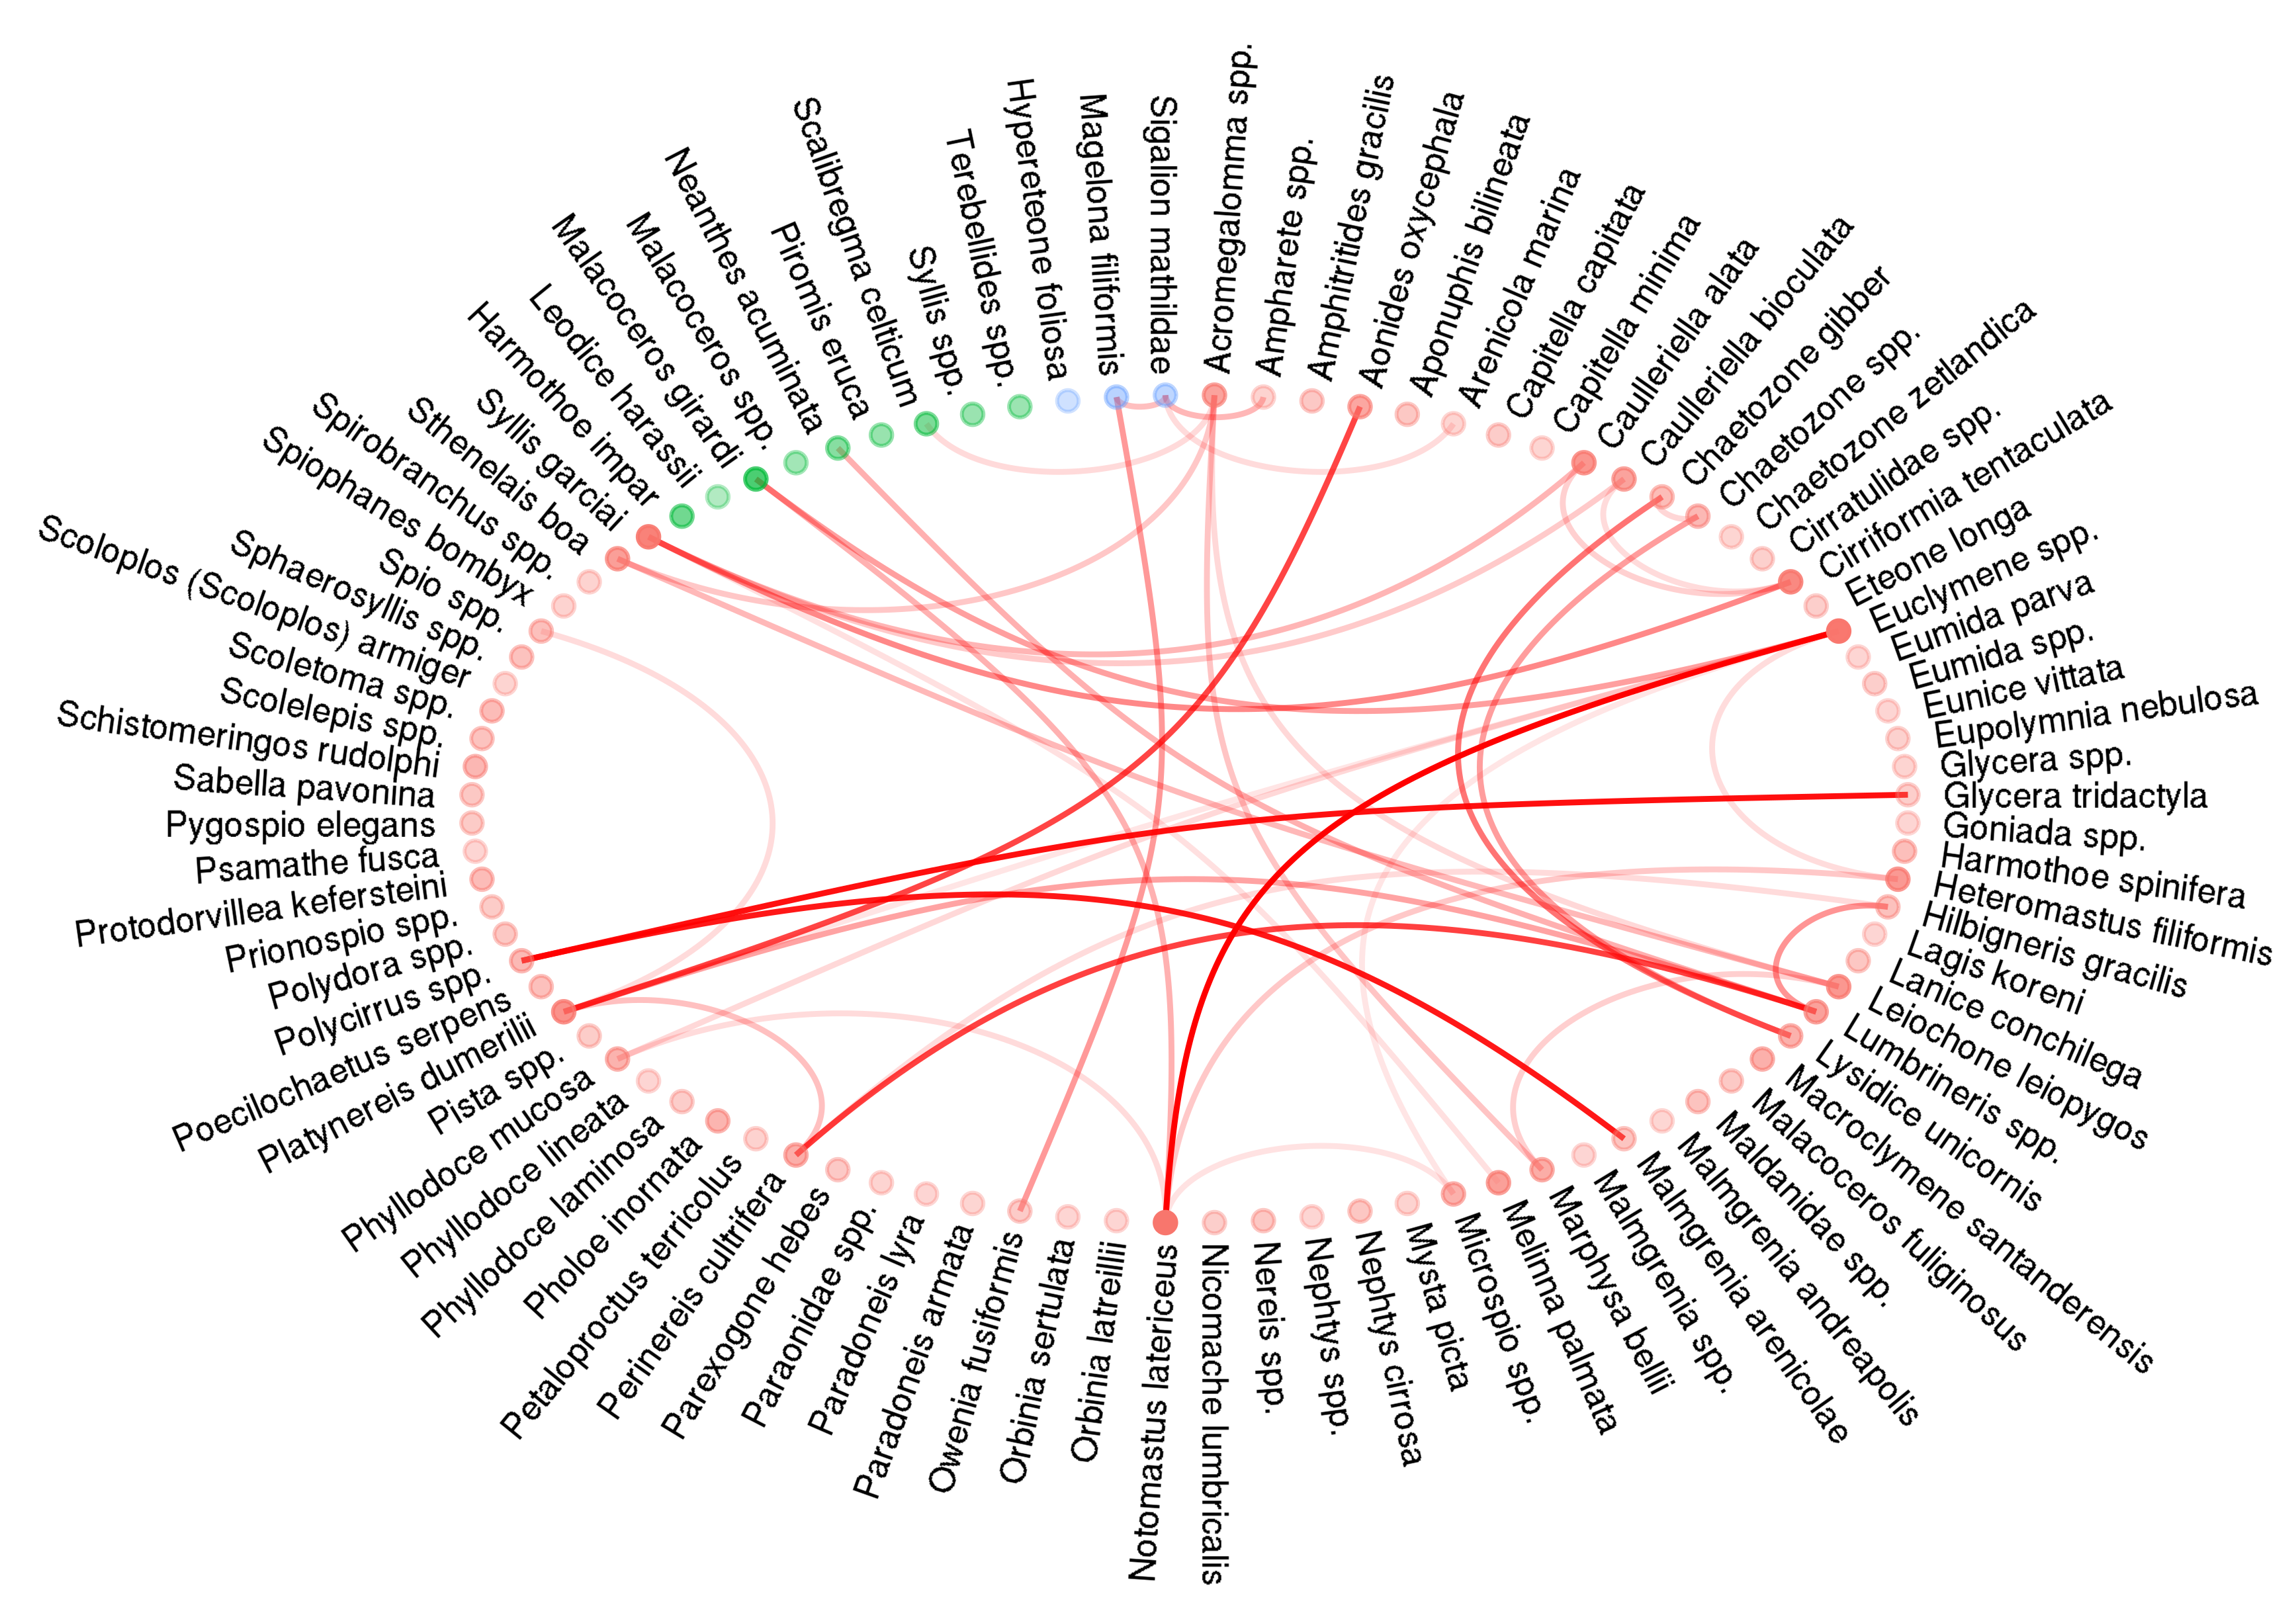
\includegraphics{figures/hmsc-samp-network-1.png}
\caption{Réseau reconstruit présentant les probabilités d'interaction
inférées par \emph{EMtree} sur la base des corrélations résiduelles
associées à l'effet aléatoire spatial du modèle \emph{HMSC\_hier}. Les
points rouges représentent les taxa de polychètes retrouvés dans les
deux habitats, les verts retrouvés uniquement dans les herbiers et les
bleus dans les sédiments meubles. Seules les arrêtes ayant une
probabilité supérieur à \(0,2\) sont affichées. L'opacité des arrêtes
est proportionnelle à leur probabilité. L'opacité des points est
proportionnelle à leur importance dans le
réseau.}\label{fig:nethmscsamp}
}
\end{figure}

\begin{figure}
\hypertarget{fig:nethmschiersite}{%
\centering
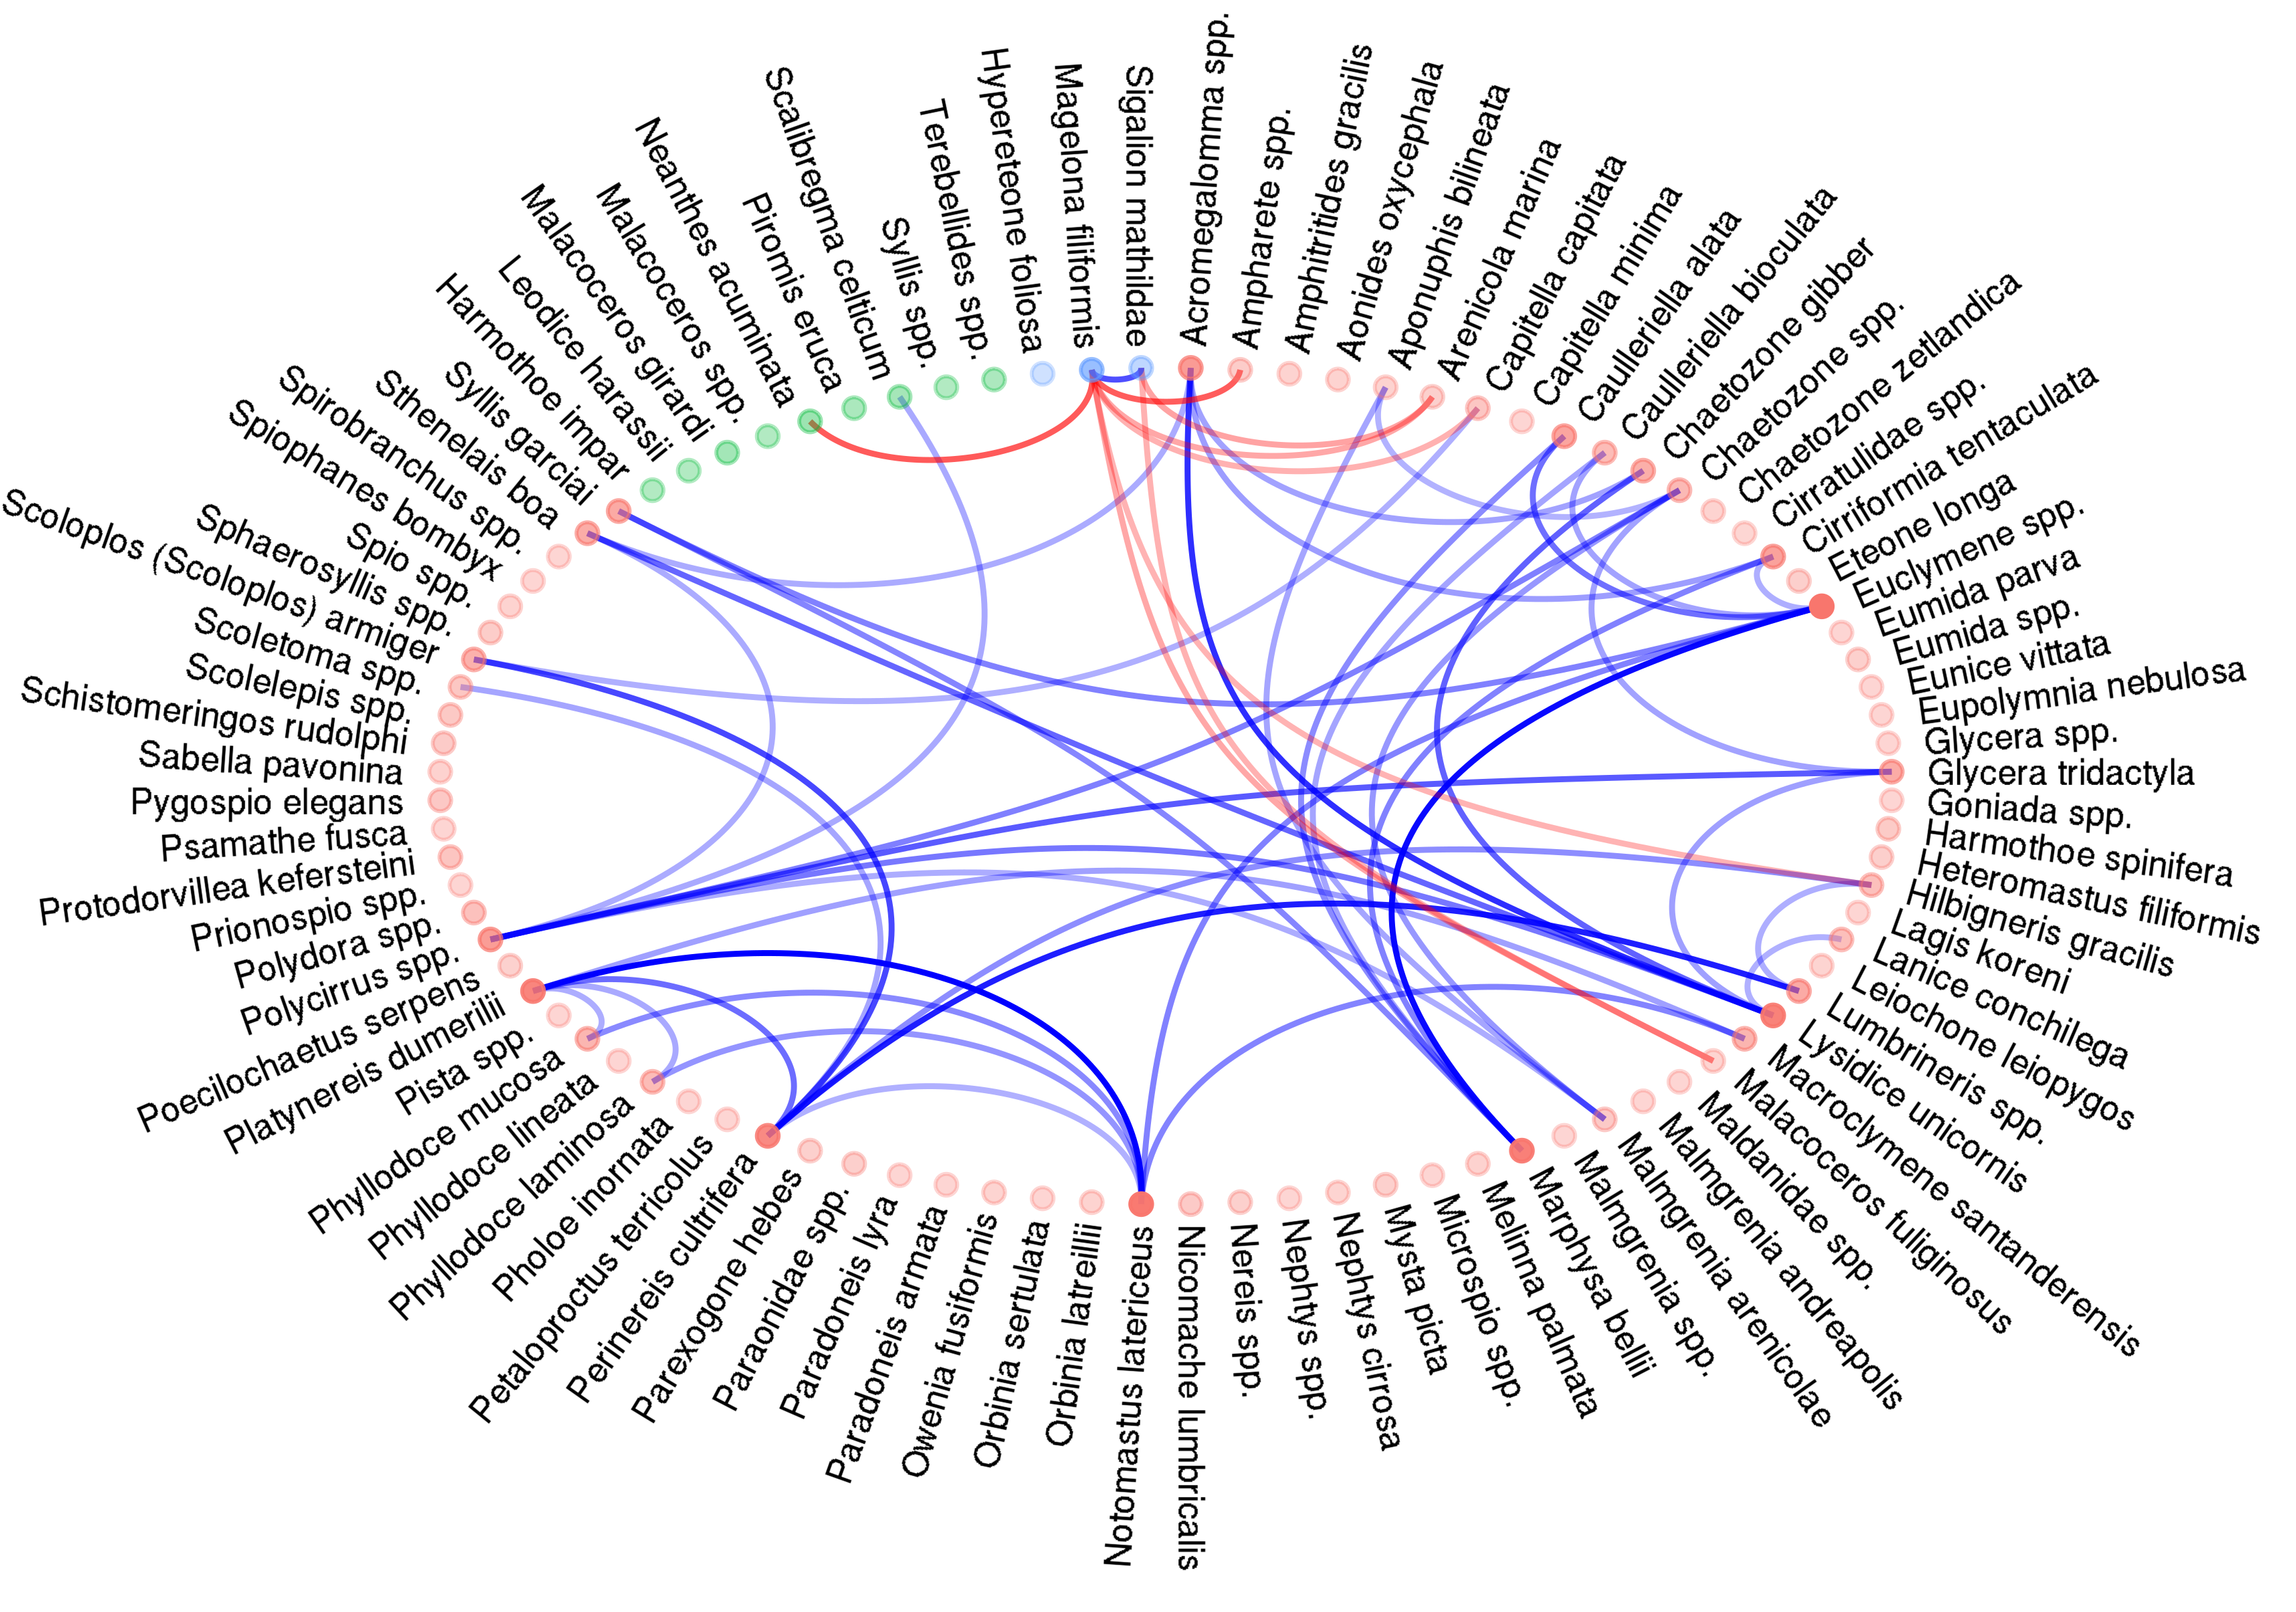
\includegraphics{figures/hmsc-hier-site-network-1.png}
\caption{Réseau reconstruit présentant les probabilités d'interaction
inférées par \emph{EMtree} sur la base des corrélations résiduelles
associées à l'effet aléatoire site du modèle \emph{HMSC\_hier}. Les
points rouges représentent les taxa de polychètes retrouvés dans les
deux habitats, les verts retrouvés uniquement dans les herbiers et les
bleus dans les sédiments meubles. Seules les arrêtes ayant une
probabilité supérieur à \(0,2\) sont affichées.L'opacité des arrêtes est
proportionnelle à leur probabilité. L'opacité des points est
proportionnelle à leur importance dans le
réseau.}\label{fig:nethmschiersite}
}
\end{figure}

\begin{figure}
\hypertarget{fig:nethmschierhab}{%
\centering
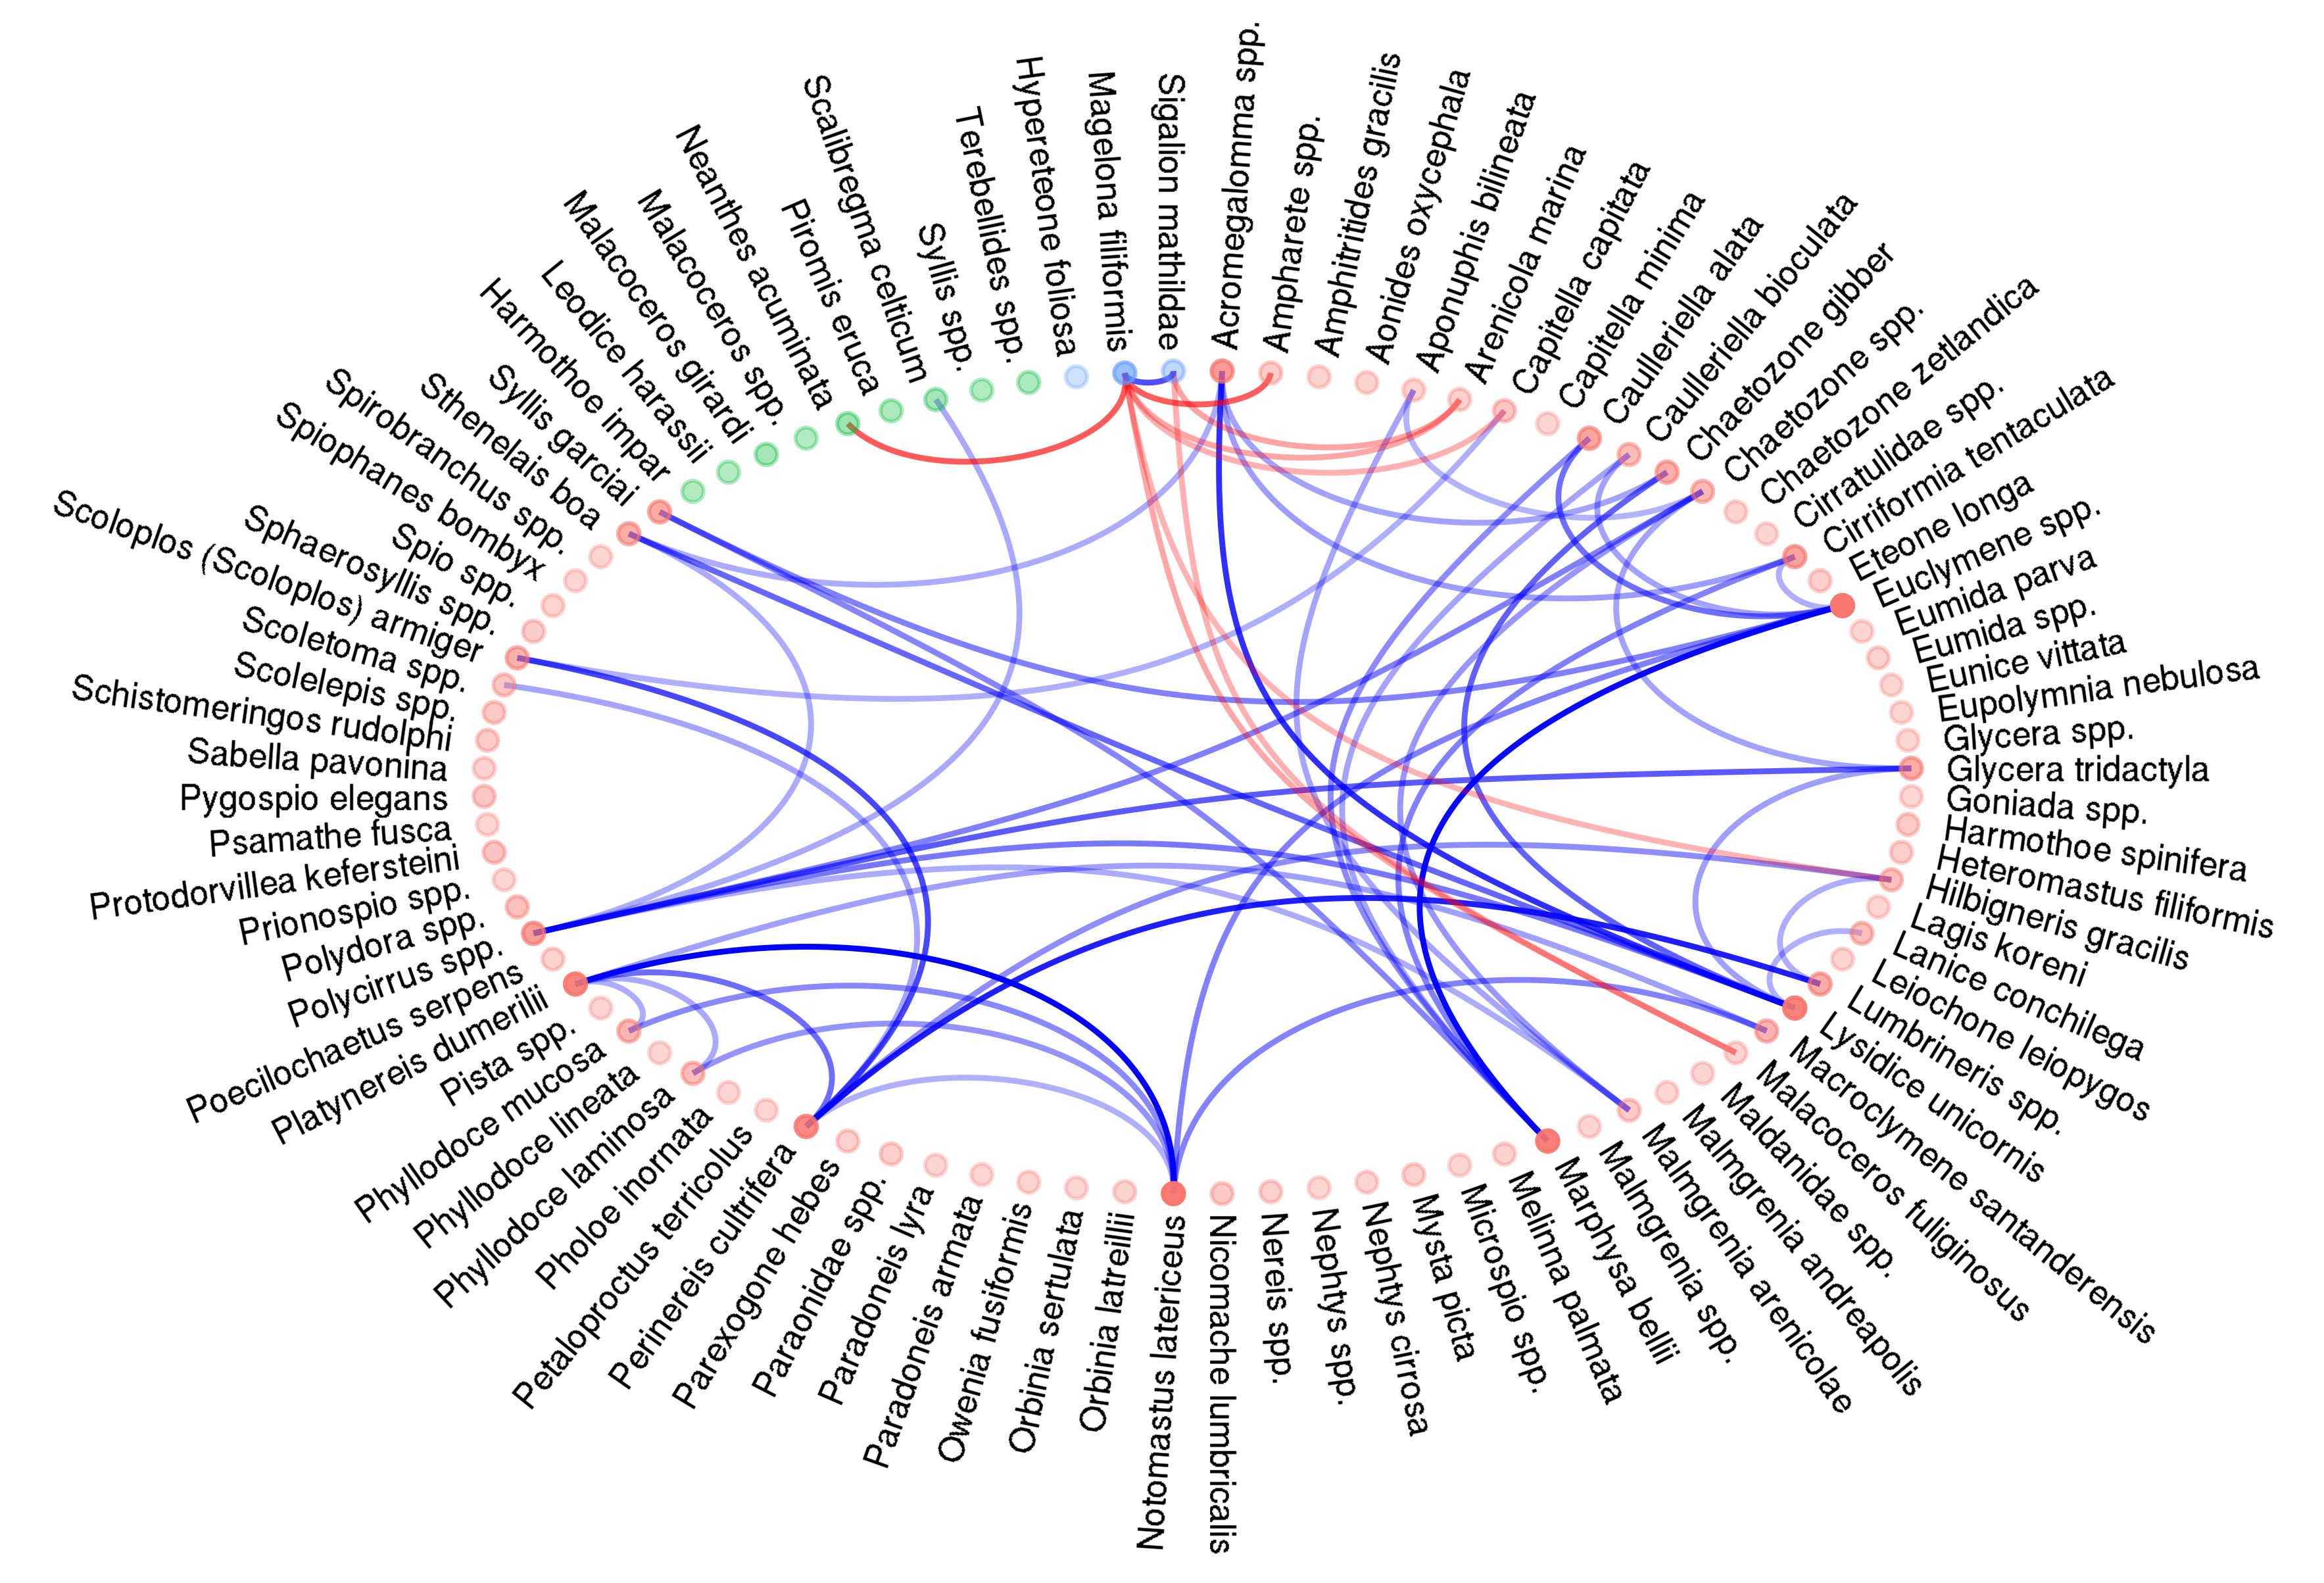
\includegraphics{figures/hmsc-hier-habitat-network-1.png}
\caption{Réseau reconstruit présentant les probabilités d'interaction
inférées par \emph{EMtree} sur la base des corrélations résiduelles
associées à l'effet aléatoire habitat du modèle \emph{HMSC\_hier}. Les
points rouges représentent les taxa de polychètes retrouvés dans les
deux habitats, les verts retrouvés uniquement dans les herbiers et les
bleus dans les sédiments meubles. Seules les arrêtes ayant une
probabilité supérieur à \(0,2\) sont affichées.L'opacité des arrêtes est
proportionnelle à leur probabilité. L'opacité des points est
proportionnelle à leur importance dans le
réseau.}\label{fig:nethmschierhab}
}
\end{figure}

\hypertarget{ruxe9sumuxe9}{%
\section{Résumé}\label{ruxe9sumuxe9}}

Prédire les facteurs qui biotiques et abiotiques qui contribuent à la
distribution des espèces au tour du monde est une tâche difficile. Ces
dernières années, une nouvelle catégorie de modèles de distribution
d'espèces est apparue : les modèles de distribution conjointe d'espèces.
En plus de variables climatiques, certains de ces modèles prennent en
compte d'autres types de données : comme des données phylogéniques ou de
traits fonctionnels. Ces modèles offrent deux perspectives : celle de
mieux prédire que les SDM classiques les patrons spatiotemporels de la
distribution espèces et de permettre d'accéder aux interactions entre
espèces. Observer et quantifier les interactions dans les écosystèmes
marins peut-être une tâche difficile, spécifiquement pour les
écosystèmes benthiques. L'utilisation de JSDM est un outil intéressant
pour pouvoir accéder à cette information. Ainsi, ce travail a eu pour
objectif d'explorer le potentiel de trois méthodes différentes de JSDM
sur un jeu de donnée d'abondance d'une communauté benthique pour
quantifier les effets abiotiques sur les patrons de diversité
spatiotemporelle et d'appréhender les interactions au niveau de la
communauté. Nos résultats montrent que tous les modèles expliquent
correctement une forte proportion d'espèces. Toutefois, les trois
modèles prédisent dans l'ensemble correctement la richesse spécifique,
néanmoins aucun d'entre eux n'est capable de prédire l'abondance. Nos
modèles montrent un fort effet des effets aléatoires, ce qui laisse à
penser que d'autres variables environnementales structurent ces
communautés biologiques. Enfin, les réseaux d'interactions reconstruits
grâce à ces méthodes ne font pas consensus chez un panel d'experts :
toutefois, certaines interactions sont correctement retrouvés par nos
modèles. Les JSDM sont donc des outils intéressants à utiliser en
écologie des communautés.

Predicting the biotic and abiotic factors that contribute to the
distribution of species around the world is a difficult task. In recent
years, a new category of species distribution patterns has emerged:
joint species distribution patterns. In addition to climate variables,
some of these models take into account other types of data: such as
phylogenetic data or functional trait data. These models offer two
perspectives: to better predict the spatiotemporal patterns of species
distribution than conventional MDS and to provide access to interactions
between species. Observing and quantifying interactions in marine
ecosystems can be a difficult task, specifically for benthic ecosystems.
The use of JSDM is an interesting tool to access this information. Thus,
the objective of this work was to explore the potential of three
different JSDM methods on a benthic community abundance dataset to
quantify abiotic effects on patterns of spatiotemporal diversity and to
understand interactions at the community level. Our results show that
all models correctly explain a high proportion of species. However, all
three models generally correctly predict species richness, yet none of
them is able to predict abundance. Our models show a strong effect of
random effects, suggesting that other environmental variables structure
these biological communities. Finally, the networks of interactions
reconstructed using these methods do not meet the consensus of a panel
of experts: however, some interactions are correctly found by our
models. JSDMs are therefore interesting tools to use in community
ecology. \%

%

\end{document}